\documentclass[10pt,letterpaper]{article}

\usepackage[margin=0.85in]{geometry}
\usepackage{fontspec}
\defaultfontfeatures{Ligatures=TeX}
\setmainfont{texgyrepagella-regular.otf}[
  BoldFont=texgyrepagella-bold.otf,
  ItalicFont=texgyrepagella-italic.otf,
  BoldItalicFont=texgyrepagella-bolditalic.otf]
\setsansfont{texgyreheros-regular.otf}[
  BoldFont=texgyreheros-bold.otf,
  ItalicFont=texgyreheros-italic.otf,
  BoldItalicFont=texgyreheros-bolditalic.otf]
\setmonofont{lmmono10-regular.otf}

\usepackage{amsmath,amssymb}
\usepackage{graphicx,float}
\usepackage{tabularx,longtable,booktabs,array,needspace}
\usepackage{cite}
\usepackage{xcolor,xurl}
\usepackage{pgfplots}
\pgfplotsset{compat=1.18}
\usepackage{microtype,parskip}
\usepackage[colorlinks=true,linkcolor=teal,citecolor=teal,urlcolor=teal]{hyperref}
\usepackage{bookmark}
\usepackage{fancyhdr}

\hypersetup{
  pdftitle={Slop Ninja: Writing transformation and AI detection on Bittensor},
  pdfauthor={Slop Ninja Research},
  pdfsubject={Subnet design whitepaper, draft 0.60}}
\setcounter{secnumdepth}{3}
\setlength{\emergencystretch}{3em}
\renewcommand{\arraystretch}{1.15}
\newcolumntype{L}{>{\raggedright\arraybackslash}X}
\newcommand{\tightlist}{\setlength{\itemsep}{0pt}\setlength{\parskip}{0pt}}

\pagestyle{fancy}
\fancyhf{}
\fancyhead[L]{\small\sffamily Slop Ninja}
\fancyhead[R]{\small\sffamily Design draft 0.60}
\fancyfoot[C]{\small\thepage}
\setlength{\headheight}{14pt}
\widowpenalty=10000
\clubpenalty=10000
\brokenpenalty=10000

\title{Slop Ninja\\[0.5em]
  \large Writing transformation and\\
  AI detection on Bittensor}
\author{Slop Ninja Research}
\date{November 2, 2026\\Draft 0.60}

\begin{document}
\special{pdf:minorversion 7}
\maketitle

\section*{Abstract}\label{abstract}

SlopNinja proposes an adversarial training subnet on Bittensor, pairing
mechanism \textit{A}'s AI detection with mechanism \textit{B}'s writing
transformation. \textit{B} is the main product objective: private models revise
authorized text toward the author's intended voice while preserving meaning,
readability, and tone. \textit{A} learns to detect AI involvement, including in
\textit{B}'s revisions; \textit{B} learns to remove unwanted formulaic prose and
evade \textit{A}'s detection. Public \textit{A} models supply training feedback
for \textit{B}, while authorized \textit{B} revisions provide challenging
examples for future \textit{A} training after evaluation retirement. This
competition is intended to improve both mechanisms; gains must hold on fresh
evaluation data. \textit{A} is also intended to supply author-fit feedback
against a private writer profile built from a user's own samples, which
\textit{B} would use alongside independent preservation and editorial checks
once a learned profile matcher qualifies. A lower detector score neither
establishes better writing nor changes a document's production history.

The subnet launches with \textit{A} alone as the initial evaluator and detection
service; \textit{B} activates after its editing, private-serving, and reward
requirements are qualified. \textit{A} is one text model with a shared encoder
for origin and attribution. It reports estimated AI-written or rewritten text
share and confidence in any AI involvement as separate percentages and
attributes human and model contributors. A span output locates AI-written
spans of at least 24 words, with per-sentence share and confidence; shorter
edits still count in both document percentages. AI-involvement Brier score is
the only reward quantity; share, attribution, and spans are qualification
gates. Every entry is to emit spans and, once the standing cohort template
enforces it, pass a span gate that compares its spans with SlopNinja's first
span package on the same batch, under margins fixed after measurement and
first run on live cohorts without enforcement. On a sealed,
pre-registered Test of passages whose human documents are excerpts of 150 to
450 words, the \textit{A} baseline's document model, the first reference,
was noninferior to Pangram
4.1, with balanced Brier 0.0518 against 0.0551 after both detectors' outputs
pass through maps fitted by the same method on a separate Calibration split, but the
pre-registered verdict failed because its three-seed recipe missed one domain
slice. SlopNinja's first span package leaves those document outputs
unchanged and adds a span head on a four-layer encoder tower, at about a fifth
more encoder time; since November 9, 2026 it is SlopNinja's span-serving
package. Retrospectively, on the consumed Test, it reaches character
F1 0.544 on spans of at least 24 words, finding 36\% of spans of 24--49 words
and 56\% of spans of 100 or more, and puts a span on 2.5\% of human
documents.
\textit{A} reads raw text and uses no context-free-grammar (CFG) features: a
CFG-only detector failed its first real-data test, and CFG writer vectors scored
below \textit{A}'s encoder on writer verification and added little on top of the
encoder plus stylometric features. Private writer profiles therefore use
\textit{A}'s encoder plus stylometric features; no profile tested so far is a
reliable author-fit signal.

\textit{B}'s proposed private adapters run in miner-owned Cloudflare accounts:
miners pay their model bills but must not receive customer prompts or responses.
Cloudflare and SlopNinja remain trusted operators; private weights must be
inaccessible to the general public. \textit{B}'s editing pipeline is planned
to use a shared English grammar for typed word, phrase, and clause edits and
for revision guidance. Mechanism \textit{C} credits accepted reusable
contributions to that grammar once. It activates by its own decision, which
may come before \textit{B}'s so the grammar can grow first, and is not required
for the \textit{A} launch.

One lead validator, operated by SlopNinja, serves as the coordinator.
The protocol below states requirements, and Section~\ref{implementation-status}
records which parts run today: the coordinator is specified to run entirely
serverlessly but remains unfinished, and testnet cohorts still run in a
separate evaluation service. Under the protocol, miners commit artifact digests
on chain and upload their model files straight to the coordinator's private R2
storage, which checks each file's declared SHA-256 on arrival. The coordinator publishes
the entrants' models, licensed CC BY-SA 4.0, when scoring starts, and scores
every entrant and the current and previous reference models (when a previous
one exists) on a fresh hidden batch of paired cases each day; SlopNinja publishes its own reference models on the same terms,
without evaluation text. Each batch is a fifth human-only, and on mainnet its human text comes
from Common Crawl pages captured before November 30, 2022, a historical-human
proxy drawn with capped domain shares that limit lookup by memorizing models and
checked by era gates; testnet uses a smaller public stock and, for cohorts
without a working outside entrant, reuses only documents already exposed;
every testnet cohort so far has drawn exposed documents only. The
protocol takes half of each batch's generated text from frontier models, to
which the coordinator has access through configured credentials, and half from
open models on Workers AI; Section~\ref{implementation-status} records
which of these steps testnet runs today.
Testnet starts from the first reference; mainnet later opens a fresh record of
cohorts with the reference testnet then holds. The reference changes when the
operator sets it by a recorded decision, as planned on testnet for the next
qualified reference, or when an entrant whose released score reaches the margin
cutoff also beats it by the margin in exact score and passes the promotion
checks. Rewards are paid on released scores: until a
cohort first has an entrant whose released score reaches the margin cutoff, or a
fallback cutoff once a previous reference exists, miner rewards burn, which under the documented emission rules also withholds the subnet's
TAO-side emission but not validator or owner alpha. Exact scores never leave the
coordinator: it releases only quantized scores, drawn with seeded noise under a
per-cohort privacy budget, shows each as soon as it is final, adds a few coarse
readings during scoring under a separate budget, and derives the canonical native weight row from them
with exact rules: subnet 78's geometric split of credit across score
bands and ranks, extended with a fallback cutoff for cohorts in which no gated
entrant's released score reaches the margin cutoff, no credit for detected copies of earlier
published models, a miner's own included, one credit shared among near-duplicate entries
and placed by the earliest-admitted entry's score, and
equal credit among equal quantized scores. The coordinator signs that row and publishes it
off chain; every other validator verifies and commits it, receives no held-out
data or exact score, and may check models or the row only in an advisory way.
The coordinator also signs, submits, and
recovers its own native weight commitments within the serverless service.
Validators commit the active signed row every tempo through native commit--reveal
in parallel, without waiting for the coordinator's own chain row, and keep
committing it through coordinator silence, since the authorization they commit
under never expires. A cohort lasts at least
20 tempos, about a day, ends with a transition that issues no new challenges,
and is paid during the following cohort. Slow work, missed wakeups, and
coordinator outages preserve the same cohort for recovery, and no record or
gate depends on a chain runtime version. No rule locks the operator out: it can
abandon a cohort, refuse to pay one, set the references, or switch to burn and
open a fresh record, each by a journaled decision with a signed public record,
the high-stakes ones under a separate offline key; none skips a cohort because
time passed or signs a commitment twice. A coordinator outage pauses the
protocol but not the chain or its emissions. Production applications use
Rust: native participants use \texttt{rtao}, while the coordinator is to run on
Cloudflare Workers with durable state and separately qualified chain integration,
woken by finalized-block notifications rather than a resident server.

Testnet runs for several months before the mainnet subnet is registered. On
November 7, 2026 its admission opened to every registered hotkey, and a
cohort with an outside entrant has since run end to end there. During this period
SlopNinja plans to earn revenue from free, advertising-supported public
detection pages served by \textit{A} and from other products. The revenue
accrues in a publicly visible pot that, once the mainnet subnet is registered,
buys and burns its alpha. The pot is to hold native TAO in a published
two-of-three multisignature account with an independent third signer, list
every payout, conversion, and burn publicly, and burn in daily tranches bound
to that registration; if SlopNinja abandons mainnet, the pot's TAO is
burned. The coordinator opens the paid detection service when measured
quality supports a bounded workload. Customers may fund quoted paid jobs by
card, TAO, or subnet alpha; their principal converts to alpha and is burned,
and does not directly reimburse serving costs. The detection page's paid API
settles through the pot instead. Burns are intended to support token value, with no guaranteed
market response. SlopNinja funds public-model execution and operating reserves
separately. Pricing and any emissions assigned to paid use require calibration
against measured costs, demand, and abuse incentives. The mainnet split of
emissions among owner, validators, and miners is not selected.

\clearpage
\section{Purpose and scope}\label{purpose-and-scope}

SlopNinja's primary goal is to transform writing so it sounds natural and
matches the author's intended voice. Mechanism \textit{B} serves that goal by
revising authorized text to remove unwanted formulaic prose and reduce detectable
model-writing patterns while preserving meaning, readability, and tone.
Mechanism \textit{A} supplies detection and attribution signals that support
\textit{B}'s revision search and evaluation, alongside separate preservation and
editorial checks. Together they form an adversarial training subnet:
\textit{B} trains against public \textit{A} detectors, and authorized
\textit{B} revisions challenge future \textit{A} training after evaluation
retirement. \textit{A} seeks to identify AI involvement even when \textit{B}
succeeds at reducing its visible signatures.
The subnet launches with \textit{A} alone; this development
sequence establishes a supporting evaluator and initial detection service
before the main writing product is qualified. Protocol sections state
requirements; Section~\ref{implementation-status} records which parts are
implemented today. A model, path, or component is \emph{qualified} once
recorded measurements or tests show that it meets its declared requirements;
qualification precedes activation.

\textit{A}'s origin detection estimates whether a document has human-only,
model-only, or mixed production history. Model-only and mixed work both count
as AI involvement under the declared labeling policy. The detector reports
confidence in any AI involvement and estimated AI-written or rewritten text
share as separate percentages, and attributes human and model contributors
where supported. It also locates AI-written spans of at least 24 words, with
per-sentence share and confidence (Section~\ref{span-outputs}); shorter edits
count toward both document percentages but are not localized. The scorer
serves span outputs, and once the standing cohort template enforces a span
gate, measured against SlopNinja's first span package on the same batch, every
entry must emit spans and pass it, while the reward stays document-level. Explanations
tied to particular words or constructions are later extensions.

Human writers have recurring habits of expression. Language models can also
exhibit characteristic choices in vocabulary, syntax, rhythm, and document
structure, shaped by training, tuning, and prompting. The proposed detector
learns these writing signatures through a shared origin-and-attribution model.
The hypothesis is that learning whose writing a text resembles helps determine
whether AI was involved. Signatures can overlap and change with prompts or
editing; they are statistical evidence, not unique identifiers. Their value
for AI detection must be measured on unseen writers, generators, and workflows.

\textit{A} learns these signatures from raw text and uses no grammar features.
A shared English grammar is planned as a later input for \textit{B}, where it
locates typed word, phrase, and clause edits and guides revision. Detector
evaluation can begin before transformation, private serving, or grammar
incentives are ready.

The three logical mechanisms have distinct jobs:
\begin{itemize}\tightlist
\item \textit{A}, AI detection and attribution: one text model estimates AI
involvement from production origin, matches human or AI-model profiles, and
locates AI spans of at least 24 words. Entrant models are
published, licensed CC BY-SA 4.0, when each daily evaluation cohort's scoring
starts.
Launch includes \textit{A} alone.
\item \textit{B}, authorized transformation: a private model proposes revisions
that improve fit to a writer's brief and reduce detector scores while preserving
meaning, readability, and intended tone. It activates separately.
\item \textit{C}, grammar improvement for \textit{B}: accepted reusable lexical
and structural contributions to the grammar that \textit{B} uses for edits earn
credit once, after a separate acceptance and reward protocol is qualified. It
activates by its own decision, possibly before \textit{B}.
\end{itemize}
These names describe workstreams, not three available native chain mechanisms.
The launch uses one native mechanism; later allocation must fit the chain's
supported mechanism interface (Section~\ref{benchmark-scoring-and-mechanism-mapping}).

\subsection{What a prediction means}

Origin is a production-history claim. Human-only, model-only, and mixed labels
refer to how a document was made under an explicit labeling policy. Attribution
instead asks which registered human or model profiles it resembles. A known
writer may use AI assistance; an unfamiliar model may produce text with no good
gallery match. Neither a matching human profile nor a low detector score proves
human-only origin. An unavailable prediction must remain an error or abstention,
never a default human label.

The launch evaluates English documents within declared length and resource
bounds. The evidence so far comes from passages whose human documents are
whole-paragraph excerpts of 150 to 450 words; other lengths need their own
measurements. Span outputs rely on retained exact span labels; multilingual
detection and manuscript-scale support each require suitable data and
measurements. Handling an embedded
foreign phrase, equation, or code block does not establish detection quality
for that language or content type. Predictions must retain uncertainty,
calibration context, and the limitations of the measured population.

We use \emph{slop} for defects in prose: vague or formulaic phrasing, needless
repetition, filler, and other patterns that weaken the piece. This is an
editorial definition, separate from production origin. Informal language,
unusual grammar, or a writer's recurring verbal habit may be appropriate to a
brief. The shared grammar planned for \textit{B}'s edits likewise describes
English as used, including errors and nonstandard forms, rather than enforcing
a prescriptive ideal.

\subsection{The grammar's role in later editing}\label{grammar-role}

A resolved parse exposes lexical choices, grammatical relations, and document
structure in a reusable representation. \textit{B} is planned to use the shared
English grammar to divide a source into typed word, phrase, and clause edit
units and to compare each revision with its source (Section~\ref{later-b}).
\textit{A} does not use it. The first real-data test of a CFG-only detector
failed, and adding CFG features to text gave only a small, uncertain gain, so
\textit{A}'s input contract is raw text (Section~\ref{input-contract}). A
head-to-head test of writer profiles found CFG writer vectors below
\textit{A}'s encoder on writer verification, by \(-0.034\) in AUC, simple
stylometric features above both, and only \(+0.0015\) from adding CFG to the
encoder plus stylometry, so private writer profiles use the encoder and
stylometric features (Section~\ref{writer-profile-evidence}). For \textit{B},
parsing costs money and time, and resolution can be wrong. Whether grammar-typed edits help
\textit{B}, whether \textit{C}'s contributions improve them, and any later
explanations each need their own evidence.

\subsection{Commercial thesis and users}\label{commercial-thesis}

The first paid product is hosted AI detection for applications, publishers,
researchers, and document workflows that need to assess AI involvement in
writing, with origin probabilities and attribution as additional detail.
\textit{A} artifacts become freely executable when their cohort's scoring starts. Paid
access, through the detection API or quoted jobs, offers maintained attribution profiles, bounded execution of a qualified
artifact, private delivery, and integration convenience. An \textit{A} detection job
runs the raw-text model alone, with no grammar parse. Publishing a model does not establish
that users will pay for hosting it; the commercial pilot must measure repeat
use, willingness to pay, false-positive disputes, and delivery cost.

Testnet runs for several months before the mainnet subnet is registered.
During that period SlopNinja plans to earn revenue from free,
advertising-supported public detection pages served by \textit{A} and from
other products, accruing in a publicly visible pot (Section~\ref{testnet-revenue}).
The pot pays the mainnet subnet's registration once it holds about 1.5 times
its cost. After the launch, the rest buys the subnet's alpha: half is burned,
and half is distributed to testnet miners in proportion to the revenue earned
by their winning models, those that beat the reference; all later revenue buys
and burns alpha.
The detection page itself carries no advertising and stores no text; ads run
on the site's content pages, and a paid detection API follows once the served package is
published. The pot is a published multisignature TAO account with a public
ledger of every payout, conversion, purchase, burn, and claim.
The coordinator decides when measured quality is sufficient to open sales and
which workloads may be sold. Benchmark eligibility alone does not enable
checkout. The initial price hypothesis aims below Pangram's standalone API
rate, subject to an independently evaluated quality comparison and measured
costs. The principal of a quoted paid job buys and burns alpha, while the
detection API's revenue joins the pot. Spendable operating
funds and refund reserves must come from an explicitly funded treasury,
independently of the burn (Section~\ref{revenue-and-costs}).

The main intended writing product, activated after the initial detection service,
serves users who supply samples of their own writing. A private writer profile
summarizes those samples from \textit{A}'s encoder and stylometric features;
\textit{A} compares successive revisions with that profile, and \textit{B} uses
its author-fit signal to guide editing toward the requested voice. No profile
tested so far ranks rewrites toward a writer reliably, so this workflow waits
for a learned matcher qualified on fresh writers
(Section~\ref{author-and-origin-detection}). It aims to
preserve every argument, qualification, attribution, and necessary detail while
improving voice and removing unwanted formulaic prose. Editorial quality and
production history remain separate: a revision of model-generated writing
retains that history even if readers prefer it or detectors miss it. Incremental
improvement and attainment of a strict detector target are also separate claims
(Section~\ref{transformation-and-improvement-utility}).

The intended adversarial training loop uses public detectors during
private revision search and reuses authorized revisions after evaluation
retirement. It must measure whether adaptive editing improves prose or merely
exploits the current judges. Writer consent and source rights limit training
reuse; customer jobs do not become benchmark material by default. The same
tools can be used to obscure provenance or impersonate a writer. Product claims
must preserve that risk and must not represent detector evasion as evidence of
human authorship.

\section{Participants and execution}\label{participants-and-the-two-kinds-of-work}

An \textit{A} miner trains a versioned text model for origin, share, span, and
attribution outputs. The artifact contains the weights, tokenizer, calibration,
and execution contract needed to run every output it declares. The miner commits only its
digest on chain and uploads the artifact privately to the coordinator, which
publishes it once the cohort ends. A published artifact, the miner's own
included, earns nothing when entered again, so a miner earns again only with a
model that differs measurably from every published one or improves on its
source by half the promotion margin (Section~\ref{public-copies}).
Slop Ninja executes
submitted artifacts for the pilot's hidden evaluations and published ones for
customer requests. Neither step requires the miner to operate a serving
endpoint or Cloudflare account.
Miners pay for their training and development; the operator pays for centrally
served \textit{A} inference. Benchmark rewards depend on measured performance,
not a claim about training expenditure.

Slop Ninja is the subnet \emph{operator}. The \emph{subnet owner} is the account
recognized on chain; Slop Ninja may operate through ownership or a lease.
A lease must secure an owner-authorized execution path for required
hyperparameter changes, including enabling commit--reveal, and any owner-only
burn operations. Operating the service alone grants neither those powers nor
the owner's emission entitlement.

One lead validator, operated by Slop Ninja, serves as the \emph{coordinator}.
This validator is the serverless service: it administers the daily frozen
evaluation cohorts, runs their models and the reference models, and
publishes a signed package of per-miner scores and the public inputs needed
to calculate rewards. It also calculates, signs, submits, and recovers its own
native weight commitments, then certifies its finalized row. These tasks all
run within the serverless deployment.
Every validator verifies the package and its receipt index, independently
applies the frozen reward rules, and derives the canonical
native weight rows. The same package and registration bindings must produce
identical integer UID/weight entries. Each validator uses its own key, nonce,
and recovery journal to commit and reveal those rows in parallel with the
others. No validator waits for the coordinator's reveal or finalized
row before committing. Held-out documents, labels, individual predictions, customer text,
and private model weights remain outside the public package. Other validators
do not reproduce the coordinator's hidden model scoring.
Section~\ref{cohorts} defines the package bindings, native submission rules,
and per-validator recovery requirements.

This pilot trusts the coordinator to execute and score honestly. Validator
recomputation checks reward arithmetic over the published scores; it cannot
establish that the reported predictions are real. After its own row finalizes,
the coordinator publishes a certificate for audit against the same
score package and derived row. Its certificate authenticates those bindings
without creating a validator quorum or a submission prerequisite.
The coordinator also decides when measured quality justifies offering paid
inference, and which workloads the service may accept. Commercial activation
does not revise a cohort's scores.

Dependence on other validators is confined to their timely native weight
delivery. Scoring, cohort advancement, and customer service require no validator
quorum and do not depend on other validators' acknowledgments, availability,
software updates, or migration completion. Each validator submits and recovers
independently; delayed validator rows affect native reward allocation
without holding evaluation or service work open. The coordinator's own chain
delivery and certificate publication also do not gate cohorts or other validators.

Curators maintain authorized evaluation collections, production histories,
hidden labels, and source-group splits. Access to these materials follows the
collection's permissions. Customers authorize processing of submitted documents
and reference writing under their declared rights for a quoted job; buying inference gives no automatic
permission to add either to training or benchmarks. Author references and
derived profiles receive the same content protection as the query document.

Later \textit{C} contributors submit public grammar and lexical improvements.
Accepted contributions receive credit once under a separately activated
contribution contract (Section~\ref{grammar-contributions}). Later \textit{B}
miners register private transformation pipelines, with language-model adapters
served by Cloudflare in their own accounts and numeric rankers executed by
Slop Ninja. These miners maintain their delegated access, capacity, and billing,
and pay for their model calls, including required evaluations. Customer
payments follow the burn policy; no direct per-job reimbursement is promised.
Neither \textit{B} service obligations nor \textit{C} rewards apply to the
\textit{A}-only launch.

\subsection{Rust applications and serverless execution}

All Slop Ninja production application logic is written in Rust, including
native miner and non-coordinator validator clients, update and migration tools,
and the serverless coordinator, challenge, and inference logic. A \emph{challenge}
is a coordinator-internal evaluation task, such as generating cohort documents
or running an admitted artifact on them; no challenge is sent to a miner or
validator. Native participants use
\texttt{rtao} for chain integration~\cite{rtao}; Linux and macOS releases require
explicit platform qualification. Research ML backends remain separate from
this production contract. Native participants retain their own hotkeys.
The coordinator's validator hotkey is controlled within the serverless service,
with durable signing ownership and transaction recovery. Its authorization and
receipt keys remain distinct from that hotkey; other validators' keys never
enter the service.

Miner and validator clients install signed updates automatically and
independently. A participant that has missed several releases follows the
supported sequence of resumable schema migrations before resuming its work.
Updates preserve unfinished obligations and reconcile chain submissions before
retrying them. No participant waits for another to update or migrate. The
release, migration, and conditional rollback requirements appear in
Section~\ref{cohorts}; automatic recovery must satisfy its compatibility and
journal checks before new signing is allowed.

The coordinator is entirely serverless on Cloudflare Workers and Durable
Objects~\cite{cfworkers,cfdo}. Shared Rust code defines canonical messages,
artifact identities, scoring, and state transitions; supported modules compile
to Wasm with the required platform bindings and generated deployment glue.
The full native \texttt{rtao} runtime is not assumed to compile into a Worker.
Workers code follows a bounded-memory rule: it allocates only inside a fixed
arena sized from measured peaks, checks every declared length against that
budget before allocating, and streams large objects instead of buffering or
re-reading them.
The coordinator needs qualified Workers-compatible chain transport, encoding,
signing, and durable reconciliation, including its validator commitments and
reveal obligations. Both coordinator and native participants use the
\texttt{rtao-rpc} service, which provides Slop Ninja RPC
access at no service charge~\cite{rtaorpc}. Chain fees and execution costs remain
separately funded.

Live \texttt{rtao-rpc} webhooks, offered for both Finney and testnet, deliver
every finalized block. That per-block delivery is the coordinator's primary
heartbeat and clock, and each delivery is its own Worker invocation~\cite{cffetch}.
Durable Objects retain the finalized block cursor, and RPC reads backfill gaps
and resolve finality. A one-minute Cron Trigger~\cite{cfcron} is the only
fallback: when deliveries stall, including after the provider pauses a
subscription whose retries are exhausted, it processes blocks from public
OpenTensor RPC through the same per-block path. No permanently running
subscriber is required. A webhook is a notification, not evidence of finality or
permission to sign. Section~\ref{block-notifications} specifies ingress, the
cursor, fallback, and the operator-resumed pause, a stated limit; the webhook
receiver and the serverless chain path remain integration work.

\begin{table}[H]
\centering
\begin{tabularx}{\linewidth}{@{}lX@{}}
\toprule
Component & Responsibility \\
\midrule
API Workers & Enrollment, authenticated requests and block-webhook ingress,
status, and result retrieval. \\
Durable Objects & Authoritative cohort checkpoints, admission, reservations,
accounting, finalized-block cursors, and the coordinator's chain journal and
signing ownership. Each record has one transactional owner. \\
Lane Durable Objects & Execute fan-out lanes of bulk evaluation work. Each lane
claims tasks under the cohort object's durable leases, runs in its own
invocation, drives its own Container instance for model runs, and persists
outcomes before releasing its claim. \\
Queues & Carry lane wakeups holding identifiers and generations only; durable
lane records reconstruct any lost, duplicated, or expired message. \\
R2 storage & Versioned artifacts, evidence, manifests, and encrypted private
job objects, bound to their durable records by identity and digest. \\
Cron watchdog & Detect stalled deliveries or cursor lag, then process
finalized blocks from public RPC through the per-block path until webhooks
resume. \\
\bottomrule
\end{tabularx}
\caption{The serverless coordinator. Queue delivery, lane invocations, and
wakeups do not own protocol state.}
\end{table}

Task identities and dispatch intent are persisted before queue delivery, and a
lane's assignment is recorded in the cohort object before its wakeup is sent.
Messages carry identifiers and checkpoint generations, never customer content
or credentials. A lane checks the current authorization and claims the
recorded task before acting. Duplicate delivery cannot create a second
accounting outcome. External execution can still repeat after an uncertain
timeout; bounded retries retain every attempt and apply a declared selection
rule. Queue retention is finite, so durable records must reconstruct pending
dispatches after a long pause~\cite{cfqueues}. Cross-object work uses persisted
idempotent messages; a transaction in one Durable Object cannot atomically
update another~\cite{cfdo}.

All production inference, challenge generation and execution, and scoring run
serverlessly. Parsing and model execution take place outside the objects that
serialize admission and accounting. Bounded Rust/Wasm computation runs in
Workers; a qualified Cloudflare serverless Container under Slop Ninja's control
supplies bounded computation beyond their limits, including every \textit{A}
model run. Workers AI supplies supported language-model and adapter formats; it
cannot host the \textit{A} encoder
(Section~\ref{existing-evidence-and-implementation-status}). Bulk evaluation
work runs as fan-out jobs: the cohort's Durable Object divides challenge
generation, paired scoring, receipt bundling, and per-model score summaries
into lanes, at least one per scored artifact and more as the batch grows
(Section~\ref{fan-out}). Each scoring lane drives its own Container instance,
and generation lanes share one rate limiter. Lane count changes elapsed time and
per-lane start cost, never a document's outcome. Every workload needs measured CPU, memory, bundle,
and numerical-runtime limits before admission; these targets do not imply
support for arbitrary uploaded architectures. Miner-supplied executable plugins
are excluded. Coordinator state and scheduling remain in Workers and Durable
Objects, and production serving never depends on a miner's or validator's local
machine being online.

The native adapter uses durable \texttt{rtao} journal and weight/reveal recovery
APIs. It starts paused, reconciles finalized history, and requires explicit
resumption with application compatibility checks. This is an integration
component, not a deployed validator. Its tested scope and current limitations
are recorded in the ``Implementation boundary'' paragraph in
Section~\ref{native-implementation-boundary}; unsupported paths
require completion and qualification before deployment. The coordinator's
Durable Object journal must implement the same intent, attempt, and finalized
recovery requirements as the native validators' local journals; the native
file-backed implementation does not supply that storage adapter. The cohort
recovery contract in Section~\ref{cohorts} applies to both deployments, including
the evidence needed to resume after runtime upgrades or missed tempo boundaries.

\section{Model interfaces and qualification}\label{model-interfaces-and-starter-architectures}

Launch admits one \textit{A} model per entry. The model predicts AI share,
production history, author identity, and AI spans in one invocation. All output heads
must consume a common document encoding produced by a shared learned encoder;
each may also have task-specific layers. This requirement enforces one shared
encoding interface; whether the heads use common predictive features requires
measurement. Admission checks this structure in the
submitted computation graph, together with one manifest and input/output
contract. Packaging two independent predictors behind one API does not qualify.
This checks inference structure, not whether the components were trained jointly.
Known AI models have predefined author profiles alongside human
writers. Detecting AI involvement is the primary purpose of the origin output
and the only reward quantity; the other outputs are qualification gates. The
transformation mechanism \textit{B} is deferred to Section~\ref{later-b};
\textit{C}'s proposed contributions to the shared grammar that \textit{B} uses
appear in Section~\ref{grammar-contributions}.

The shared encoder is intended to let the two tasks improve each other.
Learning author- and generator-specific writing patterns can help identify
model involvement. Production-history supervision can help attribution
distinguish a writer's habits from patterns introduced by generation or
editing. Both objectives can therefore shape features useful to the other.
This expected mutual benefit requires measurement: sharing an encoder alone
does not establish it. Section~\ref{development-and-launch-criteria} requires
each new architecture to be tested in both directions against models trained
for each task alone.
The requirement deliberately gives detection, attribution, and later author-fit
feedback one reusable learned representation. Graph inspection cannot establish
useful feature sharing; disjoint slices could satisfy the structural rule.
Measured harm would prompt an explicit revision of the design before launch,
rather than an undocumented exception to admission.

An \textit{A} entrant submits the weights and all data needed for the declared
inference calculation. The artifact stays private until its cohort's scoring
starts and is published then (Section~\ref{a-artifact-execution}). Miner
submissions are licensed CC BY-SA 4.0, so anyone may obtain a published artifact
free of charge and execute it locally, and later \textit{B} development is
expected to train against published detectors. A published artifact stays
public and is never recalled. The coordinator deletes its private admission
copy once the cohort closes and publication is recorded, and keeps the current
and previous reference artifacts hosted for evaluation while they are
references (Section~\ref{cohort-receipt-retention}). Hosted execution through
the paid API is charged separately.
Miners may keep their training recipes and permitted training corpora private.

Project code and documentation are licensed MIT OR Apache-2.0, except files and
datasets that carry their own licence or notice. Reference weights are licensed
CC BY-SA 4.0, like miner submissions, and Slop Ninja publishes its own
references, \(R_0\) and any later reference it trains
(Section~\ref{reference-model}), on the same terms. A public reference package
carries no evaluation text: its replay cases are synthetic rather than
development documents, and the package passes a scan for corpus text before
release. \(R_0\) is published once its package has been re-exported in this
way. Miners can also start from a public training recipe~\cite{trainingguide}:
it fine-tunes ModernBERT-base on about 4,200 Train rows from five
redistributable dataset snapshots and packs and checks an admissible artifact
with the miner client. It reproduces \(R_0\)'s pipeline and artifact format,
not its V6 starting point, data, or weights, and is not a strong detector. An
entrant artifact that becomes the reference was already published with its
cohort.
Slop Ninja executes submitted artifacts for the pilot benchmark and published,
qualified artifacts for customer service; an \textit{A} miner needs no private
serving account or delegated inference credential.

\subsection{AI detection through origin and attribution}\label{author-and-origin-detection}

The origin output is a calibrated probability distribution over three recorded
production histories: human-only (\(p_{\mathrm{human}}\)), model-only
(\(p_{\mathrm{model}}\)), and mixed human/model work (\(p_{\mathrm{mixed}}\)). The
artifact combines model-only and mixed probabilities to answer the primary
AI-involvement question. It reports a continuous probability, displayed as a
percentage:
\[
 p_{\mathrm{AI}} = p_{\mathrm{model}} + p_{\mathrm{mixed}},
 \qquad
 \texttt{ai\_confidence\_percent} = 100\,p_{\mathrm{AI}}.
\]
Binary training labels are zero for documented human-only work and one for
model-only or mixed work. The model learns a probability from those labels;
it does not convert a hard decision into a percentage. Documented three-way
histories additionally supervise the origin components. The three probabilities
sum to one, and their calibration method and workload profile are frozen with
the artifact. Every completed inference returns numeric share and confidence
scores. An unavailable prediction returns an explicit failure status, never
zero scores. Fixed
thresholds remain useful for benchmark operating points but are not required
public outputs.

The second percentage is estimated AI share: the expected fraction of final
words in model-written or model-rewritten spans under the provenance convention
in Section~\ref{training-data-and-evaluation-separation}. Write that fraction
as \(f_{\mathrm{AI}}\) and its predicted expectation as \(\hat f_{\mathrm{AI}}\):
\[
 \texttt{ai\_share\_percent}=100\,\hat f_{\mathrm{AI}},
 \qquad 0\leq p_{\mathrm{model}}\leq\hat f_{\mathrm{AI}}\leq p_{\mathrm{AI}}\leq1.
\]
These bounds follow because human-only work has zero share and model-only
work has unit share under this convention. One implementation uses
\(\hat f_{\mathrm{AI}}=p_{\mathrm{model}}+p_{\mathrm{mixed}}\mu_{\mathrm{mixed}}\),
where \(\mu_{\mathrm{mixed}}\in[0,1]\) is the learned expected share conditional
on mixed history and the document. Binary labels supervise confidence; measured
fractional labels additionally supervise share. A result can therefore report
20\% estimated share with 99\% confidence that AI contributed. Confidence is
the probability of involvement, not certainty that the share estimate is exact;
uncertainty intervals for share require separate validation. Both percentages
must qualify on their declared workloads before paid service.

Attribution reports conditional results for both human and AI-model roles.
Each result names supported gallery matches, or returns \emph{Other human}
(\texttt{other\_human}) or \emph{Other AI} (\texttt{other\_ai}) when no named
profile for that role satisfies the frozen matching rule. The question is
which contributor fits \emph{if that role contributed}; a conditional match or
fallback does not itself assert that the role is present. Report its involvement
probability alongside it:
\[
 p_{\mathrm{human\ involved}}=p_{\mathrm{human}}+p_{\mathrm{mixed}},
 \qquad p_{\mathrm{AI\ involved}}=p_{\mathrm{AI}}.
\]
These probabilities may sum above one because mixed work includes both roles;
they are not shares of the text. No presence cutoff suppresses a role's
attribution. Both fallbacks can therefore appear for mixed work, including
when neither contributor has a named match. Multiple contributors need not
be forced into one identity.

The fallback categories are outcomes, not enrolled profiles or assertions
that an identity is absent from the gallery. A listed writer or model may be
unidentifiable from the available text. There is no separate unknown or
attribution-abstention label in a completed result; failure remains separate.
Supported named-model matches remain visible even at low AI-involvement
probability, without changing that probability or proving authorship.
The output contract fixes these meanings and their calibration before evaluation.

Origin and attribution answer related but different questions. An unseen generator
may receive high AI confidence and \emph{Other AI} attribution. Failure to match a
known model does not establish human origin. A known writer's style may survive
AI assistance, so a human-profile match cannot override the origin estimate.
When a model rewrites human-only text, the resulting work has mixed history.
When one model rewrites another model's draft, it remains model-only under the
initial label policy, with attribution potentially unresolved. The outputs
estimate the recorded workflow and its contributors; they do not prove authorship.

Independent reference works form the gallery. Its construction, pooling,
reference/query roles, and version are part of the inference contract. The
interface should permit enrollment of a new human author from independent
samples without fitting another permanent identity classifier. Profile IDs
identify output matches and gallery entries; they are excluded from query
features.

The main intended human-attribution workflow is personal: a customer supplies
their own writing samples to construct a private writer profile. A qualifying
match returns \emph{Provided writer} (\texttt{provided\_writer}), bound to that
customer's selected reference profile. This is a named match under the normal
matching rule; if no human profile qualifies, return \emph{Other human}. It can accompany
AI involvement and identifies resemblance to the supplied writing, without
authenticating the customer's identity or proving authorship. The profile is
scoped to the request or customer account and is never implicitly enrolled in
the public gallery. Operator-maintained human profiles may also use documented
public or licensed references under a published enrollment policy recording
provenance, the identity basis, and permitted uses. Public availability alone
does not settle those uses.

In this later workflow, trusted preprocessing represents each reference work by
\textit{A}'s encoder output and by stylometric features, function-word
frequencies and character n-grams, then pools them into one writer profile under
a qualified, versioned pooling contract. A normalized weighted mean is the
initial candidate; the contract fixes feature scaling, per-work weights,
missing-channel handling, and the compatible encoder, feature, and pooling
versions. The
matcher receives the profile instead of raw reference prose. A pooled summary
need not represent any single work, so qualification must test whether
averaging loses useful variation across topics or registers and whether sample
length or an outlier dominates the result. Raw samples are still read during
trusted preprocessing. Both samples and profiles receive customer-content
protection; a profile is not an anonymization method. The same fixed profile is
the intended target for later \textit{B} revision using \textit{A}'s continuous
author-fit feedback (Section~\ref{author-transformation-and-detector-evasion}).

No profile type yet qualifies to back \emph{Provided writer} or that feedback.
In an October 31, 2026 comparison on writers neither system had seen, unlearned
profiles from \(R_0\)'s encoder beat CFG writer vectors on verification,
stylometric features beat both, and adding CFG to the encoder plus stylometry
gained only \(+0.0015\) in AUC, so CFG writer vectors are not a profile
channel. Encoder plus stylometry was the strongest
profile, yet at five references 42\% of impostor trials still passed when 90\%
of genuine ones did, and no profile ranked rewrites toward a target writer much
above chance (Section~\ref{writer-profile-evidence}). The next qualification is
a learned matcher trained on fresh authors, with its acceptance thresholds
measured on withheld writers and on real style-transfer data. Until a profile
type passes it, neither \emph{Provided writer} nor \textit{B}'s author-fit
feedback is offered.

Open-set rejection is evaluated on withheld writers and
generators, separately from choosing among known profiles. Rejection means a
completed attribution decision that accepts no named match for the evaluated
writer or generator role, including \emph{Other human} and \emph{Other AI}.
Evaluate each documented contributor role, including both roles in mixed work,
regardless of its predicted probability. Credit successful rejection only when
the ground-truth identity is absent from the gallery and the corresponding
fallback accepts no named match for that role. A wrong named match is an
attribution error; fallback on a listed identity is not successful open-set
rejection. Missing role results and execution failures remain in the assigned
population and earn no rejection credit. Do not score conditional identities
for roles absent from the documented history; evaluate mistaken involvement
probabilities through origin calibration and false-positive measurements.
This role-level rejection rule covers one contributor or a role whose
contributors are all withheld. A role containing both known and withheld
contributors needs a frozen set-valued attribution metric before earning
rejection credit; retain such cases in coverage and report them separately.
Launch qualification covers English documents. Multilingual claims and
additional document-length classes need their own data and workload evidence.

\subsection{AI span localization}\label{span-outputs}

The goal is to locate AI-written text, not only to score whole documents.
Sentences are one view of that location. The output contract therefore adds a
token-level head on the shared encoder. It returns an AI probability for every
token, decodes those probabilities into AI spans with exact character offsets
into the canonical text and a confidence for each span, and derives per-sentence
AI share and AI-involvement confidence from the same token probabilities. The
document-level outputs keep their meanings, and the span outputs are made to
agree with them by construction. In the runtime's emission, a word's
probability is the mean probability of its tokens, and a share tilt shifts every
word's logit by one common bias so that the mean word probability equals the
emitted document share. A sentence's
share is the mean tilted probability of its words, so sentence shares aggregate
to the document share by final-word counts over complete, nonoverlapping
partitions. Document involvement confidence cannot be assembled that way,
because neighboring sentences are dependent: neither averaging sentence
confidences nor multiplying their complements yields a document probability.
It remains the document head's calibrated output, and sentence and span
confidences are capped at it.

The training labels already exist: retained exact model-produced spans for mixed
documents, all-AI labels for model-only documents, and all-human labels for
human-only documents (Section~\ref{training-data-and-evaluation-separation}).
Qualification measures token-level Brier score, character-span intersection over
union and F1 against the retained spans, span-boundary error, and sentence-level
calibration. Each cohort reports these measures as a qualification gate whose
thresholds are fixed after measurement; span outputs earn no reward, and
document involvement Brier remains the reward. Agreement with the document
outputs needs no gate, because the emission guarantees it; the gap between mean
word probability and document share before the tilt is reported as a
diagnostic, since the tilt costs word-level accuracy wherever the document
share is the less accurate estimate. The span gate includes the
false-positive rate of human sentences inside mixed documents, reported
separately from the pure-human document gate, because identical human words
score higher next to AI text than alone (Section~\ref{cohort-mix-evidence});
like every span measure it carries no reward weight.

The release package pairs \(R_0\), the first reference model, with such a head
(Section~\ref{span-evidence}). The head was
trained on \(R_0\) with the encoder and document heads frozen, so its document
outputs are bit-identical to \(R_0\)'s. Its decoder was chosen under a limit of
spans on at most 22 of 570 development human documents, which it meets with no
slack. On held-out spliced rewrites it reaches mean per-document character F1
0.410 and recall 0.402, counting a document without a decoded span as zero, and
precision 0.862 over the documents in which it decodes one.
It decodes no span in 42\% of those documents and mostly misses clause and
single-sentence edits, at character F1 0.051 and 0.167. Retrospectively, on the
consumed sealed Test, 2.5\% of human documents carry a decoded span, and text
written by a base model is almost never found. A joint fine-tune of encoder and
heads found more spans but scored human documents clearly worse before
calibration, so it was not adopted.

Slop Ninja has adopted a follow-up head, S2c, as its span head for the first
package that serves spans; until span serving lands, the shipped head above
stays in the release package. S2c keeps the encoder and document heads frozen
and feeds the token head through a trained copy of the encoder's last four
layers and final norm. Its document outputs are byte-identical to \(R_0\)'s at
every seed, so confidence, share, and reward scoring do not change. Its own
decoder puts spans on 21 of the 570 development human documents, within the
limit, though seeds 29 and 41 give 22 and 27. Compared without span calibration
maps, on the held-out spliced rewrites it reaches character F1 0.519 and span
F1 0.485, against 0.410 and 0.241 for the shipped head (0.245 with its maps);
retrospectively, on the consumed Test, its mixed-document character F1 is 0.535
against 0.478, but with calibration 3.4\% of human documents carry a span
against 2.5\% (Section~\ref{s2c-evidence}). The tower adds 18--20\% of the
encoder's CPU time and about 20 million parameters, which puts such a graph
outside both allow-listed graphs and above the 160 million parameter limit
(Section~\ref{a-artifact-execution}); admitting such a graph needs a versioned
manifest that widens both. No calibrated package with S2c has been built or
replayed yet. \(R_0\) remains testnet's first reference, and no span package
is named \(R_0\) (Section~\ref{reference-model}).

Until a cohort manifest enforces the span gate, the token-level head is
optional and its outputs are reported without affecting eligibility; from that
manifest on, every entrant must provide it. The allow-list names the graph with
the token-level head from launch, but the scorer does not run span heads yet,
so admission refuses that graph until span serving qualifies
(Section~\ref{a-artifact-execution}). Enforcing the gate does not by itself
change the reference; reference changes follow Section~\ref{reference-model}.

A further extension could identify words and constructions that materially
influence a score, starting from the token-level outputs. Test explanations by
removing or changing the cited text and measuring the model's response with
meaning and context controls. Require stability across innocuous formatting
changes. Explanations in terms of grammatical constructions belong to later
\textit{B} revision guidance, which uses the shared grammar. An
influence on a model score is evidence about its calculation, not proof that a
word or construction was produced by AI. Attention weights or a generated
explanation alone do not establish that influence. These explanations are a
separate future qualification, not an initial launch requirement.

\subsection{\textit{A} input contract: raw text}\label{input-contract}

The \textit{A} input is the canonical document text. A miner artifact is a
text model: an ONNX computation graph, a fixed tokenizer, the output heads, and
their calibration. The coordinator tokenizes each document with the
allow-listed tokenizer, which the artifact's own must match byte for byte, and
runs the graph on CPU in a Slop Ninja-controlled Cloudflare
Container under the cohort's declared length and resource limits; an input beyond the artifact's limit returns an explicit
unsupported-length result. Cohort batches stay within the declared profile.
While the span gate is inactive, an entrant with document heads only, like
\(R_0\), is admissible (Section~\ref{span-outputs}).
The reference \(R_0\) is a ModernBERT-base encoder~\cite{modernbert} of
about 150M parameters with a 2,048-token limit, fine-tuned from the earlier V6
detector on raw tokens, with origin, share, and attribution heads
(Section~\ref{existing-evidence-and-implementation-status}); the release
package adds the token-level span head. Its architecture,
with or without a token-level span head, defines the graphs that admission
allows (Section~\ref{a-artifact-execution}).

\textit{A} uses no features derived from a resolved context-free-grammar (CFG)
parse. A CFG-only detector failed its first real-data test: on an October 26,
2026 research Test of 102 documents
(splits as in Section~\ref{splits}),
CFG-only shared models had AI-involvement Brier 0.126--0.134 against 0.096 for a
Calibration-mapped Pangram comparator on the same documents, and flagged
67--87\% of human documents at the 0.5
cutoff~\cite{cfgviability}. Adding CFG coordinates to frozen text features gave
only a small, uncertain Development gain, 0.048--0.057 against 0.052--0.058 for
text alone~\cite{v6cfgfusion}. Those tests used pooled grammatical-leaf counts;
ordered and tree-aware CFG inputs remain untested. Parsing and ambiguity
resolution also add latency and cost, and numeric features carry information
about the source, so they provide no confidentiality guarantee.

The grammar's planned uses are \textit{B}'s edit representation, which types
edits and places a revision alongside its source (Section~\ref{later-b}), and
\textit{C}'s contributions to it (Section~\ref{grammar-contributions}); neither
depends on \textit{A}'s input contract. Any change to that contract, including
grammar features, would need a new paired comparison against raw-text models,
including its added cost, before admission
(Section~\ref{development-and-launch-criteria}).

\subsection{Artifact submission and execution policy}\label{a-artifact-execution}

An execution manifest fixes the whole calculation: weights, input/output
schema, feature meanings and order, normalization, availability masks,
serialization, calibration, reference pooling, numerical precision, rounding
and tolerances, admitted operators, dependencies, resource bounds, and
reference outputs. It also fixes the tokenizer and the canonical text profile.
Names, handles, and other identity-bearing material follow the profile's
declared policy. Explicit author IDs, miner UIDs,
assignment metadata, hidden labels, and source/candidate-role flags are
excluded from learned query inputs.

Models within a comparison receive the same accepted text. A change to the
input profile begins a new comparison and requires requalification;
it cannot silently alter an unfinished cohort. Weight, calibration, or other
inference-semantic changes create a new artifact version. Compatible
operational repairs may preserve those semantics under the cohort rules in
Section~\ref{cohorts}. In particular, replacing an execution host must preserve
the artifact and calculation rather than substitute a different detector.

The coordinator caches the cohort batch, executes qualified artifacts under
equal limits, and retains their predictions and failures. Centrally executing
submitted artifacts keeps hidden benchmark inputs out of miner request paths
and limits direct benchmark harvesting. Model isolation and operator access
controls remain necessary. Publishing each executable when its cohort's scoring
starts permits inspection and independent experiments.
Validator duties follow Section~\ref{participants-and-the-two-kinds-of-work};
the scoring trust assumption is stated in
Section~\ref{trust-assumptions-and-adversarial-behavior}.

The manifest's allow-list names two graphs: the reference's ModernBERT-base
architecture and the same architecture with the token-level span head, each
with matching operators and shapes and integer arithmetic on token identifiers
only in the embedding lookup. An artifact has at most 160 million
parameters; \(R_0\) has 149.6 million. Its tokenizer must match the
allow-listed tokenizer byte for byte. Its calibration, contract, and other
declared files must validate against fixed schemas for their roles, such as a
monotone piecewise-linear calibration map whose knot count the schema bounds,
and a file without a declared role is rejected. These rules bound the total
size at about 700 MB, against the 610.6 MB of \(R_0\)'s artifact object, whose
graph file is 601 MB, so no separate byte cap
applies. The scorer serves only the graph without the span head today, so
admission refuses the span graph, recognized from the graph file's length in
the artifact object's header (below), until span serving
qualifies~\cite{artifactspec}. Where a limit is needed it derives in this way from structure, such as
the allow-list, a schema, or a measured bound, and is versioned in the manifest
rather than hard-wired, because a fixed limit that later models outgrow can
strand a subnet. The allow-list widens only through a versioned manifest. The
cap bounds what an artifact can memorize, an estimated 40--72 MB of learned
capacity, and an embedded index or lookup table
of text fails admission (Section~\ref{lookup-exposure}). The scorer has no
network access, online learning, cross-job prompt cache, or undeclared mutable
state. Qualification exercises resource bounds and numerical
boundary cases on the actual admitted runtime. Linux and macOS tooling may
inspect and prepare artifacts, but outputs from another backend become
interchangeable only after numerical qualification.

Qualification uses independently labelled hidden material and includes
formatting variants, identity and topic leakage, targeted triggers, chosen-input
failures, exact or near-copy submissions, and batch invariance: each document's
outputs must be identical whether it is scored alone or among its batch. Canonicalization does not replace
these controls. A publicly reproducible calculation can still exploit a
benchmark shortcut or favor a collaborator. These checks inform qualification
and continuing evaluation without establishing universal robustness.

\paragraph{Artifact objects.}
An artifact object is a length-prefixed header of at most 1 MiB, listing each
file's path, role, SHA-256, and length, followed by the files in path order.
The graph, weights, tokenizer, calibration, and output-schema files form its
inference content; reference test vectors, owner metadata, and publisher
signatures do not. The inference-content digest covers the frozen contract and
each inference file's role, digest, and length, so renaming or re-signing an
artifact cannot create new inference content. Two inference files with the same
role, digest, and length are refused. The object is the miner's local file and
its published form, but it is uploaded and published as the header and each
distinct file separately, from which anyone can rebuild it. The miner hashes
each file when it packs the artifact, and R2 computes each object's SHA-256 as it
arrives to check the declared digest; no Slop Ninja code hashes a model byte
after packing: the graph's class is checked by comparing its structure, the graph
file without its weight values, byte for byte with the allow-listed class's
pinned reference bytes~\cite{artifactspec}.

\paragraph{Private submission and duplicate credit.}
A miner commits on chain only a digest. Through the chain's commitment call, it
publishes a domain-separated commitment binding the chain and subnet, the
cohort, its hotkey and registration generation, the inference-content digest,
and a fresh secret 256-bit nonce. The commitment binds the inference content,
not the object's bytes, so objects that differ only in excluded files open the
same commitment. Before the admission cutoff the miner opens a signed admission
session with its commitment opening and the header's length and SHA-256, then
uploads the header and each file straight to the coordinator's private R2
admission storage, one presigned upload per object~\cite{cfr2}. Each upload URL
binds the object's key, its declared length and SHA-256, and create-only
semantics, so R2 verifies the bytes as they arrive and stores nothing on a
mismatch; no upload passes through a Slop Ninja Worker. The header's length and
SHA-256 are declared in the signed session request, and each file's are listed
in the header. File URLs are issued only after the header has arrived and the
coordinator has recomputed the inference-content digest from it and checked it
against the committed one, so the commitment pins each inference file's digest
and length; the header's own digest and its entries for excluded files are
declared, not committed. Admission, publication, and scoring then trust R2's stored
checksums and sizes and never hash model bytes again. TLS and the bucket's
access controls protect an artifact until publication; no further encryption
layer is applied, because R2 can verify only the bytes it receives. The
coordinator checks that the opening opens a finalized commitment for this
cohort on this chain, made by the hotkey and registration generation the
opening names, registered no later than the commitment block, that R2's stored
digests match the header, and that the artifact qualifies. That commitment's
finalized block and extrinsic index fix the entrant's admission order. A
commitment without a matching upload reserves nothing. Artifacts stay private
evaluation material until the cohort's scoring starts, after its roster is
frozen and its batch sealed, so no other participant can download, run, or copy
a model before it is entered; a detected copy entered in a later cohort earns
nothing (Section~\ref{public-copies}). When scoring starts the coordinator publishes
every admitted artifact, header and files each named by its SHA-256 and copied
inside R2 or by a stream that R2 verifies, and a published artifact is never
recalled. The commitment openings are published when the cohort closes. Other
validators need none of these objects to commit: they need not download or run
the models.

Within a cohort, identical inference content, or predictions within the
near-copy distance on the cohort batch, forms one cluster that receives one
credit split equally among its members (Section~\ref{reward-v1}). The
commitment nonce is excluded from content identity. The finalized commitment
block and extrinsic index, the admission order, break ties between equal
quantized scores and so choose which of the tied entrants heads a cluster and
can become the next reference. This order
assigns no authorship: it cannot establish who originally trained a model.
Already-published artifacts may enter but earn nothing
(Section~\ref{public-copies}). Permitted foundation-model components may be used
in new models, and a weight soup of published models, which fits the allowed
graph, is a new model.

\section{Training data and evaluation separation}\label{training-data-and-evaluation-separation}

The data model separates authorship from production history. A third record
type supports later transformation research:

\par\medskip\noindent
\begin{tabularx}{\linewidth}{@{}LLL@{}}
\toprule
Record & Material & Supervision \\
\midrule
Authorship & Independent works and reference/query roles & Writer or model
identity, work family, date, genre, label strength \\
Production & Originals, generations, and revision chains & Workflow,
generator version, parent links, assistance order \\
Revision preferences & Sources, briefs, edits, and reviews & Preservation,
target voice, editorial preference, ties \\
\bottomrule
\end{tabularx}
\par\medskip

The first two records supervise the shared \textit{A} model. A production label
comes from documented creation and editing history. A publication date alone,
a detector's opinion, or a request to imitate an author does not supply that
label. Model-only text written in a named human's style remains model-only;
style resemblance supplies no authorship label. Mixed histories retain the
order and type of assistance. Uncertain historical-human proxies remain
identified as such in each evaluation, rather than becoming verified human
examples through repeated reuse.

Controlled partial rewrites can also supply a measured extent label. Select
sections of a documented human-only source, replace only those sections with
recorded model outputs, and retain the remaining text byte for byte. Under a
fixed word-counting rule, divide the final words in model-produced replacement
spans by all final-document words. Record exact span boundaries, original and
replacement lengths, model versions, prompts, and the assembly procedure.
The realized fraction can differ from the requested fraction when a rewrite
changes length. Words copied within a model-produced span count under this
provenance convention; the label does not measure semantic dependence or
editing effort. It is distinct from the binary label for any AI involvement.
A complete model rewrite of human text can have 100\% replacement-span share
while retaining mixed production history. An unchanged copied passage can
also have different recorded histories, so exact provenance labels need not
be recoverable from the final text alone.
Documented untouched human examples supply zero-share targets; complete
generation records with every final word retained from model output supply
one-share targets. Intermediate shares require the span evidence above. The
same exact spans supervise and evaluate span localization where they reach 24
words; shorter ones still count in the share and involvement labels but are
masked out of span training and scoring (Section~\ref{span-outputs}).

Vary replacement size, position, topic, generator, and editing intensity,
including dispersed edits and complete rewrites. All variants of one source
remain in the same split. Control for splice artifacts and formatting cues,
and evaluate on unseen sources, generators, and rewrite procedures. These
examples could supervise an extent estimate; they do not establish that it
generalizes to arbitrary human/AI revision histories.

\subsection{Splits and exposure}\label{splits}

Training, public development, private evaluation, and customer references are
separate collections. Experiments use four fixed splits: Train fits weights,
Development chooses recipes and settings, Calibration (CAL) fits only the map
from raw outputs to calibrated probabilities, and a held-out Test stays sealed
until the final comparison. Assign splits before fitting vocabulary, feature
selection, calibration, or model weights. Group authors and source families
before assigning their works. Every excerpt, translation, revision, and
generated descendant of a source remains in its declared split. A common
prompt, source document, or editorial pipeline can create dependence even
when the resulting texts differ; source manifests record those relationships
for group-aware evaluation.

Evaluation writers have independent reference and query works. Claims of
chronological transfer require earlier references and later queries with usable
composition dates. Held-out writers test gallery enrollment and open-set
rejection. Origin testing also holds out generator and prompt families, and
attribution testing includes previously unseen generators. Match subject,
genre, length, and assignment format across origins. Cross-topic comparisons
test whether an apparent writer signature survives a change of subject rather
than merely identifying the material that writer discussed.

For \textit{B}'s grammar-based pipeline, grammar development and
parse-selection tuning count as exposure. Documents used to choose productions,
select derivations, or tune a resolver cannot also serve as untouched
final-test evidence for that representation. Freeze the
parser, resolver, projection, and feature catalog before the held-out test.
The same principle applies to held-out contribution tests for \textit{C}.
Reusable lexical resources do not exempt a fitted pipeline from recording what
evaluation material influenced its choices.

The gallery has its own version and exposure controls. Reference-profile IDs
identify the candidates to match, not privileged coordinates in a query.
Names, handles, quotations, shared templates, and editorial signatures need
the declared identity policy and leakage controls. Distinguish an original
writer from a translator, shared account, coauthor, or quoted source before
assigning a single-author label. Author uncertainty can coexist with a usable
production-history label, and the dataset should preserve that distinction.

\subsection{Evaluation and reuse}

The coordinator qualifies each submitted artifact on independently labelled
hidden material. Origin and attribution measurements use their declared
populations, including identities absent from the gallery. Thresholds, comparison tolerances,
source-group weights, and workload limits are fitted or chosen outside the
final test. Retain failed assigned items in the evaluation accounting and
report coverage for the requested population. A common input failure must
receive the same treatment across models rather than produce a different
successful subset for each entrant. Each cohort's batch is fresh. A passage of
fresh human stock is scored as a pure-human negative at most once; otherwise it
may serve only as a rewrite source, in its own cohort or later ones, under the
reuse rule of Section~\ref{cohort-batch}. Testnet cohorts without a working
outside entrant instead redraw already-exposed documents
(Section~\ref{human-stock}).

Formatting controls are necessary even when inputs have a canonical byte
profile. The V6 leading-space probe reported in
Appendix~\ref{earlier-research-checkpoints} used exposed training
material and found a formatting shortcut. Include paired variations that preserve
the claimed label, and test identity leakage, targeted triggers, and
source-format confounds. Upstream preprocessing, and for later \textit{B}
parsing and resolution, see prose and need their own contamination checks. Hiding assignment metadata from the numeric
head does not establish that upstream processing was blind to benchmark cues.

Active evaluation material has no general training release. Retirement and
source authorization precede reuse, including reuse of later \textit{B}
candidates or adversarial examples. A low detector score does not turn a
model-assisted revision into a human-only example. Preserve its complete
production history and include difficult human examples as well. Store exact
provider observations and query counts, including failures, separately from
the independent labels. Agreement with Pangram cannot supply ground truth.

Customer documents, references, profiles, and outputs are never reused
automatically for training or benchmarks. Each use needs separate permission.
Permission for a bounded inference job does not authorize a training release.
An artifact license also grants no rights to its training texts. Source records
must distinguish rights in prose, model outputs, and associated data from the
license on code that downloads or processes them.

\subsection{Acquisition and later revision data}\label{acquisition-and-later-revision-data}

Global Voices is a prospective source of attributed prose under its default
CC BY terms, subject to writer/translator and quotation checks~\cite{globalvoices}.
PLOS articles offer factual material and citation constraints; coauthorship
limits their use as single-writer examples~\cite{plos}. Acquisition qualifies
rights and labels item by item. Existing Blog Authorship Corpus experiments
remain local, noncommercial research and supply no commercial starter data.
Restricted private research material is excluded from releases. Project policy
permits publishing Pangram row-level results, hosted and open-weight model
outputs, and fifteen Creative Commons-licensed collections, each with its
licence notice. FineWeb page text, Reddit, Amazon
reviews, Ubuntu IRC, RAID, and SBCSAE text are not published, and Common Crawl
text is never redistributed. The acquisition plan~\cite{trainingplan} records
screened sources and outstanding qualification.

The lookup canary funds about 1,000 freshly written anchor documents a year
from paid writers on a keystroke-logged editor, one source group per writer,
plus PACER purchases of US-government court filings, within a human-data budget
below \$10,000 a year (Section~\ref{lookup-exposure}). Anchors stay private
evaluation material and are never scored in a cohort. A separate
stronger-label collection would commission 50 writers, each providing twelve independent
pieces and two edits of supplied drafts. Shared
briefs enable comparisons on similar topics; multiple topics per writer test
transfer. Collection would record collaboration and AI assistance and obtain
separate rights for training, private evaluation, and redistribution. A larger
500-writer target would allocate 300 to training, 100 to development, and 100 to
private evaluation, with further withheld writers needed for stronger open-set
rejection evidence. These two collections are unfunded options. Neither has
been commissioned, and launch does not depend on their counts.

Permitted sources can also produce model-only and mixed examples while
retaining exact prompts where known, model revisions, outputs, and human editing
records. Later \textit{B} research adds linked source, brief, candidate, and
review records. Synthetic restoration pairs require a reviewer to check that
the generic draft retains the information needed to reconstruct the original;
otherwise the target would reward invention. Keep this weak supervision
separate from writers' own edits. Any later training tickets, adversarial
revision releases, or transformation benchmarks must preserve these splits,
production labels, and permissions.

\section{Benchmark scoring and native rewards}\label{benchmark-scoring-and-mechanism-mapping}

The launch rewards submitted \textit{A} artifacts under coordinator-led
scoring. Slop Ninja runs each artifact and two reference models on the
same fresh hidden batch, retains every prediction and failure, and signs the
result package. Every validator checks the published score components,
independently derives the canonical native row under the frozen
\texttt{reward-v1} rules below, and submits it through its own journaled
commit--reveal, in parallel with the other validators (Section~\ref{cohorts}).
Held-out documents, labels, and individual predictions remain inside the
coordinator's evaluation service. Other validators trust the coordinator's
execution and labels while checking the reward calculation themselves. Native
consensus determines the eventual payouts~\cite{btchainconsensus,btemissions}.

\texttt{reward-v1} ports the band mechanism of Bittensor subnet 78
(Umi)~\cite{umisn78}: geometric weights across score bands and within each band,
a baseline that ratchets only on improvement, and a largest-remainder integer
row. Its principal departures are these: artifacts stay private until the
cohort ends; eligibility requires a margin over the reference rather than
subnet 78's 1\% grace below the incumbent; a fallback cutoff, a Slop Ninja rule
with no subnet 78 counterpart, keeps rewards flowing when nobody reaches that
margin; an entrant too close to any published artifact earns nothing, and
near-duplicate entrants share one credit equally; and no record, identity, or
gate carries a chain runtime version. The shared protocol crate implements
these rules as exact computation~\cite{protocolcrate}.

\subsection{Freeze the comparison before execution}

A cohort manifest binds its roster of artifact commitments, the raw-text input
profile and output contract, the reference gallery, the reference models, the
batch design, the human pool, qualification gates, numerical tolerances, the
artifact cap and compute limits (Section~\ref{a-artifact-execution}), retry
policy, the cohort schedule (Section~\ref{cohorts}), and the \texttt{reward-v1}
parameters. The batch design fixes \(n\), the mix, the domain\(\times\)origin
strata, and the sealed batch digest. The human pool enters through its frozen
pool manifest and, for the mainnet stock, its stratum share caps and a
commitment to its secret sampling key (Section~\ref{human-stock}). The manifest also binds the index of
published artifacts and the fingerprint probe versions in use
(Section~\ref{public-copies}). Every model in the comparison, including both
references, receives the same canonical text for each document. Hidden labels
remain outside model inputs.

One model version per miner enters a cohort. On-chain digest commitments and
private uploads have an admission cutoff (Section~\ref{a-artifact-execution});
accepted cohorts have no completion expiry. The credited identity is the
original hotkey and its registration generation, which survives UID changes.
Renaming metadata cannot create new inference content.

The coordinator caches admitted artifacts and the cohort batch before
execution. Runs have no online learning, network access, or undeclared mutable
state, and each document is scored independently of the others in its batch.
Every assigned item receives an outcome record. Infrastructure errors, model
errors, invalid outputs, and unsupported inputs remain distinguishable. The
comparison cannot select the easiest successful subset for each entrant or its
best answer across retries.

\subsection{The cohort batch}\label{cohort-batch}

Each cohort draws a fresh hidden batch, and every entrant and both reference
models score the same documents, so every comparison is paired. The batch has
about 1,000 cases on testnet and 4,000 on mainnet, with 2,000 as the mainnet
floor. Its mix is 20\% human-only, 55\% mixed, and 25\% model-only documents.
Fresh AI-side text, both partial rewrites and model-only mirrors, is generated
for each cohort on serverless services such as Workers AI or hosted model APIs,
under a per-cohort budget, by parallel generation lanes that share the
providers' published rate limits~\cite{cfailimits} (Section~\ref{fan-out}).

Whole source groups are sampled, and the design is self-weighting over
domain\(\times\)origin cells: every document carries equal weight, and no Kish
design loss arises. The mix is therefore part of the estimand. Under 20/55/25,
human-only documents carry about 21\% of the reference's Brier loss, against
43\% under a 40/40/20 mix, so the human share sets the reward's weight on human
false positives. Holding a class-balanced estimand fixed at this human share
would instead raise the paired standard error by 17--21\%. A model's
\emph{headroom} is one minus its score, its remaining Brier loss
(Section~\ref{detection}); margins, band widths, and gains are stated as
fractions of the reference's headroom. Three headroom
figures appear in this paper, each a different estimand computed from the same
\(R_0\) predictions on the consumed Test: 0.0518 is its balanced involvement
Brier under the Test's own pre-registered document weights
(Table~\ref{tab:tier-c}); about 0.053 weights documents equally within each
domain\(\times\)origin cell at the Test's origin mass of about 34/34/32; and
about 0.062 is the self-weighting estimand of a launch batch, under 20/55/25 as
under 40/40/20. Over the eighteen domains of the consumed Test and the testnet
stock, a 1,000-case batch holds six to ten human-only documents per domain,
minimum to median, so per-domain slices serve as diagnostics.

About 200 human-only documents in a 1,000-case batch measure a human
false-positive rate at the frozen 1\% operating point only to about \(\pm1.6\)
points (95\%). The separate pure-human false-positive gate therefore has two
tiers. Every entrant must pass a loose threshold on its own cohort's human-only
documents. A candidate for promotion to reference must also pass a strict
threshold measured on the thousands of human documents in the lookup canary's
fresh Common Crawl draw, which is scored for every such candidate anyway
(Section~\ref{lookup-exposure}). Testnet has neither Common Crawl stock nor
canary anchors, so there the strict tier is measured on the canary's first audit
draw: separate human documents drawn from the same pools as the cohort's
(Section~\ref{human-stock}), at least as many as its human-only documents, and
at that size no more precise than the loose tier. Rates pooled over seven cohorts, about
\(\pm0.6\) points at 1,000 cases and \(\pm0.3\) at 4,000, are reported for
monitoring. Human spans inside mixed documents cannot stand in for these documents:
identical human words score higher inside a mixed document than alone
(Section~\ref{cohort-mix-evidence}), so their in-context false-positive rate is
a separate span measurement (Section~\ref{span-outputs}).

A passage of fresh stock is scored as a pure-human negative at most once. It may also
serve as the source of model rewrites, in its own cohort or later ones, at most
four times and with uses at least seven cohorts apart, with a fresh generator,
seed, voice, and editing operation each time; a use in its own cohort counts
toward the four. A rewrite ledger records each use's generator, voice, and
operation, and the signed manifest binds the use limit, the gap, which counts
cohorts that drew human text, and the set of voices and operations. A mixed document repeats its
source's unreplaced words byte for byte, so a passage is no longer unseen once
used. In steady state only pure-human negatives consume the human stock, about
\(0.2n\) per cohort: 73,000 documents a year at 1,000 cases and 292,000 at
4,000; before then, rewrite sources come from fresh stock or from the same
cohort's negatives. Each document is scored independently, and qualification
requires a document's outputs to be identical whether it is scored alone or
among its batch, so an artifact cannot link a passage to its other appearances,
in the same batch or earlier ones. The dependence that reuse adds between
cohorts is negligible: the within-group correlation is about \(-0.03\).

At 1,000 cases the standard error of a paired score difference between two
independently retrained models is about 3.5\% of the reference's headroom under
20/55/25; it is 2.5\% at 2,000 and 1.7\% at 4,000. These figures were measured
on self-weighting batches drawn from the consumed Test. Separating two models
that differ by 1\% of headroom, the measured training-seed noise floor, would
need about 126,000 documents under the sealed Test's design, where the same
standard error is about 4.0\% of headroom at 1,000 cases, for a two-sided 5\%
test at 80\% power. \texttt{reward-v1} therefore sets its eligibility margin and
band width at about two standard errors; within a band, rank order still sets
the geometric split, so differences below the noise still change pay, and
across a band boundary they can reverse its order (Section~\ref{reward-v1}). Container scoring costs about \$0.03--\$0.34 per
1,000 documents, depending on length and instance size
(Section~\ref{existing-evidence-and-implementation-status}).

\subsection{Human stock}\label{human-stock}

The mainnet human stock is pre-cutoff Common Crawl~\cite{commoncrawl}: pages
from crawls CC-MAIN-2013-20 through CC-MAIN-2022-49 captured before November 30,
2022, the public release of ChatGPT. These pages form a historical-human proxy
stratum, not documented human-only work. The mainnet estimand is therefore
historical human writing against current model output. Pages pass the date
gate, rights exclusions, quality rules, and versioned machine-text screens.
No detector filters individual documents: at least 10\% of each quarterly pool
is scored with \(R_0\) and two earlier detectors, and a domain and capture-era
cell is capped or excluded when the upper 95\% bound of the excess of its later
crawls' flag rate over its earliest crawls' exceeds two points on two of the
three detectors or on the screen counts. Pilot measurements appear in
Section~\ref{cc-pilot-evidence}.

A frozen quarterly pool manifest governs each draw. A secret 256-bit key ranks
WET files, source groups, and the passage taken from each page; the manifest
records the key's SHA-256, and the key is revealed when the pool retires. Random
WET files fill every domain, and draws approximate uniform sampling over unique
documents by weighting each crawl by its new URLs and down-weighting repeated
captures. Versioned domain rules assign each excerpt its cohort domain. A fresh
hand-labelled draw under the current rules found 72\% [64, 79] of documents
usable at the launch shares, with no domain reaching 90\%; the rest are human
text under the wrong domain or register. Domain precision is therefore a stated
limit that sizes the pool, not a launch requirement
(Section~\ref{cc-stock-evidence}). Launch shares of human parents follow
per-domain caps derived from each domain's measured frame: essays 51.25\%, news
26.5\%, forums 7.8\%, reviews 4.16\%, legal text 3.11\%, technical text 2.39\%,
speech 2.3\%, fiction 1.8\%, and email 0.69\%, almost all press releases. Each
capped domain sits under its cap, and essays receive the freed points. A larger
share for business prose needs its own measured frame outside guessable press
hosts. The caps bound lookup in small domains (Section~\ref{lookup-exposure}).

Recency and formatting are shortcuts. Text from 2020--2022 differs in topic from
text from 2013--2016, model-only mirrors are newer still, and generated text
carries typography and layout that human excerpts lack. Uniform sampling over
unique documents puts about 44\% of the mass in 2020--2022, and each model-only
mirror is conditioned on its parent's topic and on what existed by the parent's
capture date. A versioned cohort generation profile then puts each generated
child into its parent's form: a parent-conditioned normaliser applies the
parent's quote, dash, range, and ellipsis conventions and paragraph structure, a
form screen rejects children whose text fails the human excerpts' prose screen,
and one window of 150 to 450 words, the human excerpts' own bound, applies to
the final documents of every class. Two gates are measured on a Common
Crawl-parented mock batch, each passing on its point estimate with its bootstrap
upper bound reported: an era-only adversary and a layout-and-typography
adversary must each gain at most 5\% of the reference's headroom.
Character-class shares, such as case, digits, non-ASCII characters, and emoji,
and an era probe's ability to tell parents from mirrors are reported as
diagnostics, not gated. Both gates pass on the mock batch, but the era-only
gate's upper bound reaches 5.04\% (Section~\ref{cc-stock-evidence}). It is
accepted on its point estimate for the testnet phase and re-measured before
mainnet live rewards on normalised, length-matched positives from the next
training round, with a cohort large enough to bring the upper bound below 5\%;
until then the bound is a stated limit. \(\sigma\), \(\delta\), \(w\), and the
headroom are re-derived on Common Crawl-parented batches. Common Crawl text is
evaluated privately and never redistributed. As project policy it may be sent to
hosted model APIs to generate mixed rewrites.

Testnet cohorts use a separate public stock: the unassigned remainder of the
evaluation-reserved ranges behind the sealed Test, about 240,000 dated public
documents ranging from Wikipedia and PLOS articles to forum and blog text, all
historical-human proxies (Section~\ref{human-evaluation-stock}). At 1,000
cases it lasts about three years ignoring domain balance, but seven of its
eighteen domains hold fewer than 350 documents, so domains bind first. When a
domain cannot fill its share, a later manifest reweights or retires it and
records the changed estimand; \(\sigma\), \(\delta\), and \(w\) are then
re-derived. When a stock cannot fill a batch, or the mainnet floor, no new
cohort opens and the last target stays live, paying the same clusters, until new
stock arrives. Every text in the public stock can be recognized
(Section~\ref{lookup-exposure}); this is an accepted pilot limit of testnet,
which reaches mainnet only through the reference testnet hands on
(Section~\ref{reference-model}).

Testnet keeps fresh stock for cohorts with outside entrants. A cohort whose
roster has no admitted outside entrant with a working artifact, such as a
rehearsal with only operator or synthetic entrants, draws its human documents
from already-exposed pools alone: 570 development human documents, 4,593 public
documents whose only earlier roles were the consumed Test, held-out, or
diagnostic sets, and any document an earlier testnet cohort drew. These may be
scored again as pure-human negatives without limit, never-drawn documents first
and none twice in one cohort, while their uses as rewrite sources keep the
limits above. Fresh stock is drawn only for a cohort with such an entrant. The
coordinator enforces the rule: it draws only from pools on its exposed list and
refuses any plan that names another. On-chain admission is not yet wired into
cohorts, so every testnet cohort so far has drawn exposed documents only. A
score on reused documents shows that an artifact runs and is scored, not how it
performs on unseen text.

\subsection{Lookup exposure and the canary}\label{lookup-exposure}

The human side of a batch is existing text, and a mixed document keeps the
unreplaced parts of its source byte for byte. An artifact that memorized human
text could look a passage up and compare it with the query, labelling
recognized text human and altered text AI, without detecting AI involvement.
Its gain is the covered documents' share of the reference's loss, roughly
coverage times headroom, and more where it targets domains the reference
handles worst. Admission rejects an explicit text index
(Section~\ref{a-artifact-execution}); an artifact later found to carry one has
invalid scores, and their signed correction must also address any promotion
they produced. Recognition stored in the parameters, including through
pretraining exposure, cannot be excluded. The protocol reduces lookup; it does
not prevent it.

On testnet the exposure is large. The whole public stock fits in a 4.1 MB
sentence Bloom filter, and its raw text in 327 MB, far below any artifact cap.
Recognizing one domain's documents alone, such as Wikipedia, would gain about
12\% of the reference's headroom on a 40/40/20 batch, more than the 1,000-case
margin. On mainnet the frame is web-scale, about 64 billion first-seen URLs, while an artifact at
the cap holds an estimated 40--72 MB of learned capacity: 160 million parameters
at the 2 to 3.6 bits per parameter that language models have been measured to
store~\cite{allenzhuknowledge,morrismemorize}. Against that capacity,
estimated gains are at most about 0.09\% of headroom under uniform sampling over
unique documents, 0.31--0.46\% if sampling followed captures, and 2.3--3.4\% if
every domain had an equal share. The share caps hold the total to about 0.5\%
against an attacker whose coverage of each stratum stays partial; one who
completes a capped stratum can reach about 1.1\%. These estimates can
understate coverage by up to 1.44 times, and the frame size is known only to
within a factor of two. Encoders pretrained on web text may already recognize
Common Crawl pages. A first red team found no membership signal in the
masked-language-model loss of two small encoders pretrained on data containing
Common Crawl, and a recognizer fine-tuned from \(R_0\)'s encoder recovered
8.5--14.7\% of the pages it was trained on at a 0.1\% false-positive rate, far
below the ideal index that the caps price; the test on ModernBERT-base's own
pretrained weights is still owed (Section~\ref{cc-stock-evidence}).

The defences are the artifact cap; breadth of sampling; keyed, secret passage
choice, which multiplies the keys an attacker must store by about 5.5, the
average number of valid passages per page; share caps for small or guessable
domains; text first published after a manifest freezes, such as new
parliamentary records or court opinions, as an option, which counts as unseen
once only; and a lookup canary.

The canary uses about 1,000 freshly written anchor documents a year, produced by
paid writers on a keystroke-logged editor, plus about \$1,000 a year of
US-government court filings bought from PACER that are not already in free
public archives. Anchors stay private, form one source group per writer, are
reused across audits, and are never scored in a cohort. They cost about \$8,900
a year, which keeps the human-data budget under \$10,000 a year. Every
candidate for promotion to reference (Section~\ref{reference-model}) is
audited: its mean paired utility difference against a frozen \(R_0\) on a fresh
20,000-document Common Crawl draw, minus the same difference on the anchors and
their rewrites, is flagged when it exceeds an honest-model offset by 3.09
standard errors. A first flag triggers an immediate re-audit in the same cohort
on a fresh, independent Common Crawl draw. A cohort's candidates share one
draw, so only a re-audit adds a second. At one audit a day, the draws take
about 7.3 million fresh documents a year, 25 times the human negatives of
4,000-case batches and about 1\% of the frame's WET text
(Section~\ref{cc-stock-evidence}), and scoring one model on a draw costs about
\$0.70. A single flag is only reported in the signed package. Two flags block the candidate's promotion, with no automatic
reward penalty: the next cluster head in rank order that survives the near-equal
drop (Section~\ref{reward-v1}) and passes the canary and
every other promotion condition is promoted instead, and credits are paid as
usual. A signed operator review may later clear a blocked candidate; clearing
does not change a past promotion. The canary has little power: with 1,000 anchors, a
close fine-tune of \(R_0\) needs a lookup gain of about 20--23\% of headroom to
be flagged with 80\% probability, and no achievable lookup by a very different
model is flagged. Honest models are falsely flagged in about 0.3--0.6\% of
audits. Prevention therefore does most of the work.

\subsection{AI detection quality}\label{detection}

Let \(a_i(t)\) be model \(i\)'s predicted AI-involvement probability for document
\(t\), its displayed AI confidence divided by 100 and the sum of its model-only
and mixed probabilities. The independent label \(y_t\) is one for either
model-only or mixed production and zero for documented human-only work under
the frozen labeling policy. Binary Brier utility is
\begin{equation}\label{eq:brier-utility}
 u_i(t)=1-(a_i(t)-y_t)^2.
\end{equation}
For \(G\) source groups, let \(\lambda_g\geq0\) sum to one and let within-group
weights \(\omega_{t\mid g}\geq0\) also sum to one. The self-weighting batch makes
these weights equal per document. The cohort score and its improvement over the
reference \(R_k\) in force are
\begin{equation}\label{eq:a-quality}
 S_i=\sum_{g=1}^{G}\lambda_g\sum_{t\in g}\omega_{t\mid g}u_i(t),
 \qquad
 q_i=\frac{S_i-S_{R_k}}{1-S_{R_k}},\quad S_{R_k}<1,
\end{equation}
where \(S_{R_k}\) is the reference's score on the same batch under the same
outcome rules. Improvement is divided by the reference's remaining headroom;
negative examples are not individually clipped away. Involvement probabilities
enter in parts per billion, so each utility is exact in units of \(10^{-18}\),
and a score is the floor of the batch mean on that grid. Cutoffs, bands, and the
near-equal test then compare these integers as exact rationals without further
rounding.

AI-involvement Brier is the only reward quantity. Share, attribution, span, and
the pure-human false-positive gates decide eligibility or promotion and carry
no reward weight. Evaluate share against measured fractional labels with source-balanced
absolute and squared error, coverage, and slices by rewrite size and procedure.
A mixed-history label does not imply 50\% AI share, and a fractional share target
cannot replace \(y_t\) in Equation~\ref{eq:brier-utility} while preserving its
involvement meaning. Span outputs are measured as described in
Section~\ref{span-outputs}.

Report three-class origin Brier, calibration, sensitivity at fixed human
false-positive rates, and population slices separately. Attribution reports
include retrieval accuracy, reciprocal rank, open-set rejection, and performance
on withheld writers and generators. Rejection means declining named attribution
as defined in Section~\ref{author-and-origin-detection}, including
\emph{Other human} and \emph{Other AI}. These comparisons use independent
reference and query works. A profile match cannot override the origin output,
and mixed work need not have one attributable author. Measure \emph{Other AI} on
documented generator roles and \emph{Other human} on documented human roles,
including both roles in mixed work. Neither fallback earns named-identity credit.
Both outputs are conditional, so a fallback for an absent role is not itself a
false attribution; mistaken involvement probabilities are scored through origin
measurements. Low predicted role probability never removes a documented
contributor from the attribution denominator. Gate thresholds, including both
false-positive tiers, are fixed on development evidence before the cohort.
Because the gates carry no reward weight, they are floors against unusable
outputs rather than improvement targets. That evidence includes \(R_0\)'s own
mixed-document share error of 15.5 points and attribution top-1 accuracy of
0.35 (Section~\ref{current-a-baseline}); the thresholds themselves are not yet
chosen (Section~\ref{development-and-launch-criteria}).

\subsection{The reference model}\label{reference-model}

The reward baseline is the current reference model \(R_k\). The sequence
starts at \(R_0\), the document model of the \textit{A} baseline release
candidate described in Section~\ref{existing-evidence-and-implementation-status},
published like every reference (Section~\ref{model-interfaces-and-starter-architectures}). Each cohort re-runs
\(R_k\), and its predecessor \(R_{k-1}\) when one exists, on that cohort's batch.
When a cohort's top-ranked eligible entrant, the head of its top cluster below,
improves on \(R_k\) by the margin \(\delta\), passes the strict false-positive
tier (Section~\ref{cohort-batch}), and is not blocked by the lookup canary
(Section~\ref{lookup-exposure}), that entrant becomes \(R_{k+1}\): the baseline
for the next cohort and the new reference, published with its cohort's
artifacts when the cohort ends. When it fails either check, the next retained cluster head in rank order that
passes every promotion condition is promoted instead, and credits are paid as
usual; a cluster removed by the near-equal drop is never a candidate.
Otherwise the reference does not change.
Promotion uses the same margin as eligibility, with no larger promotion
threshold. Because the margin uses the pooled standard error of seed retrains,
how often it promotes an equally good model depends on how entrants differ from
\(R_k\) (Table~\ref{tab:promotion-rates}). Entrants that differ from it as seed
retrains do share \(R_k\)'s scoring noise, which lowers the chance that one of
several clears the margin. A structurally different model has a much
larger paired standard error against \(R_k\): those of the other two measured
recipes and of V6 against \(R_0\) are about 13--19\% of headroom at 1,000 cases,
3.7 to 5.4 times \(\sigma\) (Section~\ref{cohort-mix-evidence}). Those models
are much weaker than \(R_0\), so they supply only this scale, and the table's
figures for structurally different entrants, taken at its midpoint of about
\(4.6\sigma\) under a normal approximation, are illustrative. Which kind of
roster the subnet will see is not yet measured. Once independently trained
models of equal quality compete, promotion rather than fallback is the expected
case, and the reference changes hands among equally good models. The same noise
can promote a worse model; the strict false-positive tier and the canary bound
human false positives and lookup, not quality.

\begin{table}[H]
\centering
\begin{tabularx}{\linewidth}{@{}llL@{}}
\toprule
Entrants & Quality against \(R_k\) & Chance that one clears the margin \\
\midrule
Ten, differing as seed retrains & equal & about 14\%; 21\% if their
differences were independent \\
One, structurally different & equal & about a third (0.29--0.36 across the
measured range) \\
Ten, structurally different & equal & about 80\% if they share \(R_k\)'s noise
as seed retrains do; 98\% if they share none \\
One, structurally different & half a margin below & about a quarter \\
One, structurally different & one margin below & about a fifth \\
One, structurally different & two margins below & about a tenth \\
\bottomrule
\end{tabularx}
\caption{Chance per cohort that the shared margin promotes an entrant no better
than \(R_k\).}
\label{tab:promotion-rates}
\end{table}

No rule bounds the resulting drift in the
reference's true quality, but four properties limit it. The promoted model is
the top-ranked entrant that passes every promotion condition, so a worse entrant
is promoted only when it outscores every better qualifying entrant on that
batch. Each cohort re-runs the reference on a fresh batch, so a winning draw
does not carry forward. A worse reference is easier to pass: against one a full
margin below the model it displaced, a structurally different entrant as good as
that model clears the margin about half the time rather than a third. And the
displaced model becomes \(R_{k-1}\), so a fallback cohort pays only entrants that
outscore it. False promotion and the drift it allows are stated limits of the
shared margin; their size on simulated rosters is measured before launch
(Section~\ref{protocol-checks-before-launch}).

Testnet opens a fresh record of cohorts and references, with \(R_0\) as its
first reference and no predecessor. One change there falls outside the promotion
rule: \(R_0\) may be replaced once by the next reference Slop Ninja trains,
retrained and recalibrated on normalised, length-matched positives
(Section~\ref{human-stock}), and only if that model passes every required
gate. The status page announces the replacement in advance. The
replacement takes \(R_0\)'s position, with no predecessor, and appears in the
next signed manifest, so the sequence of signed manifests is its record. Credit
is bound to its own cohort's package and target (Section~\ref{lagged-payout}),
so the replacement moves no earned reward. It sets the margin for later cohorts
and, while the launch burn lasts, the bar that ends it. A span package,
whether the release package or the first one that serves spans, has different
inference content from \(R_0\), so naming it as the reference would itself use
that one replacement, although its document outputs are identical; no span
package is named \(R_0\), and the replacement stays available. Mainnet opens
its own fresh record, whose first reference is the one testnet holds at that
time, with no predecessor and no separate one-time replacement. A testnet
promotion can rest partly on lookup, since testnet's stock is recognizable in
full, its strict tier is drawn from the same pools, and its canary has no
anchors. Mainnet scores that reference only on its own batches, where
recognizing testnet text gains nothing, so mainnet's first bar is the
reference's measured mainnet quality, not its testnet record. An inflated record
therefore leaves that bar lower than the record suggests: mainnet's launch burn
can end, and its first promotion occur, against a weaker model, which once
displaced anchors the fallback cutoffs until the next promotion. Before
mainnet, that reference is measured on Common Crawl and the anchors, and the
results are reported (Section~\ref{development-and-launch-criteria}).

Every entrant artifact is published after its cohort ends, and a copy of a
published artifact earns nothing. An entrant whose inference content equals that of any
published artifact is not executed. An executed entrant within the near-copy
distance of a published artifact (Section~\ref{reward-v1}) fails the public-copy
gate unless it scores more than half a band above that artifact. This applies to
\(R_k\) and \(R_{k-1}\), including \(R_0\) before its package is published, and to every
earlier entrant's artifact, the author's own included. A miner therefore earns again only with a model that differs
measurably from everything already published, such as an independent retrain or
a weight soup of published models, or that improves on its source by half the
promotion margin. The gate removes exact and recalibrated copies; it sets a
minimum price on a copy perturbed with deliberate noise, but cannot prevent one
or bound what it earns (Section~\ref{reward-v1}).

\subsection{From scores to credits}\label{reward-v1}

An entrant is \emph{gated} when its artifact qualification, its public-copy
gate, its share and attribution gates, and the per-entrant tier of its
pure-human false-positive gate pass, together with the span gate once a
manifest enforces it. Gate failures
earn no credit. The margin is
\[
 \delta=\max\bigl(0.01,\;2\sigma\bigr),
\]
where \(\sigma\) is the pooled paired standard error of \(q\) at the manifest's
batch size, frozen in the manifest. Under 20/55/25, \(\delta\) is about 0.070 at
1,000 cases and 0.034 at 4,000. Each manifest re-derives \(\sigma\) from current
measurements. One frozen \(\sigma\) is used rather than each entrant's own
paired standard error because it also sets the cohort's single band width, and
because it fixes every entrant's bar before any score is seen instead of making
the bar depend on how closely an entrant tracks \(R_k\)'s predictions.

Table~\ref{tab:reward-v1-parameters} lists the remaining parameters and their
translation from subnet 78. Subnet 78 states its band width and duplicate
tolerance in points of a normalized score. A literal 2.5-point band would span
about 40--48\% of the reference's headroom here, depending on the estimand, and
put almost every entrant in one band. \texttt{reward-v1} therefore keeps the
mechanism and the ratios between its parameters, and sets the band width from
the measured standard error.

\begin{table}[H]
\centering
\begin{tabularx}{\linewidth}{@{}lLL@{}}
\toprule
Parameter & Subnet 78 & \texttt{reward-v1} \\
\midrule
Band width \(w\) & 2.5 points of score & \(2\sigma(1-S_{R_k})\) in score units:
7\% of headroom at 1,000 cases (about 0.0044 at 0.062 headroom), 3.4\% at 4,000 \\
Near-equal tolerance \(\varepsilon\) & 1 basis point, \(w/250\) & \(w/250\), inclusive \\
Decay \(r\), across and within bands & 0.85 & 0.85 \\
Eligibility & \(S\geq0.99\,S_{\mathrm{inc}}\), the incumbent's score & gated and \(q\geq\delta\) \\
Duplicates & identical content credited to the first acceptance & copies of
published artifacts earn nothing; near-duplicate entrants share one credit
equally \\
Near-copy distance \(d\) & --- & 0.025 after isotonic recalibration, with a
\(w/2\) improvement exception \\
Native row & largest-remainder split of 65,535 & the same \\
\bottomrule
\end{tabularx}
\caption{Frozen \texttt{reward-v1} parameters, signed in each cohort manifest.}
\label{tab:reward-v1-parameters}
\end{table}

Two models are within the \emph{near-copy distance} when, after the best
rank-preserving recalibration, their involvement probabilities still differ by
a root-mean-square of at most \(d\), and the first does not score more than
\(w/2\) above the second, where \(w\) is the cohort's band width. The recalibration is fitted both ways by isotonic
regression over the documents on which both models returned a prediction, and
the smaller residual counts; two models with no common prediction are not near.
A temperature, bias, or any other change that preserves a model's ranking of
documents is therefore at distance zero, however far it moves the
probabilities. The manifest freezes \(d=0.025\). On 2,000 random 1,024-document
40/40/20 batches drawn from the consumed Test, two training seeds of one recipe
never came closer than 0.034, and seeds of the launch recipe never closer than
0.059.
A model built on a published one stays eligible when it beats it by more than
\(w/2\), which is half the promotion margin while \(2\sigma\geq0.01\).

The calculation proceeds in seven steps. Entrants are ordered by score, then by
finalized commitment block and extrinsic index, then by hotkey bytes; this
\emph{rank order} breaks every tie below.
\begin{enumerate}\tightlist
\item \emph{Cutoff.} If any gated entrant has \(q_i\geq\delta\), the cutoff is
\(T=S_{R_k}+\delta(1-S_{R_k})\). Otherwise, when \(R_{k-1}\) exists and some gated
entrant scores strictly above \(S_{R_{k-1}}\), the cohort is scored against the
fallback cutoff
\[
 C_N=S_{R_{k-1}}+0.15\,\bigl(\max_N-S_{R_{k-1}}\bigr),
\]
where \(\max_N\) is the top gated score in cohort \(N\). The fallback removes the
bottom 15\% of the score range that would earn against the previous reference,
so rewards keep flowing to the current cohort; the reference does not advance.
The anchor is \(R_{k-1}\) rather than \(R_k\) because no entrant has passed
\(R_k\) by the margin, so none is measurably different from it, and a cutoff at
\(S_{R_k}\) would admit or exclude entrants equal to it by batch noise. Anchoring
on the last reference the subnet passed by the margin lets independent models as
good as \(R_k\), including new models from \(R_k\)'s author, earn in a fallback
cohort, while copies of \(R_k\) fail the public-copy gate
(Section~\ref{reference-model}). For example, if \(R_{k-1}\) scores 0.9400 on
the batch and the top entrant 0.9500, the cutoff is 0.9415. An entrant just
short of the margin therefore earns in a fallback cohort but not when another
entrant passes it. In any other
case, including \(S_{R_k}=1\), where the band width is zero even when \(R_{k-1}\)
exists, the cohort produces no new target: the previous target stays live, and
if there has never been one the row sends the whole pool to the owner hotkey's
UID, which burns it.
\item \emph{Clusters.} Walk the gated entrants at or above the cutoff in rank
order. The first entrant not yet assigned heads a cluster that also contains
every later unassigned entrant with identical inference content or within the
near-copy distance of the head on the batch. The cluster takes its head's score
and position; there is no chaining through other members.
\item \emph{Near-equal drop.} Walk the cluster heads in rank order and drop a
cluster whose score is at most \(\varepsilon\) below the last retained head's
score; of two independent clusters with exactly equal scores, the later in rank
order is therefore dropped. Comparison is always with the last retained head,
never with a dropped one, and happens before banding. A dropped cluster earns
nothing.
\item \emph{Bands.} Place each retained cluster in band
\(b=\min(\lfloor S/w\rfloor,\lceil 1/w\rceil-1)\) on the absolute score grid.
Rank occupied bands \(\kappa=0,\dots,B-1\) from the top, and rank the clusters
within band \(\kappa\) as \(\mu=0,\dots,n_\kappa-1\) in rank order.
\item \emph{Credit.} A cluster earns
\[
 c=\frac{r^{\kappa}}{\sum_{j<B}r^{j}}\cdot\frac{r^{\mu}}{\sum_{j<n_\kappa}r^{j}},
\]
so the credits sum to one.
\item \emph{Equal split.} Each of a cluster's \(m\) members receives \(c/m\).
\item \emph{Row.} Apportion 65,535 units across members by largest remainder:
each takes the integer part of its share, and leftover units go to the largest
fractional remainders, with ties in rank order. At each tempo, map each member's
hotkey and registration generation to its current UID in the validator's
finalized registration snapshot. Units of a hotkey that is no longer registered
under that generation go to the UID of the subnet owner hotkey in the same
snapshot, which burns them (Section~\ref{unallocated-rewards}). The chain stores
a weight row scaled so that its largest entry is 65,535, so validators commit,
and compare each reveal with, the row in that form, computed exactly with ties
rounded half to even; the canonical row and its digest remain the audited
record.
\end{enumerate}

Because an entrant short of the margin earns only in a fallback cohort, how
often an equally good entrant earns depends on the roster. With ten entrants
equal to \(R_k\) that resemble its seed retrains, 79--86\% of cohorts fall back,
and in those an entrant earns whenever it reaches \(C_N\). Among ten
structurally different equal entrants, each earns only when it clears the margin
itself, about a third of the time, or in the 2--20\% of cohorts that fall back:
in a third to at most a half of cohorts, chosen by batch noise.
A copy of a published artifact earns nothing, so each artifact takes that draw
once, and equally good entrants earn equally only in expectation over many
artifacts.

With \(r=0.85\), a lone cluster receives the whole pool, and two clusters receive
54.1\% and 45.9\% whether they share a band or not, which the row encodes as
35,424 and 30,111 of its 65,535 units. A crowded band divides its
share: with two clusters in the top band and one below, they receive 29.2\%,
24.8\%, and 45.9\%. With \(r=17/20\), each credit is already a fraction in lowest
terms, and the package publishes every retained cluster's exact credit in that
form. All arithmetic uses exact integers and rationals, so every validator
derives byte-identical rows. A roster holds at most 256 entrants, the subnet's
UID limit, and because \(\varepsilon=w/250\), at most 250 retained clusters fit
in one band.

A band's share depends on its rank among occupied bands, not on how many
clusters it holds, so credit is not monotone in score across a band boundary. A
cluster alone in the lower of two occupied bands receives 45.9\% however many
clusters share the band above, 2.2 times the best of three there and 3.1 times
the best of five; alone in the third of three bands, it receives 28.1\%. Subnet
78's 2.5-point bands seldom divide a roster, so its experience does not cover
this case. A band of two standard errors often does: the paired difference
between two equally good entrants has a standard error of half a band, and the
grid is fixed in absolute score, so where a roster divides depends on the batch. A score
difference below the noise can therefore reverse the order of pay. The split is
kept from the ported mechanism, and what it buys is the same property: a band's
share does not shrink as other bands fill, so a crowd of entries in one band,
such as variants just beyond the near-copy distance, cannot dilute or push down
the pay of entrants in other bands, as it would under a geometric split by rank
alone. Its non-monotonicity is a stated limit; the strategy it opens is
described below.

The near-equal drop is kept from subnet 78, where it removes near-equal
duplicate entries. Here the content check, the public-copy gate, and
clustering remove copies before it runs. Its remaining benefits are fidelity to
the ported mechanism and a partial backstop against an entrant that escapes the
near-copy distance yet scores within \(\varepsilon\) of a retained head: the
drop cannot tell a copy from an original and removes whichever ranks lower. Its
main effect falls on independent entrants whose scores tie a retained head by
chance. Because
\(\varepsilon\) is \(1/125\) of the paired standard error at every batch size,
two equally good independent retrains fall within it in about 0.6\% of cohorts,
and among ten such entrants above the cutoff some cluster is dropped in about a
quarter of cohorts. That cost is a stated limit, like the false-promotion rate.

The near-copy distance removes exact and recalibrated copies and sets a minimum
price on a perturbed copy; it neither prevents one nor bounds what one earns. To
clear distance \(d\), a copy must add
variation that no rank-preserving recalibration explains. Variation of that size
that carries no label information costs about \(d^2\approx6\times10^{-4}\) of
expected score, less any gain also available by recalibrating the reference,
about \(3.7\times10^{-4}\) for \(R_0\), so the guaranteed floor is about
\(2.6\times10^{-4}\). The cheapest perturbed copy of \(R_0\), standing in for any
published reference, found on the consumed Test adds noise to \(R_0\)'s ranking
of documents after its best recalibration.
Pooling two independent measurements of 128 noise realizations each, on
40/40/20 batches, it cleared the gate on the batch and against \(R_0\)'s probe
fingerprint together in about 89\% to 99\% of 1,000-case cohorts, for an
average of about \(3.5\times10^{-4}\) to \(4.8\times10^{-4}\) of expected score:
0.6\% to 0.8\% of the reference's headroom, or 0.07 to 0.10 of a band at that
measurement's \(\sigma=0.040\), about a tenth of a band. At 4,000
cases the batch comparison alone is cleared nearer the floor, but the
1,024-document probe comparison with \(R_k\)'s fingerprint
(Section~\ref{public-copies}) then binds: clearing both in about 99\% of cohorts
costs about \(4.7\times10^{-4}\), about a fifth of a band. That cheapest copy
stays in the reference's band, takes a within-band slot in a fallback cohort, and
must be rebuilt each cohort because its own artifact is published. Once a
predecessor exists, fallback is the expected case while entrants
resemble seed retrains of the reference: ten such entrants equal to \(R_k\)
promote none about 86\% of the time, although structurally different equal
entrants usually promote one (Section~\ref{reference-model}). A tolerance
large enough to price an escape at a full band would be
about 0.07, near the distance between independent retrains of the launch
recipe, so no prediction tolerance can price it. With \(r=0.85\), an honest
cluster that shares a band with one such copy receives 54.1\% of the band's
share. Clustering uses the same distance, so a sybil variant of an entrant
costs the same to separate from its cluster.

Adding more noise escapes just as surely and lowers a copy's score by any chosen amount,
and because pay is not monotone across bands, a lower score can pay more. A
fallback cohort admits scores down to \(C_N\), 85\% of the way from the top
score to \(S_{R_{k-1}}\). When \(R_k\) genuinely improved on \(R_{k-1}\) by the
margin, about a band in score units, that range reaches most of a band below the
entrants near \(S_{R_k}\). A copy of \(R_k\) degraded into it, with noise well
beyond \(d\), can land alone in a band below theirs and take 45.9\% of the pool
if they occupy one band, or 28.1\% if they occupy two. In a promotion cohort, an
entrant whose model clears the margin by more than a band can do the same with a
weaker variant under a second hotkey, and any entrant can submit less than its
best model. Such an entry aims blind: the batch, the grid's position, and the
cutoff are unknown at commitment, and a miss earns nothing below the cutoff or a
low slot in a crowded band. Its expected credit against realistic rosters has
not been measured, and that measurement precedes launch
(Section~\ref{protocol-checks-before-launch}). Where it lands alone, it can earn
more than each honest cluster above it; this is a stated limit of the ported
split.

Weight soups of published artifacts are new models. A soup that is not within
the near-copy distance of a published artifact earns normally, and the protocol
does not look for one: averaging the weights of fine-tunes of one base, like
further training of a published model, is legitimate work. A submission must
still be one allow-listed graph, so an average of two separate encoders' outputs
cannot be submitted. Such an output average is the only blend measured: on the
consumed Test, a 50/50 average of two published seeds' outputs scored about 0.2
to 0.3 of a band above \(R_0\) at 1,000 cases and cleared the gate against both
sources, on the batch and on the probe, in every batch measured. A soup earns in
a fallback cohort like any model at its score, and one that beats \(R_k\) by the
margin can be promoted.

\subsection{Published artifacts and the fingerprint probe}\label{public-copies}

Exact copies are found by inference-content digest against every artifact ever
published, a check every validator repeats from the published packages: an
entrant fails the content check exactly when its digest equals that of a
published artifact, and such an entrant is never executed. Re-running every
earlier artifact on each batch would grow without bound, so near copies are also
measured on a fixed private probe of 1,024 documents, drawn and generated like a
batch. Near copies of \(R_k\) and \(R_{k-1}\) are measured on the cohort batch,
where both references already run, and on the probe against their
fingerprints. Near copies of every earlier artifact are measured on the probe.
A near copy of \(R_k\) is recorded before one of \(R_{k-1}\), and either before a
probe match.

Every executed entrant also runs on the probe once, whatever its score and other
gates. No score in an entrant's own cohort bounds what a copy of it can earn:
\(R_{k-1}\) can outscore \(R_k\) on a batch, and a copy meets new documents in a
later cohort. The entrant's probe predictions are compared with the recorded
probe predictions of every earlier published artifact, \(R_k\) and \(R_{k-1}\)
included, and become its own fingerprint once its artifact is published. Each
package publishes every entrant's exact comparisons with both references'
fingerprints, and validators check that a near one fails the gate, so a copy of
a reference must escape both the batch and the probe. When entrants with
identical inference content return different probe predictions, the
earliest-committed entrant's become the fingerprint. Each artifact therefore
runs on the probe only in its own cohort. An artifact that was never executed
carries no fingerprint and is protected by its content digest alone.

The probe carries no reward weight. Its labels serve only the \(w/2\) exception
against fingerprinted artifacts. Its human texts are withdrawn from the hidden
stock and never scored. The probe and the fingerprints stay private, and each
manifest binds at least one probe version, of at most 65,536 documents, by
version and digest. A model that could recognize probe documents could look
different there alone, so the probe follows the batch design. A new version is
drawn when that design changes materially or the probe may have been disclosed.
A replaced version stays in use, and entrants run on it too, while it holds the
fingerprint of any artifact not fingerprinted again on a later version. Both
references are fingerprinted on every version in use. A disclosed version
leaves use at once, and earlier artifacts recorded only on it keep exact-digest
protection only.

The probe adds 1,024 inferences per executed entrant and probe version in use.
That roughly doubles an entrant's scoring at 1,000 cases and adds a quarter at
4,000. Each package also reports, as exact integers, the smallest distance
between two cluster heads, between \(R_k\) and any gated entrant on the batch, and
between any gated entrant and any fingerprinted artifact on the probe, so a
later manifest can lower \(d\) before independent models approach it.

\subsection{Failures and the result package}\label{aggregation-and-failure-policy}

An attributable failed or missing model result has zero utility and retains its
assignment weight. A Container crash or out-of-memory failure is an
infrastructure error until it reproduces on a fresh instance, in
single-document isolation, under the frozen resource limits; a crash that
reproduces counts against the artifact, and those documents score zero utility
for that entrant only. A task whose every attempt ended in an infrastructure
error blocks the package: the cohort pauses for reconciliation under the same
manifest, and the previous target stays live. Operator downtime never becomes a
miner failure. If either reference model fails to return a prediction, the
package is held for a signed correction rather than scored against a damaged
baseline. Documents outside the input profile never enter the batch, so no
entrant can gain from a smaller successful subset. Later \textit{B}
training-service obligations are absent from an \textit{A}-only launch; no
fictitious requests or \textit{B} availability score is needed to make an
\textit{A} entrant eligible.

The signed result package binds the cohort and revision, the commitments with
their finalized block and extrinsic index, the artifact digests, credited
hotkeys and registration generations, coverage and outcome accounting, each
failed gate with its reason code, exact per-miner scores, the reference scores
\(S_{R_k}\) and \(S_{R_{k-1}}\), the cluster assignments, each scored entrant's
public-copy result, with its exact near-copy statistics against \(R_k\) and
\(R_{k-1}\) on the batch and against their fingerprints on the probe, and the
matched published artifact of any failure, the statistics behind each
distance-based cluster membership, the published-artifact index root and count,
the distance monitor, every \texttt{reward-v1} parameter, the cutoff mode, each
retained cluster's exact credit, and every member's integer units. A gate with
no recorded failure passed, and no gate measurement is published. An entrant
that fails artifact qualification is never executed and carries no score. After
the cohort closes the coordinator also publishes the artifacts and their
commitment openings. The package binds the R2 receipt index's root and count
before validators commit. Validators verify the full retained index, counts,
and receipt digests as specified in Section~\ref{cohorts}. Compact numerical
inputs and calculated rows survive the detailed receipts' retention window.

The frozen calculation specifies exact arithmetic, operation order,
tie-breaking, rounding, normalization, and integer chain encoding. It binds the
registration identities used to map earned credit to UIDs; no chain runtime
version is an input. Identical inputs must produce identical canonical rows on
Linux and macOS; implementation-dependent floating-point drift is not an
accepted tolerance. A registration change that requires a different conversion
needs an authenticated compatible delivery revision; a chain runtime upgrade
never does. Neither can silently change the scores or let a validator improvise
its own normalization.

Published score components are aggregate numerical inputs, never individual
document predictions or hidden labels. Cluster assignments and near-copy
statistics are coordinator measurements on hidden predictions, which validators
trust like the scores. Validators check that each recorded gate and cluster
decision follows from them and from the published scores, that every entrant's
probe comparison includes both references, that an entrant fails the content
check exactly when its content digest equals that of a published artifact, and
that each closed cohort adds one fingerprint for every executed entrant. They
recompute each credit and every member's units and refuse any difference.
Retain private evidence under access controls sufficient for authorized audit;
public record verification does not prove that the coordinator executed the
evaluation honestly. Corrections retain the original record and account for
already-submitted commitments and weights. The public inputs also make the row
derivable before reveal. Native commit--reveal therefore supplies the chain's
submission protocol without preventing off-chain copying or proving that each
validator did the calculation.

\subsection{Mechanism mapping and unallocated rewards}\label{unallocated-rewards}

The documented chain supports at most two native mechanisms with a shared UID
space, and under Yuma Consensus the UID limit times the mechanism count may not
exceed 256~\cite{mechanisms}. Launch uses one for \textit{A}. If \textit{C} later
activates, a candidate mapping uses native mechanism 0 for \textit{A} quality
and any paid-use credit, and mechanism 1 for grammar contributions, which
halves the subnet's UID slots to 128. \textit{B} needs a revised mapping before
activation; three logical workstreams do not create a third native slot.
\textit{C} may activate before \textit{B}; \textit{B}'s revised mapping must
then also place \textit{C}'s contribution credit.

Let \(c\) be the fraction of total miner emissions assigned to \textit{C} and
\(f\) the total fraction assigned to paid \textit{A} use, with
\(0\leq c<1\), \(f\geq0\), and \(c+f\leq1\). For separately normalized
quality, usage, and new grammar-credit distributions \(Q_i,I_i,K_i\), the
intended allocations before reward caps and the handling of zero-work usage
pools are
\begin{align}\label{eq:mechanism-allocation}
 W^A_i&=(1-c-f)Q_i+fI_i,\\
 W^C_i&=cK_i.
\end{align}
Here \(Q_i\) is the \texttt{reward-v1} credit. The native \textit{A} mechanism has
share \(1-c\); its submitted distribution divides \(W^A_i\) by \(1-c\). Launch
sets \(c=0\) and \(f=0\). A nonzero \(f\) requires the attribution and abuse
controls in Section~\ref{paid-asynchronous-jobs-and-on-chain-coordination}.

Unallocated credit goes to the UID of the subnet owner hotkey, which the chain
burns. Every validator reads the owner hotkey and its UID from the finalized
snapshot it uses for registrations, at every tempo, and records that hotkey in
the row. No manifest, package, or target names the owner hotkey, so an
owner-hotkey rotation moves the burn destination at the next tempo without a
new target or authorization. If units must burn while the finalized owner
hotkey holds no UID, that tempo's row is deferred rather than sent to any other
UID; a row with nothing to burn is still derived.

The burn has a documented native cost: before normalizing across subnets and
applying its emission gate, the chain multiplies each subnet's TAO-side emission
share by one minus the fraction of the last tempo's miner incentive that went to
owner hotkeys, recycled or burned~\cite{btemissions}. A partial burn, such as a
departed hotkey's units, shrinks the share accordingly. While the row sends the
whole pool to the owner hotkey's UID, as at launch, the subnet receives no
TAO-side emission and hence no TAO or alpha pool injection. Under the same
documented rules its participant-side alpha emission continues to accrue and is
divided by the emission weight vector described below: the miner slot follows
the row to the owner hotkey's UID and burns, while the validator and owner
slots are paid as configured. The burn regime therefore removes miner pay and
the TAO-side share, not validator or owner alpha. The native-chain rehearsal
(Section~\ref{protocol-checks-before-launch}) must confirm these effects.
Off-chain allocations cannot guarantee precise realized payouts, freeze native
emissions, or claw back rewards already distributed.

The split of subnet emissions among owner, validators, and miners is the
subnet's emission weight vector. The subnet owner may change it at most once a
week, and root at any time, through the chain's subnet-emission-weights call,
within chain bounds: the owner slot at most 33\% (and at least 18\% for a
subnet created through the chain's lease mechanism), the miner slot at least 33\%, and the
validator slot at most 50\% and above root stakers' baseline
share~\cite{btemissionweights}. The mainnet split is not selected. The
testnet subnet (netuid 601) uses an operator configuration that places the
validator share just above that baseline, its chain minimum, to exercise the
owner's path; it implies nothing about mainnet.

\section{Cohorts, transitions, and recovery}\label{cohort-recovery}\label{cohorts}

A cohort is a frozen roster of model versions scored on one fresh hidden batch.
It lasts at least \(K\) subnet tempos, frozen in its manifest. The launch value
is \(K=20\). A tempo is the subnet's epoch length, 360 blocks; at about 12 seconds
per block it lasts about 72 minutes~\cite{tempo}, so a cohort takes about 24 hours
and the network completes one cohort per day. On mainnet, batch model APIs
could generate a 4,000-case batch more cheaply, but they queue requests with no
stated completion time. Until an authorized phase for generating ahead exists
(Section~\ref{protocol-checks-before-launch}), a cohort that uses them may run
longer than a day; generating at standard prices instead costs more. Rehearsal manifests may use
\(K=4\) so that deletion and recovery tests do not take days. The tempo itself
stays at 360 blocks: a longer tempo would delay every native commit--reveal by
at least a full epoch and stretch the owner's hyperparameter rate limit.

Each phase advances at a tempo boundary once its work is durable. Admission and
the transition also have frozen minimums, and the whole cohort cannot end
before its \(K\) tempos. Generation, scoring, and publication have no minimum:
they advance on completion, in order, and may share a boundary. If work takes
longer, the same cohort advances at a later boundary~\cite{tempo}; nothing is
skipped or discarded. Evaluation and publication are coordinator-owned work;
each validator's submission and finalization record is separate. Other
validators' acknowledgments, stake adoption, and software versions never gate
cohort progress. This includes the coordinator's own chain delivery: its
serverless evaluation and scheduling can continue while a weight submission
remains unresolved.

\begin{longtable}{p{0.17\linewidth}p{0.12\linewidth}p{0.33\linewidth}p{0.28\linewidth}}
\caption{Phases of a cohort with \(K=20\). Tempo positions are nominal
targets counted from the cohort's opening boundary.}\label{tab:cohort-phases}\\
\toprule
Phase & Tempos & Permitted work & Advancement \\
\midrule
\endfirsthead
\toprule
Phase & Tempos & Permitted work & Advancement \\
\midrule
\endhead
Admission & 0--1 & Accept finalized digest commitments and presigned R2
uploads of artifact files; freeze the roster. & At least one tempo. \\
Generation & 1--3 & Draw human texts under the frozen pool manifest, generate
fresh AI-side text in parallel lanes, and seal the batch and roster digests. &
On completion. \\
Scoring & 3--15 & Publish every admitted artifact as scoring starts; score
every entrant, \(R_k\), and \(R_{k-1}\) in pairs in parallel lanes, then each
executed entrant's probe run; work is sized to at most half of this window. &
On completion. \\
Publication & 15--16 & Bundle receipts; seal and sign the private score
package, the receipt index, and the public quantized result. & On completion. \\
Transition & 16--20 & Issue no new challenges. Validators process their chain
obligations independently. At the closing boundary, publish the openings and
the quantized result's values. & At least two tempos and the cohort minimum. \\
Paused & any & Retain state and receive evidence from already dispatched work.
Start no new challenge and advance no cohort. & Reconcile the saved state and
chain, then authorize resumption of the same cohort. \\
\bottomrule
\end{longtable}

The signed cohort closure records the epochs at which admission closed,
publication completed, and the cohort closed. The coordinator checks them
against the manifest's frozen admission, transition, and cohort minimums before
the cohort's target activates, and the publisher checks them again before it
lists the cohort. Every manifest, rehearsals included, freezes an
admission minimum of at least one tempo and a transition minimum of at least
two, together no more than \(K\), and a reward-intent renew-by hint of at least
\(2K\) tempos, which never pauses anything. A package finished by tempo 18 keeps the daily cadence. A later one
moves the next cohort back by whole tempos. Boundaries are finalized increments
of the chain's epoch index, not block numbers modulo 360, because epochs can
slip.
A block handler need not run at an exact block. A late or missed delivery delays
progress; it does not invalidate work, and a wall-clock timer cannot itself
advance a phase. The next cohort requires a fresh coordinator start record after
the current transition completes. Future submissions may queue without
replacing an artifact in the frozen roster. Validator delivery can continue
across later cohorts without extending the transition.

\subsection{Lagged payout}\label{lagged-payout}

When cohort \(N\)'s package produces a new signed calculation target \(T_N\), a
\emph{cohort target}, it activates at the first eligible
tempo boundary after its package and retained receipts are durable: the
boundary that closes cohort \(N\), nominally the
opening of cohort \(N+1\). Cohort \(N\) is therefore paid during the next day
while cohort \(N+1\) is scored. From activation, at every tempo, the coordinator
derives \(T_N\)'s row against a fresh finalized registration snapshot and signs
a new row record whenever the paid entries change, and each validator commits
the current signed row under a per-tempo operation identity, with native
commit--reveal enabled. That is 20 commitments per validator per day, well inside the current
rate limit, and a validator that misses a few tempos stays active. Commitments
made before activation reveal under their original rules. There is no
per-validator activation gate: no validator must prove coverage of \(T_{N-1}\)
before \(T_N\) applies.

During coordinator silence no target changes; validators keep committing the
last signed row of the active target for as long as the silence lasts, since no
reward-intent authorization expires, and cohorts are delayed,
never skipped. A new miner's first payout arrives about 25--49 hours after its
commitment, so the subnet's immunity period must exceed that interval. That is
necessary but not sufficient: when pruning a non-immune neuron would leave too
few non-immune UIDs, the chain prunes the lowest-emission immune neuron
instead~\cite{immunityperiod}, and under the burn row every miner's emission is
zero.

A package that produces no cohort target carries forward the target already
active (Section~\ref{authorization-dispatch}). Until a cohort target activates,
that is the burn row, which sends the whole pool to the owner hotkey's UID. A
launch authorization, which names no manifest or package and can authorize only
the burn row, lets validators commit it from the first tempo of the first
cohort, before any manifest is sealed. Like every reward-intent authorization it
never expires, and it is accepted only while the burn row is the active target. While
it is, each package without a cohort target also authorizes the burn row, as the target already active, and
the launch authorization covers the tempos after the package that produces the
first cohort target is sealed and before that target activates. From that
activation every validator refuses the launch authorization, at each tempo's
commitment as well as when checking it, so it is never accepted again; later
packages without a cohort target carry forward the activated target, so within
a record nothing authorizes the burn row again. Only an operator's switch to
burn issues a new launch authorization, for a fresh record
(Section~\ref{operator-decisions}).

Validators commit the burn row every tempo until
some cohort first has a gated entrant whose released score reaches the margin
cutoff; the
promotion that normally follows makes \(R_0\) the predecessor for the fallback
cutoff (Sections~\ref{reference-model} and~\ref{reward-v1}). Native
validators commit the burn row too: their adapter records an explicit,
journaled policy for submitting a row whose only positive entry is the owner
hotkey's UID, used for the burn row under the launch authorization or a burn
target, and only when the chain's weight limits and the validator's own permit
allow it; otherwise that tempo defers. At the current \texttt{rtao} pin every
other row whose only positive entries are the owner's or the validator's own UID
is held instead, as for a cohort target whose credited miners have all left:
the validator defers each such tempo, commits nothing, and leaves its previous
weights on chain. Those weights can still pay a UID's new occupant, which the
no-transfer rule below forbids, so committing such a row natively is a launch
requirement (Section~\ref{protocol-checks-before-launch}).
That regime has no bounded duration; no miner earns
during it, and the burn withholds the subnet's TAO-side emission, while under
the documented rules validators and the owner still receive their
participant-side alpha (Section~\ref{unallocated-rewards}). Once the subnet's UID slots are full, a new registration can therefore replace any miner past its
immunity period; the credit of its entries still awaiting payout then burns
(Section~\ref{reward-v1}), and re-registering starts a new registration
generation.

\subsection{Fan-out evaluation work}\label{fan-out}

Bulk evaluation work runs as fan-out jobs: challenge generation, paired scoring
and probe runs, receipt bundling, and the per-model summaries that packaging
needs. The cohort's Durable Object remains the only authority. It records each
lane's assignment and holds the task leases, and lanes claim and commit work
through short, idempotent requests to it. Each lane runs in its own Durable
Object invocation with its own platform limits, and each scoring lane drives its
own Container instance. Lanes number at least one per scored artifact, and more
as the batch grows, within the account's Container limits~\cite{cfcontainerlimits},
the providers' model rate limits through one shared limiter~\cite{cfailimits},
and, on testnet, the cohort's budget. Lane count changes elapsed time and per-lane start
cost, never a document's outcome: the scorer's outputs are bitwise identical
across instance sizes (Section~\ref{existing-evidence-and-implementation-status}).
Lanes never sign; signing stays in the cohort object's phase transitions.

Containers start on demand, and nothing runs warm at rest; scoring instances may
start just in time during the tail of generation, and cold starts are accepted.
A Container crash or out-of-memory failure counts against an artifact only when
it reproduces in single-document isolation
(Section~\ref{aggregation-and-failure-policy}). The testnet roster is capped at
40 entrants. Mainnet has no roster cap beyond the subnet's 256 UIDs and no
spending cap. Providers publish budget alerts but no hard spending
cap, so on testnet lane caps and per-cohort budgets bound spending.

\subsection{Block notifications and finalized recovery}\label{block-notifications}

Live \texttt{rtao-rpc} webhooks on the finalized stream deliver every finalized
block, each to its own Worker invocation. That delivery is the coordinator's
primary heartbeat and clock. Deliveries are signed, at-least-once, and retried
within a bounded provider journal. The provider retries a delivery that receives
no success response ten times, with backoff, over about 5 hours 49 minutes, and
then pauses the subscription; nothing more is delivered until it is resumed. The
coordinator's handling of authentication, retries, ordering, and retention still
requires qualification.
Authenticate ingress and persist the requested work before acknowledging
delivery. Duplicate, delayed, or reordered notifications must not repeat a
transition, sign another attempt, reset a deadline, or skip a cohort. A
notification neither authorizes an action nor establishes that its block is
finalized.

Retain a finalized cursor with height and hash, plus completed event identities,
in Durable Object storage. Reconcile chain history through RPC, checking hash
continuity and processing missing finalized blocks in order. Advance the cursor
only after the dependent state changes are durable. Best-head notifications may
be reorganized; they cannot advance finalized state. Any conflict with the saved
finalized history pauses affected actions for diagnosis. After the cursor
advances, an invocation claims due work through a durable lease with an
idempotent operation identity, holder, and expiry; overlapping invocations
skip claimed work, and later blocks re-claim stale claims and continue
resumable steps.

A Cron Trigger~\cite{cfcron} every minute is the only fallback and the only
timer. It is a no-op while valid deliveries arrive. If none arrives for a
configurable threshold, five minutes by default, or the cursor lags the
finalized head by more than that threshold, the coordinator enters a durable
fallback mode. Each tick then reads the finalized head from public OpenTensor
RPC and processes blocks from the cursor through the same per-block path and
deduplication, bounded per tick within public rate limits. Delivery resumption
returns it to primary mode automatically. A paused subscription keeps the
coordinator in fallback mode: the watchdog reports the fallback state and the
time since the last valid delivery for an operator alert, and an operator
resumes the subscription. Automatic resumption is not yet implemented, because it needs a
subscription-management credential in the Worker or a provider resume path; until
then a pause lasts until an operator acts, a stated limit. The nominal wait is one
finalized block plus delivery latency, or up to the threshold plus one tick in
fallback.
Actual observation delay also includes scheduler delay, RPC and finality
latency, and catch-up work; this is no hard recovery bound during an outage.
Bound each invocation and persist its continuation, so a long outage needs no
resident subscriber or unbounded catch-up request.
Resume scheduling at a later eligible tempo boundary after recovery, preserving
the current cohort and its remaining active-time budgets.
Pending chain obligations have separate recovery records; advancing the block
cursor does not require their completion.

\subsection{Authorization and durable dispatch}\label{authorization-dispatch}

Coordinator-owned deadlines use a durable active-time clock. Bounded progress
intervals advance that clock only when recorded in an authoritative checkpoint;
missed intervals are not charged retroactively after recovery. Silence therefore
preserves the remaining budgets for phase timing and coordinator-set submission
windows without requiring a pause write during the outage. Recovery publishes
the remaining budgets and revised eligible tempo boundaries. Extending an open
window cannot reopen a frozen roster or a finalized outcome.

Permission to act is separate from that clock. New cohort work requires a
signed authorization bound to cohort, phase, and checkpoint generation. It has
no expiry: it stays valid until a newer generation supersedes it or a signed
revocation withdraws it, and it fences coordinator work only. Weight commitments use a reward-intent
authorization instead, a separate record signed under the authorization key.
Each package is sealed with one that names the cohort's manifest and package by
digest and the target active after it: the package's new target, whose
predecessor must be the target active when the package is sealed, or, when the
cohort produced none, the target already active. Validators receive the
authorization, published beside the coordinator's row records, but never the
package. Until the first cohort target
activates, a launch authorization covers the burn row
(Section~\ref{lagged-payout}). No reward-intent authorization expires: it yields commitments
from its issue epoch for as long as its target is the validator's active
target, and stops only when another target activates or a signed revocation
withdraws it. A coordinator outage of any length therefore leaves validators
committing the last signed row. Each record carries a renew-by hint, frozen in
the manifest at no less than \(2K\) tempos, that never refuses or pauses
anything; a renewal only refreshes that hint, and none is required. Revocation
is explicit: a signed revocation names a target and withdraws every
authorization of it issued at or before its epoch, and every validator journals
the revocations it has checked.

Validators verify each authorization, the coordinator's row record under it,
and the revocation set under the pinned authorization key before using them.
They check that the row names the authorization and a target that is their
active one or activates later, and that the authorization's issue epoch is no
earlier than the cohort's opening. Each validator, the coordinator included,
keeps its own durable record of the target it holds active, written only
forward. A validator other than the coordinator accepts a row only for that
target, with the same activation epoch, or for a target whose activation epoch,
as the signed row records it, is later than the held target's, and then records
the row's target as active. One that missed several activations therefore moves
straight to the current row's target, without the rows or packages in between.
The coordinator moves its record only through each cohort's checked closure,
so each target it activates names the target it held as its predecessor, except
at an operator's restart (Section~\ref{operator-decisions}). A launch
authorization is accepted only while no cohort target of its record has
activated: the first one before any cohort target, or a restart's, issued at the
restart floor after the target the validator holds. At every
tempo a new commitment also requires the authorized target to be the one the
validator holds active and the epoch to be at or after the authorization's
issue, so an authorization stops yielding commitments once another target
activates. Existing chain obligations retain their recorded authority and
native deadlines. If a work
authorization lapses or its checkpoint cannot be verified, no new coordinator
work begins until the live coordinator issues another; a lapse never ends or
skips a cohort and never touches validators' commitments. A fresh
finalized-chain view is required; a cached height cannot keep a work
authorization valid indefinitely. One non-coordinator validator's silence never
stops the shared clock.

Before dependent actions, retain the manifest, roster, artifact and credited
identity bindings, task and attempt identities, completed and outstanding work,
remaining active-time budgets, scores, and chain receipts. Keep referenced
artifacts and incomplete-cohort records without automatic expiry. Durable
recovery exports and restore rehearsals must cover pauses longer than any
provider backup window.

A lane's assignment is persisted with its state transition before its wakeup is
sent. The lane claims each task under a lease, checks current authorization and
generation, then retains its result before releasing the claim. Wakeups are
notifications; authoritative records reconstruct dispatch after redelivery,
loss, or retention expiry. The coordinator's state does not depend on a
surviving message, lane invocation, Worker process, or always-on machine.

Task leases and compute attempts have separate identities. Lease expiry fences
an old worker from new actions but does not erase its evidence. Reconcile an
uncertain external call before starting another attempt. Reclaiming a task or
recording an already durable answer consumes no compute retry. Starting another
computation does. A frozen attempt-order rule selects one canonical outcome;
never choose the best answer returned across retries. The late result of an
old worker cannot advance a newer checkpoint or reopen a finalized score.

\subsection{What pauses and what continues}\label{pause-behavior}

Coordinator downtime suspends protocol progress and cohort scheduling. It does
not remove unfinished tasks from the denominator, turn them into miner failures,
reroll challenges, or start a replacement cohort. Already dispatched work may
finish and persist evidence, but its completion cannot authorize another task.
Resume only after reconciling in-flight attempts and late results. If scoring
was final before the outage, resume publication or the transition without
rescoring. Missing evidence leaves the cohort paused until a reviewed resolution
is possible or the operator abandons it (Section~\ref{operator-decisions}).

A per-attempt compute limit remains the bound frozen for that attempt. Queue
delay, operator suspension, and unresolved infrastructure faults are not measured
model compute. A limit violation already established remains an outcome.
Customer delivery/refund terms, credential expiry, transaction mortality, and
native chain reveal windows retain their own clocks. Extending a
coordinator-owned deadline cannot extend those obligations or renew an expired credential.

\subsection{Operator decisions}\label{operator-decisions}

No precondition in the evaluation service, the coordinator, the publisher, or a
validator may lock the operator out. Each has a journaled operator path past
it, so the operator can always decide to start a new cohort, change the
references, install or pause a cohort template, or restart the record without
first changing code. Moving forward never requires reading retired or
superseded state, and a paused cohort calendar stays paused, across a template
install, until the operator resumes it. These paths keep the protocol's other
rules: no cohort is skipped or expired because time passed, cohort numbers are
never reused, each validator signs at most one commitment per chain, subnet
registration, hotkey, and epoch and never resubmits blindly, validators keep
committing the last signed row, and no decision recreates a lock it removes.

Each decision is journaled before it takes effect and leaves a signed,
content-free public record that states its reason. Decisions that decline a
result, change reward inputs, or restart the record are also signed with a
separate operator-decision key, kept offline with a recorded backup. That key is
distinct from the coordinator's hotkey and from its authorization and receipt
keys, and only the coordinator and the evaluation service verify it; validators
keep verifying rows, authorizations, and revocations under the pinned
authorization key alone. Rotating the operator-decision key is a recorded
configuration change of those two services that needs no signature under the
old key, so losing it locks nothing. The paths are these:
\begin{itemize}\tightlist
\item \emph{Abandon.} The operator may end any cohort that has not closed,
including a queued cohort or one with no fault. The abandonment record names the
cohort's phase and digests, the cohort produces no target, and its number is
never reused. An abandonment in packaging or the transition, when the outcome
may already be known, declines that outcome and needs the operator-decision key.
\item \emph{Refusal to pay.} The operator may refuse to pay a finished cohort by
declining its closure, by abandoning it late, or by naming it in a switch to
burn, each under the operator-decision key. A declined result is never
installed. Later targets chain from each cohort's target, so continuing after a
refusal goes through a switch to burn and a fresh record.
\item \emph{Start over.} To stop paying the current record, the operator switches
the coordinator to burn. With signing paused, the coordinator sets a restart
floor one epoch after the last finalized one, installs the burn row from the
floor under a launch authorization issued at that epoch, and names in the
signed restart record every cohort that opened before the floor without being
handled, so no cohort is dropped silently. The operator then opens a fresh
record whose first reference is \(R_0\), with no predecessor. Winners of the
earlier record are never paid again. Validators accept the restart through that
launch authorization, which was issued after the target they hold, and refuse
rows from before its floor; none needs a manual reset.
\item \emph{Reward-rule change.} A new reward rule takes effect only through a
fresh record under that rule, reached by the same switch to burn; no record
carries across reward rules.
\item \emph{Reference decision.} The operator may set the current and previous
references directly, with a recorded reason, outside a fresh record
(Section~\ref{reference-model}).
\item \emph{Re-registration.} If the subnet is registered again on the same
chain, the restart also rotates the authorization key, so no authorization or
row signed for the earlier registration verifies under the new one; validators
receive the new key through a signed release or trust update.
\end{itemize}

These paths remain available on mainnet, with the same signatures and public
records. No outage triggers one: coordinator silence pauses the cohort
(Section~\ref{pause-behavior}), and only an explicit decision ends, declines, or
restarts. A decision changes only future work and payment. Commitments already
submitted keep their recorded authority and reveal under their original rules,
and rewards already paid are never reassigned. The decisions extend the trust
the pilot already places in the operator
(Section~\ref{trust-assumptions-and-adversarial-behavior}).

\subsection{Coordinator rows and commit--reveal}\label{independent-weight-calculation}

The coordinator alone measures entrants, computes the reward outcome, and
derives the native weight row. Its private score package
(Section~\ref{aggregation-and-failure-policy}) never leaves its storage; its
public quantized result carries everything needed to recompute the row.
Once a tempo, from its own finalized registration snapshot and independently of
its own commitment, the coordinator derives the active target's row and signs a
new row record whenever the paid entries change. The record binds the
deployment and chain, the reward rule, the cohort with its manifest digest and
public result, the target and the authorization it is committed under, its
epochs and derivation block, the owner hotkey, and, per paid UID, its hotkey,
registration block, and integer weight. No chain runtime version is bound. The
record is published off chain beside the authorization and the signed
revocation set as soon as it is signed, before the coordinator's own hotkey
signs anything, and no validator waits for the coordinator's commitment. The
calculation fixes numeric precision, ordering, tie handling, and native
quantization, so the same public result and registration bindings produce
identical canonical UID/weight entries. Held-out texts, labels, per-document
predictions, exact scores, receipts, customer content, and unpublished model
weights stay coordinator-private, except that held-out passages go to the
hosted generation providers of Section~\ref{cohort-batch}. This disclosure boundary has the scoring
trust assumption stated in
Section~\ref{trust-assumptions-and-adversarial-behavior}. No zero-knowledge
proof is required.

Each other validator verifies the row record, its authorization, and the
revocation set under its pinned keys, checks that the record names the
authorization and a target it holds active or that activates later, journals
the revocations, and commits the record's entries. Its only change to the row uses its own finalized
snapshot: the units the row burns through the coordinator's recorded owner
hotkey, and the units of any registration that snapshot no longer holds, go to
the UID of that snapshot's owner hotkey, which burns them. When units must go
there and that hotkey holds no UID, the validator defers that tempo's
commitment; it never sends them to another UID. It needs nothing else to commit: it receives no score package, receipt,
document, label, or exact score, recomputes nothing in order to commit, and
downloads no model. Apart from the owner-UID deferral above, which skips only
that tempo, two events about the row pause its new commitments: a signed
revocation of its authorization, which it journals, until a newer authorization
is installed; and an installed record whose encoding its release does not
support, until a supported record is installed. A newly published record that
fails the verification above, including one that names an earlier target,
raises an alert and is never installed, so the validator keeps committing its last verified row while no
valid newer row arrives. The commit--reveal flag check below, journal
recovery, and the migrations of Section~\ref{participant-updates} can also pause
it, for reasons unrelated to the row. Under the off-chain contract, a conforming
validator does not invent a score, omit an entry, or apply an undeclared
weighting rule; native consensus does not enforce it. Frozen reward policy remains
common to all validators.

Anyone, a validator included, can recompute the row from the public quantized
result and compare it with the signed row and the revealed weights. That checks
the coordinator's reward arithmetic, not hidden scoring, and its result is
advisory: a mismatch it finds never changes the row a validator commits and
never pauses its commitments. The mismatch can be published as evidence; the
coordinator corrects a defect it confirms only through a signed revocation or a
newer signed row, which validators verify as above. A validator may also
check models in its own way and publish its own scores, equally advisory. The
operator prefers to keep native weight commit--reveal enabled, viewing its use
as a positive signal within Bittensor and accepting the reveal delay. It adds
no copy protection, since the signed row is published off chain before any
reveal.
The enabled flag check below enforces that configured submission policy.
The recognized subnet owner sets
\texttt{commit\_reveal\_weights\_enabled = true}, through the agreed
owner-authorized execution path under a lease; the operator verifies the
effective setting before live submission
\cite{weightsubmissionmode,commitreveal}. Validators check that setting against
finalized state at startup and fresh submission state before signing. An
unexpected disabled flag pauses new weight commitments rather than silently
selecting plaintext submission. Model-artifact digest commitments are separate
admission records.

Validators, including the serverless coordinator, commit the coordinator's
signed row under their own keys, nonces, journals, and timelock
material. They target each eligible native commit window from the published
schedule without waiting for another validator to commit, reveal, or finalize.
Use the qualified native timelocked path, whose reveal is performed by the chain.
A submitted commitment may therefore reveal during a coordinator outage or
before a later audit completes. The client cannot assume it can cancel that
reveal by withholding a second transaction.

Parallel commitments avoid serial reveal stages between validators; they do not
remove native reveal latency or guarantee a same-tempo or atomic switch. A missed
window defers only the affected validator's delivery. Reconcile its old attempts
and current authorized target before scheduling another eligible window. Native
submission and reveal clocks do not extend when coordinator deadlines pause.

The coordinator seals each complete evaluation and durably publishes its score
package and calculation target. Cohort completion records publication, not
validator adoption or miner payment. At the next permitted boundary after the
transition minimum, the coordinator may start another cohort even if every
external validator is offline, outdated, or refusing to submit. Evaluation,
service, updates, and recovery require no other validator's acknowledgment or
cooperation. A newer target supersedes the active one only when the coordinator
holds its complete authorized package and a verified receipt index, and only at
its activation boundary. This activation needs no coordinator chain
transaction. Revocation and identity changes still apply; the authorization
itself never lapses.

After its own row is revealed and finalized, the coordinator publishes an
observation certificate binding the score-package digest, coordinator identity
and hotkey generation, canonical row, and finalized block reference. Anyone can
compare this row and observed peer rows with the signed row records.
Coordinator finalization is a later consistency
audit, never a prerequisite for another validator's commitment. A missing or
incorrect coordinator chain row is a delivery discrepancy; it cannot invalidate
an otherwise valid signed row record or stop other validators. A shared row or
encoding defect pauses another validator's new commitments only through the
two row events listed above, a signed revocation or an installed encoding its
release does not support, while correction and recovery proceed. Retain and reconcile commitments already
submitted. Authorized coordinator hotkey rotation updates the chain identity
while retaining score-signing authority and existing obligations under their
recorded keys; it imposes no adoption gate. An owner-hotkey rotation needs no
new target either: validators read the owner hotkey from finalized state at each
tempo (Section~\ref{unallocated-rewards}).

Commit--reveal hides native submissions until reveal. The coordinator's row is
published off chain as soon as it is signed, before any reveal, and also
follows from the public quantized result, so this design does not claim to
prevent copying it or to prove that any validator checked it. Native consensus
still accepts each validator's own submission and does not enforce this
off-chain contract.

Each validator retains the signed row records and revocations it installed, its
signed attempts, commit/reveal material, and finalized outcomes. On return it reconciles
every submitted or uncertain operation before acting on a newer target. A target
never submitted may be superseded with its history retained; a new package cannot
erase an outstanding commitment or justify blindly replaying an obsolete row.
Catch-up must prevent an older pending reveal from silently overwriting a newer
row. Submission-mode migrations preserve those obligations and use reconciliation
before new signing. These constraints apply to that validator's delivery path,
never to cohort advancement or another participant.

Subtensor keeps producing blocks and applying emissions, activity, and
registration rules while this protocol is paused. Submitted validator rows do
not switch atomically. The network depends on timely validator submission for
the intended weight rows to influence native consensus. Missing or stale rows
can change actual emissions even though they cannot delay application progress.
Publish observed delivery and adoption separately from cohort completion.
SlopNinja cannot force a row, freeze native emissions, or promise that a missed
reward period will be paid later.

Bind each award to its original hotkey and registration generation, not only a
UID. If that UID changes occupant, do not transfer the old credit; the share of
a hotkey that is no longer registered under that generation burns through the
owner hotkey's UID at each tempo. Preserving the cohort grants neither suspension
of native emissions nor a right to replay or reassign rewards already paid.
Retaining all scores and delivery records provides accounting continuity, not
guaranteed deferred payment.

\subsection{R2 inference receipts and retention}\label{cohort-receipt-retention}

Each inference attempt has a content-free receipt in R2, including benchmark
and probe calls, paid-service calls, retries, failures, and uncertain outcomes.
The one exception is the coordinator's pre-flight, outage, and admission
probes: fixed synthetic calls, such as one generation or one scoring run, that
check whether a provider or the scorer answers, for example before a paused
cohort resumes by itself. They carry no evaluation content, their cost is
counted with the cohort, and they write no receipt. Receipts bind
the deployment, immutable invocation and attempt identities, model/version,
status, usage, and private-content commitments. They expose no prompt, response,
held-out label, parsed feature vector, or commitment opening. Receipts are
written in bounded chunk objects. A cohort package indexes each chunk by object
identity and digest and each receipt by its position; its immutable manifest
fixes the cutoff, count, and commitment root. The coordinator's private score
package binds that manifest. Receipts are coordinator-private audit evidence:
they are never published or sent to validators, because an attempt's outcome
class, which an artifact can steer, can reveal information about hidden
documents. The coordinator installs a new target only after it verifies that
cohort's receipt index, counts, and object digests. Receipt verification checks
the package's integrity, not honest inference or hidden scoring. Cloudflare does
not sign these assertions.

Evaluation receipts belong to their cohort. Paid-service receipt records enter
the next open certification package under a fixed cutoff rule. An uncertain
attempt remains explicitly pending; a later outcome is an appended update in a
later package under the same invocation identity, never a rewrite of sealed
evidence or another credited inference. Pending paid-service records cannot
relax the requirement to account for every assigned evaluation outcome.

Detailed receipts and their R2 index for cohort \(N\) are deleted once cohorts
\(N+1\) and \(N+2\) complete and, if cohort \(N\) produced a target \(T_N\), \(T_N\)
has been superseded; a cohort that produces no new target has no target to
supersede, so its receipts are deleted once \(N+1\) and \(N+2\) complete.
Completion means the
coordinator's durable cohort completion, independent of any validator's weight
adoption. This rolling window counts completed cohorts and superseded targets,
not wall time or elapsed tempos; a coordinator pause cannot advance deletion
eligibility, and a target kept live through cohorts that produce no new target
keeps its receipts. Published entrant artifacts stay public and are never
recalled; their admission copies are deleted once the cohort closes and
publication is recorded, and the artifacts of \(R_k\) and \(R_{k-1}\) remain
hosted for evaluation while they are references. Probe fingerprints are private evaluation records, retained
with the probe while their probe version is in use; the published-artifact index
of content digests is retained indefinitely. A durable serverless cleanup task
deletes eligible objects,
invalidates access, and records completion. Delete managed replicas and caches
as well; do not retain a separate indefinite archive of these detailed receipts.
Previously downloaded copies cannot be recalled. The testnet evaluation service
runs this deletion. One gap remains as of November 9: the receipts of the
cohorts run just before the testnet record restart
(Section~\ref{testnet-r1}) are not yet deleted, because the step that lets the
new record release them waits on an older record's store that no longer
answers.

Two completed successors are a deliberate pilot retention choice: they keep
recent audit evidence available while limiting the number of completed cohorts
whose detailed metadata remains hosted. With daily cohorts, receipts become
eligible for deletion at least about 48 hours after their cohort completes.
They guarantee neither a minimum audit duration nor a byte limit, particularly
during a coordinator pause. Roots and counts cannot reconstruct deleted
receipts, which limits later investigations.

Retain the signed score package and calculation inputs, the public result,
package root and counts, canonical row, signed row records, cohort completion
record, any coordinator observation certificate, and chain/accounting recovery
records. They remain after detailed receipts are deleted. A returning validator
uses the current signed row for new commitments and its durable journal for
earlier submitted obligations; neither needs receipts. Missing or corrupt
receipts within the retention window stop only the coordinator from installing
that cohort's target; validators keep committing the last signed row. Customer content, delivery, and refund records retain their separately
disclosed policies; this window grants no extra content retention.

\subsection{Runtime upgrades and chain intents}

Freeze evaluation meaning separately from operational builds. The models,
batch, labels, scoring rules, and numerical tolerances define the comparison.
The current RPC connection, coordinator build, and Finney runtime are recorded
execution facts; they need not remain identical for the cohort to finish. An
operational fix can preserve the frozen comparison.

No component gates on a runtime version, and no cohort, package, row, or journal
is certified for one; a cohort survives any number of upgrades unchanged.
Validators and the coordinator keep running through every upgrade. Use
finalized history for decisions and reconciliation. Before submission, refresh
runtime metadata and signing parameters, and read current submission
constraints and epoch state from one fresh best-head snapshot. Resolve each
call, storage item, signed extension, and runtime API by name in that metadata
and type-check the supplied values against the live types; repeat at signing,
since finality can lag an upgrade. A mechanically safe difference, such as a
wider integer or a new trailing optional argument, is encoded adaptively and
recorded. An operation with no type-correct encoding is deferred alone with a
durable diagnostic and re-evaluated on every new block, while ingestion,
journaling, recovery, reconciliation, scoring, and package verification
continue. Never submit a payload that does not type-check against live metadata.
A runtime version is recorded only as an observation; signing reads it fresh.
The native adapter follows this rule at its current \texttt{rtao} pin, except that
upstream still composes weight calls and reads some storage through compiled
descriptors; the ``Implementation boundary'' paragraph in
Section~\ref{native-implementation-boundary} records how those cases defer.

Persist a logical chain intent and its signed attempts before sending bytes.
Retain the cohort/result revision, participant binding, intended effect, nonce,
observed runtime, transaction hash, and commit/reveal material. A timeout means
an unknown outcome. Reconcile finalized execution, pending transactions, nonce
state, and reveal obligations before signing another attempt. New bytes required
by a changed runtime, nonce, or mortal lifetime remain attempts at the same
intent. They do not authorize a duplicate effect. Decode historical evidence
using metadata for its execution context.

The native adapter integrates \texttt{rtao}'s durable journal, scheduling,
semantic checks, and signer-free finalized recovery~\cite{rtao,nativeadapter}.
Opening it and beginning external recovery persist pause; resumption is explicit.
A successful recovery call may leave unresolved work. Inspect per-operation
outcomes and retained reveal evidence before claiming completion. Current
supported operations and implementation gaps appear in the ``Implementation
boundary'' paragraph in Section~\ref{native-implementation-boundary}.
Adapter updates must retain the original cohort and journal.
The serverless coordinator needs equivalent durable intent and attempt records
in Durable Objects, exclusive signing ownership, and qualified Workers transport
and cryptography. A native file journal or passing native test does not establish
this integration. Recover the coordinator's submitted obligations before new
signing without making that recovery a barrier to unrelated cohort work.

\subsection{Automatic updates and resumable migrations}\label{participant-updates}

Automatic updating is selected for the pilot. Whether participants may opt out
or defer installation, and how releases are staggered across installations,
remain deployment-policy decisions to settle before launch. If local deferral
is permitted, it cannot bypass signing compatibility or pending-obligation
recovery; rollout sequencing cannot require other validators' acknowledgments
or gate cohort progress on their adoption.

One Rust supervisor per native installation stages signed releases and owns
process handoff and restart. Miner and validator applications automatically
fetch and verify release manifests and matching platform artifacts. The manifest
binds artifact digests, protocol compatibility, schema versions, migration
order, and release-key generation. The updater rejects unauthorized or
superseded release metadata under the published key-rotation and rollback
policy. Each participant updates independently; neither installing a release
nor resuming afterward requires other validators to acknowledge it. An exclusive
journal lock and signer ownership permit only one active participant process to
write that journal or sign with its hotkey; the supervisor fences the old
process before handoff.

Retain ordered migration paths from every released persistent schema. A
participant that missed many releases applies every required migration in
order, even if intermediate application binaries need not run. Each step has a
durable progress record, validates its input and output, and resumes safely
after interruption.
Pause local new work and signing, fence the old process, and preserve a recoverable
copy before changing state. Never replace a journal with an empty one, discard
pending commitments, or blindly restart an old binary against a migrated schema.
After migration, recover finalized chain history and outstanding obligations
before the updated participant creates new intents.
Rollback may use only a binary compatible with the current persisted schema,
or a separately qualified reverse migration. Retain the latest journal and
chain evidence; restoring an older backup cannot erase newer obligations.

Coordinator deployments use the same versioned, resumable state discipline in
serverless storage and fence obsolete checkpoint and signing generations.
Migrations preserve its own chain journal, hotkey access, pending commitments,
and finalized cursor alongside cohort state. Operational
updates must preserve frozen evaluation meaning and unfinished work. A missing
migration or invalid signature pauses only its dependent actions with the
evidence retained. A chain runtime upgrade pauses nothing; it can only defer an
operation it leaves without a type-correct encoding. Release archives, migration
compatibility, and recovery after many offline versions are tested requirements.

Native validators use local journals; the coordinator retains its chain journal
alongside its application records in serverless storage. Monitor journal
capacity, retain completed evidence beyond bounded diagnostic history,
and qualify migration before exhaustion. Never delete operation identities or
remove journaling to bypass a refusal. A published correction keeps the
original result, records its authority and new revision, and accounts for
already-submitted chain effects. Changes to evaluation meaning belong in a
future comparison; an invalid current score requires an explicit correction
policy before rewards can proceed.

\section{Customer content and model privacy}\label{confidential-customer-inference}

\subsection{Public \textit{A} and private \textit{B} execution}\label{customer-execution-modes}

The service must keep customer prompts, responses, reference writing, and
derived representations inaccessible to miners. Usage metadata, including
timing, token counts, and cost, may be visible. Private \textit{B} weights must
also be inaccessible for download by the general public. Cloudflare and
SlopNinja are trusted with content; either may technically access hosted model
weights. The proposal therefore offers no cryptographic confidentiality from
those operators, no independent customer key release into attested hardware,
and no TEE execution claim.

For \textit{A}, SlopNinja runs a selected published artifact in its own runtime.
The model contributor receives neither customer traffic nor an account with
access to its storage. Artifacts submitted to a cohort are private evaluation
material until that cohort's scoring starts. Miners upload them straight to the
coordinator's private R2 admission storage through presigned URLs, protected in
transit by TLS and at rest by the bucket's access controls rather than an added
encryption layer, and they are never served to customers before publication. Customers may instead download published artifacts and
run them locally, subject to their dependencies and execution contract. Such a
run creates no hosted job, customer charge, or inference credit.

The proposed later \textit{B} path gives a miner control of its private LoRA
adapter and Cloudflare billing account while SlopNinja controls each request.
The miner privately delegates an account-scoped Workers AI credential and
registers the account, base model, and adapter UUID. SlopNinja stores the
credential and constructs the direct Workers AI request itself. The customer
receives neither that credential nor an adapter asset URL. The numeric ranker
is uploaded separately to private SlopNinja storage and loaded only by our
runtime. Neither account ownership nor a private adapter gives the miner a
place in the customer's request or response path.

Tests found that the Workers AI Read grant also permits adapter-asset download.
The design accepts that SlopNinja can technically read those weights. A
dedicated serving account can limit the other assets exposed by this grant.
Public asset denial, including attempts by an unrelated authenticated account,
must be qualified before private serving. Keeping weights private does not
prevent behavioral imitation or extraction through purchased outputs.

\begin{figure}[htbp]
\centering
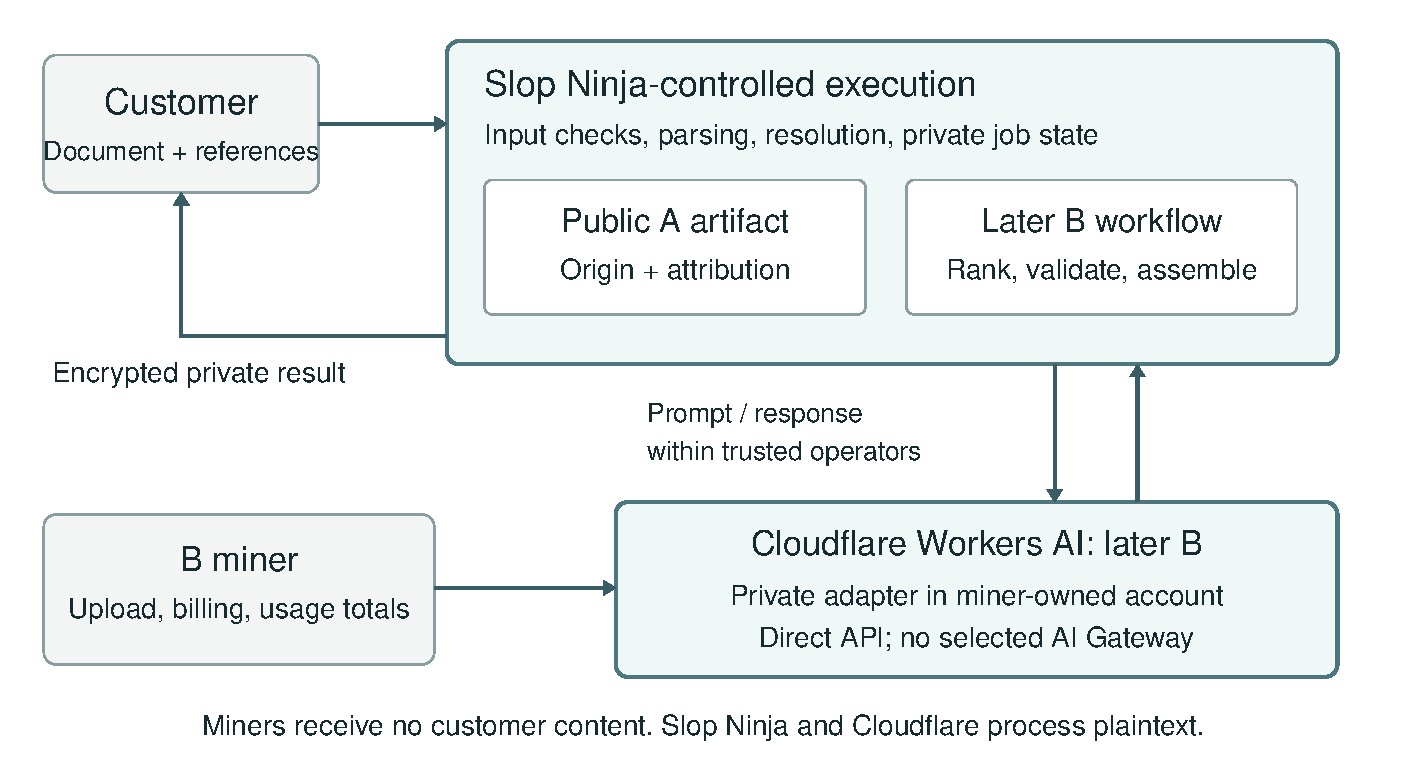
\includegraphics[width=\linewidth]{figures/private-inference.pdf}
\caption{Proposed customer execution paths. Public \textit{A} runs under SlopNinja's
control. Later \textit{B} uses a miner's billed Cloudflare account through direct
operator requests. Content isolation from that account's owner requires the
qualification described below; the diagram states the intended boundary.}
\end{figure}

\subsection{Direct serving and content logging}

The runtime sends synchronous calls to Cloudflare's direct Workers AI endpoint
for the enrolled account and base model, selecting the registered adapter UUID.
It omits AI Gateway selection, including the \texttt{cf-aig-gateway-id} header,
and accepts no miner endpoint, Worker, callback, or logging destination. It
forwards no caller-supplied routing headers and follows no redirects to miner
destinations. Provider-side batch jobs and stored conversations are excluded
because they may create additional owner-readable result surfaces. Cloudflare's
published data policy is an accepted provider assumption~\cite{cfdatausage};
the direct REST and gateway interfaces define different request
paths~\cite{cfdirectai,cfaigateway}.

The reported owner-session inspection on October 22, 2026 found aggregate usage
and no prompt or response text for the synthetic direct requests on the inspected
dashboard, audit, and observability surfaces~\cite{cfownerinspection}. The cited
record distinguishes that operator-supplied browser report from the direct API
checks, which also exposed per-request usage metadata. No AI Gateway existed
during those requests. This observation does not establish that an account
owner can never enable content capture. Before paid \textit{B} activation, run a controlled
comparison with gateway logging enabled: a routed positive control must appear,
and a direct request without gateway selection must remain unavailable. Examine
owner controls that could capture that direct request. Provider changes require
renewed qualification; absence from the surfaces inspected so far is limited
evidence, not a universal privacy proof.

Returned identity associates a response with the selected adapter under
Cloudflare's API behavior. It does not attest immutable weights or an unchanged
hosted base model. Enrollment checks private asset digests, updates receive
fresh version registrations and adapter UUIDs, and detected drift suspends
service. Periodic checks cannot exclude a change-and-restore race. Receipts state
the observed identity and enrolled digests without asserting a historical
measurement that the provider does not supply.

\subsection{Storage, isolation, and recovery}\label{assignment-recovery-and-the-privacy-boundary}

Customers submit over authenticated encrypted transport to SlopNinja. The
runtime processes plaintext, then encrypts the result to the customer's bound
output key for private retrieval. Private storage uses tenant authorization,
encryption, and declared retention. Operational logs contain identifiers,
usage, transitions, and normalized errors; provider errors must be sanitized
because they can echo a prompt. Content logging is disabled in Workers, traces,
and support tools. Profiles, vectors, intermediate candidates, and, for later
\textit{B}, parse trees and cached resolver outputs receive the same protection
as the original text. \textit{B}'s parsing and ambiguity resolution, including
any LLM resolver, run within the same SlopNinja and Cloudflare trust boundary;
miners receive neither resolver inputs nor outputs.

Each attempt binds its customer, job, assignment generation, model and pipeline
version, output key, and resource limits. State from one customer must not enter
another job. Recovery resumes only authorized durable state; reassignment
cannot silently introduce a new content recipient. A lost key or unavailable
result follows the job's failure and refund terms. Customer retention deadlines
remain in force during an evaluation pause. Preserving an unfinished benchmark
cohort indefinitely grants no authority to retain customer documents indefinitely.

Public receipts omit raw document hashes, filenames, titles, and report URLs.
Validator-accessible R2 inference receipts also exclude prompts, responses,
held-out labels, and parsed vectors. Their certified package and rolling
two-cohort deletion rule appear in Section~\ref{cohort-receipt-retention};
receipt access supplies no right to underlying content or commitment openings.
Content commitments use canonical encoding, a fresh secret salt, and separate
domains and lengths, for example:
\begin{equation}\label{eq:input-commitment}
C=\operatorname{SHA256}\bigl(
\mathrm{domain}\mathbin\Vert\mathrm{context}\mathbin\Vert
\mathrm{salt}\mathbin\Vert\mathrm{length}\mathbin\Vert
\mathrm{payload}\bigr).
\end{equation}
Salts and openings remain private. The context binds the deployment and job;
the output record also binds the customer's key and complete encrypted object's
digest and length. A commitment proves consistency when opened, not execution,
truth, or delivery. Result availability for the quoted retention period remains
an operator service obligation.

Model outputs are untrusted data. The runtime executes no generated tools,
URLs, or callbacks, and enforces schemas, budgets, and size limits. The result
viewer renders inert text without remote images or automatic link previews.
MCP delivery does not authorize commands embedded in a document. These controls
also apply to hostile source text and grammar contributions. An independent
security review before paid \textit{B} launch must test routing, credential
storage, content logging, cross-job isolation, and result access under this
provider-and-operator trust model.

A malicious adapter could encode prompt information in its output length,
exposing bits through owner-visible token counts or billed usage even when
content logging is disabled. Review must test this active channel and assess
fixed-size generation or output-size bucketing at the provider's metering
boundary. Padding the returned result cannot hide counts already metered by
the provider; a maximum output limit alone cannot close the channel. Ordinary
metadata visibility is accepted, but a demonstrated path to recover customer
content blocks paid \textit{B} activation until addressed. Mandatory traffic
padding is not otherwise part of the proposal, and passive metadata inference
remains a stated limit.

\subsection{Customer-directed disclosure}\label{customer-directed-evidence-disclosure}

A dispute gives validators no automatic right to read customer text. A customer
may authorize a separate disclosure naming the recipient, purpose, material,
and validity window. Further recipients require further authorization. Partial
evidence supports only a limited finding and cannot open a commitment to an
entire document. Expiry limits subsequent authorized processing but cannot
erase plaintext already received. Editorial review is advisory unless the
accepted service terms specify a remedy.

External detectors, including Pangram, receive customer content only with
separate authorization and funding. A service's benchmark record is not a live
external-detector result for the customer's document. Customer material enters
training only with separate opt-in; on-chain accounting and validator record
checks create no reuse exception.

\section{Paid inference, funding, and settlement}
\label{paid-asynchronous-jobs-and-on-chain-coordination}

The first commercial service is hosted \textit{A}: one admitted model returns
estimated AI share, AI-involvement confidence, and author
attribution within its qualified scope. Slop Ninja serves a published,
qualified artifact in its own infrastructure; \(R_0\) is such an artifact once
its public package is published
(Section~\ref{model-interfaces-and-starter-architectures}). Customers buy access through an API rather than
operating the artifact themselves. A later \textit{B} service would offer
bounded revision through private models hosted in miners' Cloudflare accounts,
under the conditions in Section~\ref{later-b}.

The coordinator opens paid inference only after deciding that measured quality
supports the advertised service. It publishes the accepted versions, supported
workloads, limitations, and activation decision. Emission eligibility alone
does not authorize a paid product. Each product needs its own cost,
availability, privacy, and delivery qualification; book-length inputs remain
outside an offer until those properties have been measured at that size.

Customer inference principal is converted to subnet alpha where needed and
burned. It pays neither a direct miner fee nor an operator margin. The economic
hypothesis is that customer demand purchases alpha where conversion is required
and removes alpha from supply through burns. Compared with retaining those
tokens, this may support alpha's market value for holders, including miners
and other emission recipients. It guarantees neither price appreciation nor
spendable proceeds sufficient to cover costs. This market-value channel is
distinct from a possible reward allocation for verified paid use, which
distributes emissions available under the chain's rules. Miners and the operator
must fund their bills while any emissions they earn remain subject to chain
allocation, market value, and liquidity.

The full-principal choice puts the entire inference price toward alpha burning,
purchasing alpha when conversion is required. The operator's intended upside comes
through its holdings and any owner or validator emissions it is entitled to
earn. This commits the treasury to funding operations and refund reserves
separately, accepting that exposure in pursuit of a benefit shared with other
alpha holders. The policy's commercial viability remains to be measured.

\subsection{Pricing and cost calibration}\label{market-pricing-in-alpha}

The operator quotes a fixed price for a bounded workload using a versioned
reference cost and multiplier:
\[
  P_{\mathrm{USD}} = M_{\mathrm{price}} C_{\mathrm{model}},\qquad
  C_{\mathrm{total}} = C_{\mathrm{model}} + C_{\mathrm{other}}.
\]
Here \(C_{\mathrm{model}}\) is the expected cost of all model invocations per
delivered job: execution of the \textit{A} artifact and, for later revision or a
later CFG input profile, ambiguity resolution, proposal, ranking, and required
semantic checks.
\(C_{\mathrm{other}}\) includes non-model parsing, orchestration, storage,
delivery, payment and chain fees, and expected refund overhead. Numeric-model
runtime is counted once. Training and mandatory benchmark research have
separate budgets.

An exploratory value is \(M_{\mathrm{price}}=25\). Detection and revision may need different
values. The multiplier sizes customer principal destined for burning relative
to reference model cost. Calibration must weigh the intended economic effect
against competitive pricing and customer demand. It does not set an operator
margin, fix the share of emissions allocated to inference, or guarantee a
miner's margin. Cost profiles bind model versions, workload limits,
maximum attempts, tariff assumptions, and measurement dates. Overruns cannot
increase an accepted quote. Repricing affects future reservations.

The initial detection hypothesis is \$0.02 per 1,000 words, with
\$0.01--\$0.03 as the first range to test. The following planning scenarios
are not measurements of a qualified production service.

\begin{center}
\small
\begin{tabularx}{\linewidth}{Lrrr}
\toprule
Service per 1,000 words & Model cost & Delivery subtotal & Price at \(M_{\mathrm{price}}=25\) \\
\midrule
Raw-text detection & \$0.0002875--\$0.0004250 & \$0.0004--\$0.0009 & \$0.007188--\$0.01063 \\
Bounded revision & \$0.008289 & \$0.0106--\$0.0112 & \$0.2072 \\
\bottomrule
\end{tabularx}
\end{center}

A launch detection job tokenizes the canonical text and runs the raw-text
\textit{A} artifact (Section~\ref{input-contract}); it has no grammar parse and
no language-model call. Its model cost is the October 29, 2026 Container
busy-time measurement, \$0.23--\$0.34 per 1,000 documents at the 2,048-token
limit, used as the bound for a 1,000-word document within that
limit~\cite{containerserving}. The bounded revision scenario, dated October 22,
2026, uses published tariffs and assumed workloads for later \textit{B}, which
parses its source~\cite{cfpricing}: 8,000 input and 1,000 output tokens of
batched ambiguity resolution on Llama 3.1 8B fast FP8, at \$0.045/\$0.384 per
million input/output tokens; three proposal calls totaling 12,000 input and
4,500 output tokens at the Mistral 7B v0.1 tariff of \$0.110/\$0.190; an
independent preservation check using 8,000 input and 600 output tokens at the
Llama 3.3 70B fast FP8 tariff of \$0.293/\$2.253; and \$0.00002 for numeric
scoring and ranking, an allocation that predates the Container measurement.
Both model costs include a 25\% failure/retry allowance. Prices use the
unrounded model-cost totals; model costs and prices are displayed to four
significant figures.

The delivery subtotal includes model cost and adds \$0.0001--\$0.0005 per
detection or \$0.0002--\$0.0008 per revision for orchestration, storage, and
delivery. Revision also assumes sixty seconds of non-model parsing and runtime
on a warm Cloudflare Container with one fully active vCPU, 6 GiB of memory, and
12 GB of disk, about \$0.00215 at the published resource
rates~\cite{cfcontainerspricing}. The subtotal excludes payment and chain fees,
refund reserves, training, evaluation, external checks, and low-volume fixed
costs. An idle Container of the standard-2 to standard-4 sizes costs
\$0.057--\$0.113 per hour, so idle capacity and cold starts can dominate per-job cost at low volume. Private-adapter
pricing remains uncertain beyond Cloudflare's advertised free LoRA beta; a
base-model tariff is only a comparison point~\cite{cfloras}.

The dated comparison uses Pangram's standalone realtime rate of \$0.50 per
1,000 words and its advertised bulk rate of \$0.40, against the proposed
\$0.02~\cite{pangrampricing,pangrambulk}. Subscriptions, negotiated prices,
per-item rounding, and differing detection performance limit this comparison.
Prices must be checked again when an offer is published. At
\(M_{\mathrm{price}}=25\), raw-text detection prices at about \$0.007--\$0.011,
at the bottom of the target range; a \$0.02 price corresponds to
\(M_{\mathrm{price}}\) of about 47--70. Price is an independent product
hypothesis, not evidence of comparable accuracy.

Calibration runs the whole admitted pipeline on authorized workloads at
realistic concurrency. Record every attempt's opaque identifier, model,
billed account, usage, latency, outcome, and tariff version without text.
Reconcile usage with provider charges, separating cash charges, promotional
credits, and undiscounted estimates. Divide the cost of all attempts by
successful deliveries, and report failures and cost percentiles separately.
Measure miner and operator expenses separately before selecting \(M_{\mathrm{price}}\), workload
limits, or a paid-use emission share.

\subsection{Checkout and the burn policy}

The planned funding routes are:
\[
\begin{aligned}
\text{USD card payment} &\longrightarrow \text{TAO}
  \longrightarrow \text{alpha} \longrightarrow \text{burn},\\
\text{TAO payment} &\longrightarrow \text{alpha}
  \longrightarrow \text{burn},\\
\text{alpha payment} &\longrightarrow \text{burn}.
\end{aligned}
\]
Coinbase Onramp is the selected candidate for card-to-native-TAO funding.
TAO.com's documented integration supports direct TAO delivery, but Slop
Ninja's access, supported card types and jurisdictions, recipient wallets,
limits, holds, and refunds still need qualification~\cite{coinbaseonramp}.
Credit-card support cannot be inferred from a documented debit-card flow.
This intended route requires neither Ethereum nor a separate bridge. Solana
is the preferred entry network for additional crypto inputs, pending a
qualified route to native TAO.

The target is automated checkout. Onramp delivery, conversion, service delivery,
and burning remain separate events with independent failure modes. Identity
checks, finality, and liquidity can delay them. A card authorization or an
expected exchange fill cannot fund execution; the adapter must confirm arrival
at the authorized funding destination. Provider-hosted forms handle card
details. Payment systems receive opaque job references, not customer documents
or author samples. At cent-scale prices, minimum purchases and fees may require
a funded balance spanning multiple jobs; that product rule remains open.

All inference principal follows the selected burn route. The operator funds
processing, conversion, and chain fees separately, including any shortfall
when a provider deducts fees from its output. Customers bear their own wallet
submission fees unless the offer explicitly sponsors them. Optional external
detector checks have a separate disclosed budget and require authorization to
send the text. Their charges neither reduce inference principal nor earn
additional inference credit.

A quote fixes the original currency and amount, conversion conditions, and
slippage limits. It records an estimated alpha quantity; the final record uses
actual fills and actual alpha destroyed. Native alpha's transfer and staking
semantics, deployment permissions, and burn operations must be qualified
against the runtime. Burning existing alpha does not itself buy TAO, and
recycling is a different operation~\cite{stakeburn,alphaburnimplementation}.
If the deployed burn call is owner-only, a subnet lease must provide an
authorized owner execution path or another verified route before sales open.
Operating the service does not itself grant that permission. This is separate
from the lease's required path for owner-controlled hyperparameter changes
(Section~\ref{participants-and-the-two-kinds-of-work}).
An address transfer or treasury allocation
alone cannot substantiate a burn claim.

Funds remain refundable custody until valid delivery and the published
pre-burn refund window have passed. Conversion may occur earlier if that
custody and its refund liability remain fully funded. Burn batches allocate
each job's principal uniquely and reconcile deposits, conversion fills,
custody, refunds, and finalized burns. Using treasury inventory temporarily
does not replace the promised purchase-and-burn accounting.

\subsection{Reservation, execution, and delivery}\label{reservation-and-delivery}
\label{application-and-agent-integration}

The API and an MCP integration expose quote, reserve, submit, status, and
result operations~\cite{mcp2026}. A quote binds the accepted pipeline and cost
profile, price and currency, input limits, attempt budget, acceptance and
delivery cutoffs, retention, and refund terms. Size and service requirements
suffice for discovery. The document goes to Slop Ninja only after reservation;
later \textit{B} miners receive no customer text through the discovery process.

\begin{enumerate}
\tightlist
\item Reserve confirmed funds, refund liquidity, and capacity durably before
dispatch. A customer idempotency key identifies one job. An expired or
exhausted offer cannot be reserved, and repricing cannot alter an existing
reservation. Cross-ledger operations must reconcile before execution.
\item Validate the submitted document, format, size, and customer output key
before acceptance. Construct the admitted input, canonical text under the
launch profile, and run the selected \textit{A} artifact. Check complete input
coverage, schema validity, probabilities, share/confidence consistency, and
attribution. An input beyond the artifact's length limit, or under a later CFG
profile an unresolved parse or exhausted ambiguity budget, produces an explicit
failure or a separately quoted diagnostic result.
\item For later \textit{B}, execute the bounded proposal and ranking procedure
and check the assembled document for preservation, readability, requested
tone, and any qualified author-fit objective. Local edit acceptance does not
establish whole-document success. Customer-requested Pangram checks require
separate disclosure authorization and funding.
\item Encrypt the result to the customer's output key, retain it in private
storage, and issue an operator-signed receipt. Retrieval must remain available
for the quoted period independently of a serving miner. Complete the required
delivery checks before authorizing burn or inference credit.
\item After the pre-burn window, settle the principal's burn allocation once.
Retain content-free accounting, return excess funds, and expire document data,
derived artifacts, and caches according to the disclosed retention policy,
including backup retention. Training reuse requires separate consent.
\end{enumerate}

The exact delivery predicate is a paid-launch prerequisite. It must bind a
durably stored encrypted object, the authorized customer/key, verified digest
and length, working retrieval, completed validations, and timely delivery.
Whether customer acknowledgment is required, and how acceptance interacts
with the refund window, remains to be fixed in the customer terms. A response
hash alone cannot authorize an irreversible burn. The offer buys a bounded
computation and retrievable result; subjective quality guarantees or additional
revision allowances require explicit terms.

Transactional Durable Object ledgers preserve reservations and transitions.
Queues carry job identifiers; private content stays in the operator account.
Persist each attempt's identity and maximum budget before dispatch. A timed-out
provider call may have executed and incurred charges, so mark its outcome
uncertain and reconcile before a bounded retry. Customer charges, burns, and
credits remain idempotent even when provider execution repeats. Restarts do
not extend accepted customer cutoffs. A cohort pause under
Section~\ref{cohorts} preserves research work but does not suspend delivery,
retrieval, or refund obligations.

Switching to another model or later \textit{B} provider requires either prior
customer authorization that fixes replacement eligibility and budget, or a
fresh quote and acceptance. A replacement cannot inherit the reserved model's
benchmark claim. Retain the original attempt and its outcome when a qualified
fallback completes the service.

\subsection{Receipts and refund liabilities}\label{receipt-certified-payment}
\label{payment-without-disclosing-the-job}

A completion receipt binds the protocol and chain domain, job and acceptance,
salted input commitment, customer output-key identity, enrolled model and
pipeline, attempt-ledger commitment, encrypted result digest and size,
deadline, and signer version. Linked payment records bind the quote,
original-currency amount, conversion history, and refund state. Burn records
bind finalized transactions and each job's allocation. Canonical encodings,
signature verification, key rotation, and replay protection must be fixed
before these records authorize funds.

Each inference attempt also has a content-free R2 receipt included in a certified
cohort package. Section~\ref{cohort-receipt-retention} defines its index, validator
verification, and deletion after two subsequent cohorts complete. That rolling
window applies to detailed inference receipts, separately from customer delivery
terms, compact burn/accounting records, and unresolved refund obligations.

Content-free commitments may be anchored on-chain, with inclusion proofs for
batches. Customer ciphertext, billing identity, report URLs, and raw document
hashes stay off-chain. Use fresh secret salts for document commitments. The
receipt states the operator's assertion about execution; it supplies neither
a Cloudflare signature nor independent validator certification. Result
availability remains an operator obligation. Later \textit{B} receipts report
the qualified identity evidence without claiming stronger historical model
immutability than the provider supports.

Rejection before acceptance releases funds and capacity. Failure to deliver
the agreed service requires the published refund; failed attempts still cost
the billed account holder and earn no inference credit. Valid delivery after
bounded retries keeps the original price. Cancellation after acceptance follows
the fixed terms. A conversion or burn delay retains pending credit and follows
its fixed cutoff. Reconcile finalized chain inclusion before deciding that
a pending transaction failed; a local timeout cannot both return principal
and leave an unresolved burn executable.

The proposed service refund restores the original amount in the original
currency: USD through a qualified return path, TAO to the bound refund address,
or alpha to its qualified position. Conversion losses and consumed provider
fees fall to the operator. Card checkout cannot promise this until an actual
USD return path is qualified; an onramp's completed crypto purchase may be
irreversible. Custodial intermediate alpha is reconciled into the refund,
not returned as an additional payment.

After a burn, a refund is a new operator-funded payment. Hold reserves for
retention obligations, service claims, and uncovered processor disputes;
reconcile chargebacks and manual refunds to avoid duplicate returns. Already
paid native emissions cannot be assumed recoverable. Stop new admissions when
required reserves are unavailable.

\subsection{Who pays, and what paid use earns}\label{revenue-and-costs}

Miners fund model preparation and training. Slop Ninja pays to serve public
\textit{A} artifacts, including their Container execution, storage,
coordination, and delivery. Later \textit{B} miners pay Cloudflare for their own customer
inference and bounded mandatory evaluation calls. They absorb permitted
failures and retries as part of participation. Their required candidate
Pangram reports use prepaid balances and a fixed budget; those deposits are
separate from burned customer principal. Unused, uncommitted balances remain
withdrawable.

The operator funds shared evaluation sets, source baselines,
authoritative \textit{A} execution, and independent review through named budgets.
Validators fund their own record verification and native weight submissions;
shared evaluation and service never depend on their funding or approval.
The operator also pays conversion and burn fees, refunds, and its other service
liabilities. Access to \texttt{rtao-rpc} has no service charge; transaction fees
and the caller's runtime costs remain. Insufficient evaluation funding reduces
new assignments rather than evidence requirements or accepted miner budgets.

These expenses require spendable operating funds. Customer principal is burned,
so a high markup supplies no cash for invoices. Capital or explicitly allocated
and realized owner proceeds may fund operations; future emissions are not
reserves. Native owner emissions accrue under the actual ownership or lease
arrangement and do not automatically fund Slop Ninja or an investor
\cite{mechanisms}. Report operating cash, purchased and burned alpha, miner
emissions, and separately priced enterprise services separately.

Section~\ref{benchmark-scoring-and-mechanism-mapping} defines the proposed
quality and paid-use allocations. Inference credit requires an admitted version,
acceptable delivery, and finalized allocation of paid principal to a burn.
Pending burns retain pending credit. Failed attempts, free traffic, mandatory
evaluations, duplicate receipts, and extra tokens earn none. Work units come
from a frozen workload schedule. A published \textit{A} artifact hosted by the
operator also requires an explicit choice about model-author credit versus
serving-cost credit before its calls enter a paid-use pool.

Assign usage to the epoch containing finalized burn inclusion plus a fixed
protocol lag. Publish that lag, the applicable emission-share schedule,
burn cutoff, and batch policy before admission. The operator cannot select
a favorable reward epoch after observing its pool. Delayed or late burns
follow the quoted resolution rule without creating duplicate principal
dispositions or retroactive work credit.

Section~\ref{token-economics} develops the burn hypothesis, cost-recovery
conditions, and self-purchase incentives. Its sensitivity analysis separates
miner participation from the operator's funding and reserve requirements.

\section{Token economics and capacity}\label{token-economics}

Paid demand, token value, miner rewards, and operating cash are separate
quantities. Their relationship determines whether the service can expand.
This section analyzes the proposed allocation before reward caps and native
consensus effects. It assumes no future alpha price and makes no claim that
the market will finance arbitrary inference volume. Checkout, delivery, burn
finality, and refund obligations follow
Section~\ref{paid-asynchronous-jobs-and-on-chain-coordination}. The analysis
applies once the mainnet subnet's alpha exists; revenue earned before
registration accrues in the pot of Section~\ref{testnet-revenue}, whose later
purchase and burn add to the burns analyzed here.

\subsection{What customer demand changes}

For \(N_{\mathrm{job}}\) identical delivered jobs priced at
\(P_{\mathrm{USD}}=M_{\mathrm{price}} C_{\mathrm{model}}\), the principal committed to burning is
\begin{equation}\label{eq:burn-principal}
 D_{\mathrm{burn}}=N_{\mathrm{job}} M_{\mathrm{price}} C_{\mathrm{model}}.
\end{equation}
Here \(D_{\mathrm{burn}}\) is a USD valuation of customer principal, not operating revenue.
For converted payments, if \(p_{\mathrm{buy}}\) is the realized USD-equivalent
purchase price per alpha, a planning approximation is
\(B_\alpha\approx D_{\mathrm{burn}}/p_{\mathrm{buy}}\). The ledger uses actual fills and
finalized destroyed alpha. Direct alpha payments already specify the quantity
to burn and need no new market purchase. Conversion fees and any shortfall
are separately funded under the full-principal policy.

Purchases create demand where conversion is needed; burns remove alpha that
would otherwise remain in supply. The intended benefit is support for token
value, including the value held or earned by miners, validators, and owners.
This is a market hypothesis. The reduction is relative to a counterfactual
without those burns. For total alpha supply under the deployed runtime,
the stock-flow accounting is
\[
 \Delta S_\alpha=\text{gross alpha minted}-\text{all alpha burned}.
\]
Any other supply-changing runtime operation must enter that reconciliation.
Concurrent issuance can still increase supply. Burned
alpha need not exceed emissions, and a burn does not establish net deflation,
price appreciation, or immediate liquidity. Chain allocation and market
responses can change together, so the analysis does not hold aggregate
emissions constant as a protocol fact.

The multiplier \(M_{\mathrm{price}}\) controls the principal removed for a given model-cost
estimate. It therefore trades off the intended economic effect against the
price customers will accept. It supplies no cash margin to the operator or
serving miner. A usage reward separately distributes available emissions;
the customer payment creates no direct claim to a share of its proceeds.

\subsection{Rewards per unit of work}

For one accounting period, let \(E_{\mathrm{miner}}\) be the miner-emission allocation in
alpha, \(f\) its paid-use share, and \(u_i\) participant \(i\)'s verified
paid-use work units. Write \(U_{\mathrm{paid}}=\sum_i u_i>0\). The intended uncapped reward is
\begin{equation}\label{eq:usage-economics}
\begin{gathered}
 R_i^{\mathrm{use}}=f E_{\mathrm{miner}}\frac{u_i}{U_{\mathrm{paid}}},\qquad
 V_{\mathrm{pool}}=f E_{\mathrm{miner}} p,\\
 \text{USD reward per work unit}=\frac{V_{\mathrm{pool}}}{U_{\mathrm{paid}}}.
\end{gathered}
\end{equation}
The parameter \(p\) is realizable USD per alpha after sale costs at the relevant
sale size and time. It differs from the purchase price
\(p_{\mathrm{buy}}\); liquidity, slippage, and timing can separate them.
The common \(p\) is a scenario input, not a guaranteed quote available to every
participant simultaneously. \(V_{\mathrm{pool}}\) is consequently the estimated realizable
value of the paid-use pool.

Equation~\ref{eq:mechanism-allocation} reserves \(c\) for later \textit{C},
\(f\) for paid \textit{A} use, and \(1-c-f\) for \textit{A} quality.
Increasing \(f\) reallocates this budget and can weaken the quality incentive;
it does not create additional emissions. \textit{C} starts at \(c=0\), and
paid service can operate with \(f=0\). Applying this arithmetic to later
\textit{B} requires its own approved reward and native-mechanism mapping.
Native normalization, consensus, and caps can change actual payouts from
\(R_i^{\mathrm{use}}\). A zero-work usage pool, one with no paid work in its
period, has no denominator; its treatment is fixed before the pool is enabled,
never by assigning invented work.

For an approved \textit{B} paid-use pool defined analogously, write its realizable
value as \(V_{\mathrm{pool}}\) for the following capacity calculation. For
homogeneous jobs, choose one work unit per job and let
\(C_b\) be the miner's variable cost per delivered job, including its permitted
failed attempts. Then the pool's average payout is \(V_{\mathrm{pool}}/N_{\mathrm{job}}\), and variable-cost
coverage requires
\begin{equation}\label{eq:inference-capacity}
 \frac{V_{\mathrm{pool}}}{N_{\mathrm{job}}}\ge C_b,\qquad N_{\mathrm{job}}\le\frac{V_{\mathrm{pool}}}{C_b}.
\end{equation}
Here \(N_{\mathrm{job}}\) counts jobs assigned to that reward period under the finalized-burn
and fixed-lag rule. Serving costs can fall due before those rewards are realized.
This is a necessary aggregate condition under proportional allocation.
Heterogeneous costs and unequal routing can leave individual miners below
break-even. Training, fixed capacity, mandatory evaluation, and required
external reports add further costs. Quality rewards may support those costs,
but an expected award is neither guaranteed reimbursement nor cash on hand.

Public \textit{A} has a different payer: SlopNinja serves the artifact and
pays the inference bill. Rewarding its author does not reimburse that bill.
Any split between author credit and serving-cost credit must be settled before
\textit{A} calls enter a nonzero paid-use pool. The same job cannot receive
two full units merely because its author and host differ.

\subsection{Pricing sensitivity and a scale example}

The planning costs in Section~\ref{market-pricing-in-alpha} are
\(C_{\mathrm{model}}=\$0.0002875\)--\(\$0.000425\) for raw-text detection and
\(\$0.0082885\) for revision per 1,000 words. At \(M_{\mathrm{price}}=25\), their
prices are \(\$0.0071875\)--\(\$0.010625\) and \(\$0.2072125\). The \(\$0.02\)
detection target instead implies \(M_{\mathrm{price}}\approx47\)--\(70\). For a
chosen price ceiling \(P_{\mathrm{USD,max}}\), the general constraint is
\(M_{\mathrm{price}}\le P_{\mathrm{USD,max}}/C_{\mathrm{model}}\).

The comparison of raw-text detection with Pangram's dated \(\$0.40\) bulk and
\(\$0.50\) realtime rates assumes neither equivalent accuracy nor equal terms.
Subscription discounts, minimum charges, and word-block rounding still apply.

\begin{figure}[!htb]
\centering
% Planning scenarios, USD per 1,000 words; no qualified production cost.
% Raw-text launch: 1.25 * Container busy time of $0.23--$0.34 per 1,000
%   documents at 2,048 tokens (measured 2026-10-29) = .0002875--.000425.
% Later CFG profile, 8B resolver: 1.25 * (8000 * .045 + 1000 * .384) / 1e6 + .00001.
% Later CFG profile, 70B resolver: 1.25 * (20000 * .293 + 2000 * 2.253) / 1e6 + .00001.
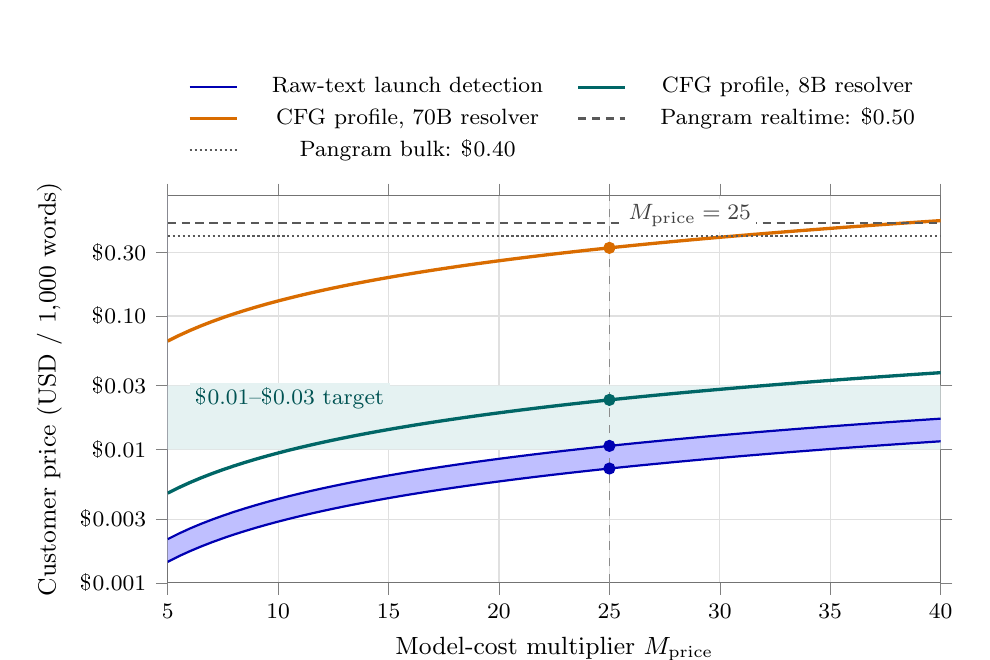
\begin{tikzpicture}
\begin{semilogyaxis}[
  width=.94\linewidth, height=6.5cm,
  xmin=5, xmax=40, ymin=.001, ymax=.8,
  xlabel={Model-cost multiplier \(M_{\mathrm{price}}\)},
  ylabel={Customer price (USD / 1,000 words)},
  xtick={5,10,15,20,25,30,35,40},
  ytick={.001,.003,.01,.03,.1,.3},
  yticklabels={\$0.001,\$0.003,\$0.01,\$0.03,\$0.10,\$0.30},
  minor y tick num=0,
  grid=major, grid style={black!12},
  tick align=outside, axis line style={black!55},
  font=\small, tick label style={font=\footnotesize},
  label style={font=\small},
  legend style={at={(.5,1.06)}, anchor=south, draw=none,
    font=\footnotesize, column sep=1em, /tikz/every even column/.append style={column sep=1em}},
  legend columns=2,
  clip=true,
]
\addplot[draw=none, fill=teal!10, forget plot]
  coordinates {(5,.01) (40,.01) (40,.03) (5,.03)} \closedcycle;
\addplot[draw=none, fill=blue!25, forget plot]
  coordinates {(5,0.0014375) (7.5,0.00215625) (10,0.002875) (12.5,0.00359375) (15,0.0043125) (17.5,0.00503125) (20,0.00575) (22.5,0.00646875) (25,0.0071875) (27.5,0.00790625) (30,0.008625) (32.5,0.00934375) (35,0.0100625) (37.5,0.01078125) (40,0.0115)
    (40,0.017) (37.5,0.0159375) (35,0.014875) (32.5,0.0138125) (30,0.01275) (27.5,0.0116875) (25,0.010625) (22.5,0.0095625) (20,0.0085) (17.5,0.0074375) (15,0.006375) (12.5,0.0053125) (10,0.00425) (7.5,0.0031875) (5,0.002125)} \closedcycle;
\addplot[blue!70!black, thick, domain=5:40, samples=71] {.000425*x};
\addlegendentry{Raw-text launch detection}
\addplot[blue!70!black, thick, domain=5:40, samples=71, forget plot] {.0002875*x};
\addplot[teal!80!black, very thick, domain=5:40, samples=71] {.00094*x};
\addlegendentry{CFG profile, 8B resolver}
\addplot[orange!85!black, very thick, domain=5:40, samples=71] {.0129675*x};
\addlegendentry{CFG profile, 70B resolver}
\addplot[black!65, densely dashed, thick] coordinates {(5,.50) (40,.50)};
\addlegendentry{Pangram realtime: \$0.50}
\addplot[black!65, densely dotted, thick] coordinates {(5,.40) (40,.40)};
\addlegendentry{Pangram bulk: \$0.40}
\addplot[black!45, dashed, forget plot] coordinates {(25,.001) (25,.8)};
\addplot[only marks, mark=*, mark size=2pt, blue!70!black, forget plot]
  coordinates {(25,.0071875) (25,.010625)};
\addplot[only marks, mark=*, mark size=2pt, teal!80!black, forget plot]
  coordinates {(25,.0235)};
\addplot[only marks, mark=*, mark size=2pt, orange!85!black, forget plot]
  coordinates {(25,.3241875)};
\node[anchor=north west, font=\footnotesize, text=black!75,
  fill=white, inner sep=2pt] at (axis cs:25.6,.76) {\(M_{\mathrm{price}}=25\)};
\node[anchor=west, font=\footnotesize, text=teal!65!black,
  fill=teal!10, inner sep=2pt] at (axis cs:6,.024) {\$0.01--\$0.03 target};
\end{semilogyaxis}
\end{tikzpicture}

\caption{Price sensitivity per 1,000-word detection job. The band spans the
raw-text cost of \$0.0002875--\$0.000425 from measured Container busy time,
including the stated retry allowance. The shaded \$0.01--\$0.03 range is the
proposed detection target; Pangram's dated bulk and realtime rates are price
comparisons only. The price axis is logarithmic. No token-price assumption
enters this calculation.}
\label{fig:pricing-sensitivity}
\end{figure}

The revision scenario assigns \(\$0.00271875\) per job to the miner's proposer
calls. Operator model, compute, storage, and delivery costs are approximately
\(\$0.0079\)--\(\$0.0085\). Raw-text detection's corresponding operator subtotal
is \(\$0.0004\)--\(\$0.0009\). Table~\ref{tab:tokenomics-volume} scales these
proxies without economies of scale. Burn principal is unavailable for either
party's bills.

Revision cost is sensitive to its resolver. The batched 8B resolution budget
costs \(\$0.00093\) after the retry allowance; a 70B resolver using 20,000 input
and 2,000 output tokens at the stated tariff would cost \(\$0.0129575\) instead,
raising revision model cost from \(\$0.0082885\) to \(\$0.020316\), about
\(\$0.5079\) at \(M_{\mathrm{price}}=25\). For such workloads the escalation
rate and workload bounds matter more than the multiplier.

\begin{table}[htbp]
\centering\small
\begin{tabularx}{\linewidth}{Lrrrr}
\toprule
Service & Jobs & Burn principal & Miner serving & Operator delivery \\
\midrule
Detection & 1,000 & \$7.19--\$10.63 & --- & \$0.39--\$0.93 \\
Detection & 100,000 & \$719--\$1,063 & --- & \$39--\$93 \\
Revision & 1,000 & \$207.21 & \$2.72 & \$7.90--\$8.50 \\
Revision & 100,000 & \$20,721.25 & \$271.88 & \$790--\$850 \\
\bottomrule
\end{tabularx}
\caption{Illustrative period totals at \(M_{\mathrm{price}}=25\) for 1,000-word jobs, rounded
for display. Serving costs use tariff proxies, the synthetic-text Container
measurement, and assumed retry/runtime budgets, not production measurements. They exclude payment and chain fees,
refund reserves, training, evaluation, external checks, and low-volume fixed
costs. Public \textit{A} has no miner serving charge in this architecture.}
\label{tab:tokenomics-volume}
\end{table}

\subsection{Capacity and operating reserves}

If volume grows by a factor \(k\) while per-job cost stays unchanged, \(V_{\mathrm{pool}}\)
must also grow by at least \(k\) to preserve the same reward per job. The average
log elasticity over that change must therefore be at least one.
Purchase-and-burn establishes no law forcing this response:
\(f\), \(E_{\mathrm{miner}}\), and realizable \(p\) may each remain flat or fall. With a fixed
pool, doubling volume halves the reward per unit. Equation~\ref{eq:inference-capacity}
then gives a budget-dependent serving limit, not unlimited scalability.

\begin{figure}[htbp]
\centering
% Homogeneous bounded-revision planning scenario. Each job is 1,000 words.
% Cash costs and burned principal are distinct flows, all expressed in USD.
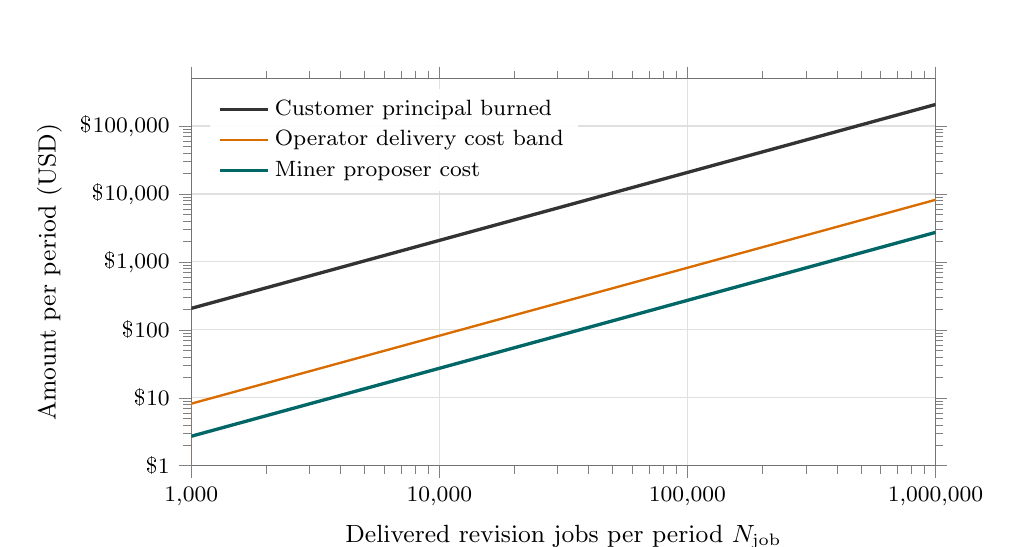
\begin{tikzpicture}
\begin{loglogaxis}[
  width=.91\linewidth, height=6.5cm,
  xmin=1000, xmax=1000000, ymin=1, ymax=500000,
  xlabel={Delivered revision jobs per period \(N_{\mathrm{job}}\)},
  ylabel={Amount per period (USD)},
  xtick={1000,10000,100000,1000000},
  xticklabels={{1,000},{10,000},{100,000},{1,000,000}},
  ytick={1,10,100,1000,10000,100000},
  yticklabels={\$1,\$10,\$100,{\$1,000},{\$10,000},{\$100,000}},
  minor x tick num=0, minor y tick num=0,
  grid=major, grid style={black!12},
  tick align=outside, axis line style={black!55},
  font=\small, tick label style={font=\footnotesize},
  label style={font=\small},
  legend style={at={(.025,.975)}, anchor=north west, draw=none,
    fill=white, fill opacity=.95, text opacity=1, font=\footnotesize,
    cells={anchor=west}},
  clip=true,
]
\addplot[black!80, very thick, domain=1000:1000000, samples=2] {.2072125*x};
\addlegendentry{Customer principal burned}
\addplot[draw=none, fill=orange!60, forget plot]
  coordinates {(1000,7.9) (1000000,7900) (1000000,8500) (1000,8.5)} \closedcycle;
\addplot[orange!85!black, thick, domain=1000:1000000, samples=2] {.0082*x};
\addlegendentry{Operator delivery cost band}
\addplot[teal!80!black, very thick, domain=1000:1000000, samples=2] {.00271875*x};
\addlegendentry{Miner proposer cost}
\end{loglogaxis}
\end{tikzpicture}

\caption{Revision totals versus delivered 1,000-word jobs in one period.
Burn principal is \$0.2072125 per job; miner proposer cost is \$0.00271875;
operator delivery costs span \$0.0079--\$0.0085. Both axes are logarithmic.
The curves scale fixed planning assumptions and exclude the additional costs
listed in Table~\ref{tab:tokenomics-volume}. The burn curve is not a funding
source, and no alpha price or emission trajectory is forecast.}
\label{fig:volume-sensitivity}
\end{figure}

Operator solvency needs its own constraint. Let \(T_{\mathrm{cash}}\) be available treasury
cash excluding customer custody, \(F_{\mathrm{cash}}\) additional realized operating funding,
\(O_{\mathrm{due}}\) service and shared expenses due, \(L_{\mathrm{due}}\) refunds and other liabilities
due, and \(H_{\mathrm{reserve}}\) the required reserve for remaining future obligations. Admission
must preserve
\[
 T_{\mathrm{cash}}+F_{\mathrm{cash}}-O_{\mathrm{due}}-L_{\mathrm{due}}\ge H_{\mathrm{reserve}}.
\]
No term includes burned principal. Capital or explicitly allocated, realized
owner proceeds can contribute to \(F_{\mathrm{cash}}\); future emissions cannot. Native owner
entitlement follows the ownership or lease arrangement and does not itself
entitle SlopNinja or an investor to those proceeds. Reserves must also match
the currencies and timing of liabilities, so a USD-equivalent surplus alone
does not establish that refunds can be paid.

\subsection{Self-purchases and low-volume rewards}

Burning gives artificial demand a cost, but a large pool divided among little
legitimate work can still reward it. Let \(U_{\mathrm{honest}}>0\) be existing legitimate
work, \(u_{\mathrm{self}}\) additional self-purchased work credited to an attacker, and \(k_s\)
the attacker's incremental cost per such unit, including the full customer
price and its own variable serving costs. For an attacker with no preexisting
share, holding \(V_{\mathrm{pool}}\) fixed gives the simplified gain
\begin{equation}\label{eq:self-purchase-gain}
 \Pi(u_{\mathrm{self}})=V_{\mathrm{pool}}\frac{u_{\mathrm{self}}}{U_{\mathrm{honest}}+u_{\mathrm{self}}}-k_s u_{\mathrm{self}}.
\end{equation}
This assumes the attacker can route the purchases to its own credited model.
If it already earns \(V_{\mathrm{pool}} u_a/U_{\mathrm{honest}}\) from legitimate work, measure incremental
gain instead:
\[
 \Delta\Pi(u_{\mathrm{self}})=V_{\mathrm{pool}}\left(\frac{u_a+u_{\mathrm{self}}}{U_{\mathrm{honest}}+u_{\mathrm{self}}}-\frac{u_a}{U_{\mathrm{honest}}}\right)-k_s u_{\mathrm{self}}.
\]
Existing rewards are not new attack proceeds. Both expressions omit caps,
price feedback, quality-reward changes, and other controlled identities.

\begin{figure}[htbp]
\centering
% Hypothetical fixed reward pool V_{\mathrm{pool}}, honest work U_{\mathrm{honest}} > 0, no prior attacker work.
% r_self = u_self / U_honest; a = full self-purchase cost per work * U_honest / V_pool.
% Normalized incremental payoff is r_self/(1+r_self) - a*r_self.
% PGFPlots' internal variable x represents r_self. No token-price forecast.
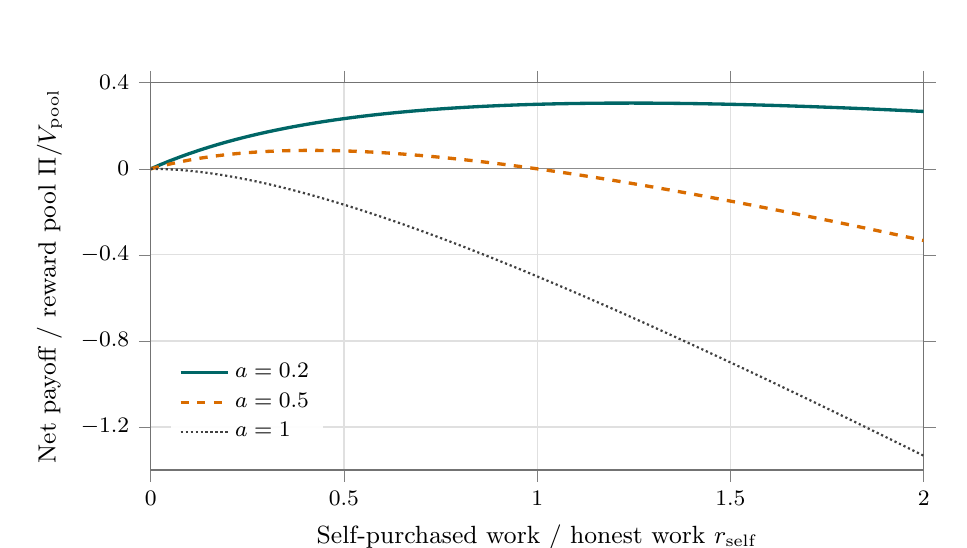
\begin{tikzpicture}
\begin{axis}[
  width=.94\linewidth, height=6.5cm,
  xmin=0, xmax=2, ymin=-1.4, ymax=.4,
  xlabel={Self-purchased work / honest work \(r_{\mathrm{self}}\)},
  ylabel={Net payoff / reward pool \(\Pi/V_{\mathrm{pool}}\)},
  xtick={0,.5,1,1.5,2},
  ytick={-1.2,-.8,-.4,0,.4},
  grid=major, grid style={black!12},
  tick align=outside, axis line style={black!55},
  font=\small, tick label style={font=\footnotesize},
  label style={font=\small},
  legend style={at={(.025,.045)}, anchor=south west, draw=none,
    fill=white, fill opacity=.95, text opacity=1, font=\footnotesize,
    cells={anchor=west}},
  clip=true,
]
\addplot[black!45, thin, forget plot] coordinates {(0,0) (2,0)};
\addplot[teal!80!black, very thick, domain=0:2, samples=81] {x/(1+x)-.2*x};
\addlegendentry{\(a=0.2\)}
\addplot[orange!85!black, very thick, dashed, domain=0:2, samples=81] {x/(1+x)-.5*x};
\addlegendentry{\(a=0.5\)}
\addplot[black!75, thick, densely dotted, domain=0:2, samples=81] {x/(1+x)-x};
\addlegendentry{\(a=1\)}
\end{axis}
\end{tikzpicture}

\caption{Simplified self-purchase incentive with fixed \(V_{\mathrm{pool}}>0\), honest
traffic \(U_{\mathrm{honest}}>0\), no preexisting attacker credit, and no reward cap. Set
\(r_{\mathrm{self}}=u_{\mathrm{self}}/U_{\mathrm{honest}}\) and \(a=k_s U_{\mathrm{honest}}/V_{\mathrm{pool}}\); normalized gain is
\(\Pi/V_{\mathrm{pool}}=r_{\mathrm{self}}/(1+r_{\mathrm{self}})-a r_{\mathrm{self}}\). Curves vary the cost of buying work relative to the
pool. They are sensitivity cases, not measured attack profitability.}
\label{fig:self-purchase-sensitivity}
\end{figure}

With no preexisting attacker credit, the initial marginal gain is positive
when \(V_{\mathrm{pool}}/U_{\mathrm{honest}}>k_s\). With no honest
work, any positive sole credited purchase can capture the entire uncapped
pool. A cap on work units or on one identity's share does not solve this after
renormalization or identity splitting. Qualification needs an absolute cap on
released rewards relative to attributable paid burn, applied across common
control and the total pool, with an explicit destination for unused allocation.
No numerical cap or implementation is selected here. Validator dividends,
owner proceeds, and other rewards under common control must enter the combined
attack budget; a miner-only calculation cannot establish resistance.

\subsection{Calibration and activation decisions}

Low demand makes reward concentration and fixed costs more important; high
demand raises aggregate bills and can dilute rewards below serving cost.
Calibration must test both regimes, including declining realizable token value,
illiquid sales, resolver escalation in later \textit{B}'s parsed workloads, retry spikes, provider repricing,
delayed burns, and post-burn refunds. Use measured cost distributions rather
than only averages, and treat free beta inference as a temporary subsidy.

Before enabling a paid-use pool, fix workload credit, author-versus-serving
credit, \(f\), release caps, zero-work pool treatment, and the native payout mapping.
Choose \(M_{\mathrm{price}}\) against measured quality, customer prices, and operating capacity;
fund reserves before accepting liabilities. Update offers and future reward
schedules through their published versioning rules. Rising burns or demand
alone do not justify raising capacity beyond funded obligations and miners'
willingness to serve.

\section{Later transformation mechanism}\label{later-b}\label{reward-adjudication}

\textit{B} is a later mechanism for authorized revision toward a requested
writer's voice, with preserved meaning and measured resistance to origin
detectors. Its activation requires a separate scoring-authority decision,
editorial validation, serving qualification, and reward allocation. The
coordinator-led \textit{A} pilot does not settle who adjudicates \textit{B}'s
semantic disputes. This section retains a candidate evaluation design; its
formulas and service gates are not active launch rules.

\subsection{The editing task}\label{author-transformation-and-detector-evasion}

A benchmark supplies source text, independent authorized target-author samples,
and a brief fixing the requested style and preservation requirements. Sources
may have human-only, model-only, or mixed production histories. Revision
preserves source ancestry while extending the candidate's production history:
a model revision of human-only text is mixed under the initial labeling policy.
Intended uses include editing one's own or licensed
writing and authorized detector research; a low detector score cannot cancel
disclosure obligations attached to the eventual use.
The private job record binds the authenticated requester, source and reference
identities, declared permission to submit and transform them, and relevant
license or permission records where applicable. These records document the
authorization basis; a declaration alone cannot establish ownership.

Matching a writer includes lexical, grammatical, and rhetorical habits in the
requested register. The brief distinguishes unwanted filler and repetition from
deliberate informality and idiosyncrasy. It may request a different tone from
the source. Without such a direction, source tone supplies the default.
Shortening, simplification, and stronger rhetoric count as improvements only
when they serve the brief without losing information or increasing certainty.

For the main intended customer workflow, the target is the private writer
profile built from the user's samples (Section~\ref{author-and-origin-detection}).
The shared English CFG is the proposed pipeline's edit representation: it
divides the source into word, phrase, and clause units, types each proposed
edit, and reparses candidates so a revision can be compared with its source.
\textit{A}'s continuous author-fit signal against that profile ranks successive
revisions; grammar-level writer-style features are a candidate further input to
that guidance, qualified on their own evidence. The
categorical \emph{Provided writer} match alone is too coarse to guide this
search. No representation tested so far supplies that signal: rewrites toward a
target writer scored near chance against rewrites toward other writers for
encoder, stylometric, CFG, and fused profiles alike, and the kind of rewrite
moved scores more than the target voice did (Section~\ref{writer-profile-evidence}).
The feedback therefore waits for the learned matcher's qualification and for
rewrites conditioned on several of a writer's own samples, data that does not
exist yet. Freeze the reference profile, \textit{A} artifact, and calibration
for the job so an apparent improvement cannot come from changing the target.
A language model may propose changes within the registered procedure; the
private ranker receives compatible source and candidate bundles, deltas, the
writer profile, and declared task controls. The target-style input is the
profile rather than raw reference writing. Source prose remains available to the
authorized editing runtime, and trusted preprocessing still reads the samples.
Neither samples nor profiles enter a miner-accessible request path. Candidate
selection retains separate meaning, readability, and tone checks; a higher fit
score cannot erase a revision's production history.
Whether the grammar's typed edits and this profile support useful transformation
remains an empirical question. Private serving and the provider/operator trust boundary are specified
in Section~\ref{confidential-customer-inference}.

The assembled document is the evaluation unit. Later qualification must cover
multi-paragraph work and, for profiles advertised to support them, complete
manuscripts and books. Context windows and local edits are implementation
units. Evaluation retains every span and checks cross-section claims,
terminology, attribution, and voice. A chapter or sentence score cannot certify
the complete work. Each length class needs measured resource limits,
failure behavior, and whole-document quality evidence.

\subsection{A frozen comparison}\label{common-transformation-evidence}

Before generation, the evaluation authority freezes the service version,
workload profile, task population, references, style evaluator, detector panel,
source baselines, and funded evidence budget. The benchmark uses the same
bounded pipeline offered to customers. Its profile limits internal attempts,
context, output, search, and cost. Each invocation produces one final candidate
or abstention; all attempts and recovery actions remain recorded. Cloudflare
generation may vary between runs, so qualification measures variability without
claiming identical-output replay.

The proposed panel uses three qualified, distinct \textit{A} inference
artifacts: the prior-round origin leader and two preselected members. Before
activation, choose whether the leader is ranked by binary AI-involvement Brier
score or three-class origin Brier score. That choice is separate from
\textit{A}'s quality anchor and reward baseline. Freeze reserves before issue;
after issue, recovery executes the same judges. Miners cannot nominate the
panel, benchmark inputs, or a replacement comparison. Too few competitive
artifacts require separately reported, funded bootstrap comparisons.

Run the complete source/candidate matrix under the frozen parsing, resolution,
projection, and execution contracts. Retain the strongest detector's result
separately. Miner self-scores remain nonauthoritative. Distinct artifacts and
UIDs do not establish independent ownership; collusion and candidate-triggered
errors belong in qualification tests. \textit{A} earns quality credit against
independent production-history labels, so judging \textit{B} harshly supplies
no reward by itself. Hidden labels and unreleased review material remain with
authorized evaluators; retired examples need authorization before release.

\paragraph{Accepted bytes.}\label{canonical-text-profile}
The English benchmark profile specifies UTF-8, NFC, LF-only endings,
permitted scripts and code points, and pinned Unicode/security-data versions
with test vectors~\cite{unicodenormalization,unicodesecurity}. It forbids a
terminal LF, BOM, undeclared invisible or bidirectional controls, tabs, edge
whitespace, repeated spaces, and excess blank lines. Predeclared literal spans
receive only exact-copy whitespace exceptions; they cannot add a terminal LF.
Sources, references, and briefs conform before issue. Other formatting requires
an explicitly qualified profile.

The runtime may finalize an uncommitted draft inside its measured procedure.
Signed text is never silently repaired. Receipts, commitments, reconstructed
vectors, style evaluation, reviewer display, and authorized Pangram requests
bind identical accepted bytes. Decode the provider's returned analyzed text
and compare its UTF-8 bytes exactly; a changed copy is unusable evidence.
The probe behind the terminal-LF restriction and its limitations are recorded
in Section~\ref{audit-sequence}. Qualify supported report retrieval and retention
before live use. Report URLs may expose text and stay out of public receipts
and logs. Customer disclosure to Pangram requires separate permission.

\subsection{Style, preservation, and detector improvement}
\label{preservation-before-revision-rewards}
\label{transformation-and-improvement-utility}

The public style evaluator is frozen independently of the private ranker. Its
contract binds the profile schema, feature meanings, reference pooling,
parameters, executable, numerical operations, rounding, and resource bounds.
For text \(t\) and reference set \(\mathrm{Refs}\), it returns a nonnegative
integer distance \(d_\theta(t,\mathrm{Refs})\). Under the proposed personal-profile
workflow, \(\mathrm{Refs}\) binds the writer profile and its construction
record; evaluating a candidate requires no raw reference prose. A qualified
\textit{A}-derived author-fit distance is the intended implementation. Its
mapping to this integer distance and its calibration must be fixed and tested
before use; a categorical match or an uncalibrated similarity cannot replace
the evaluator. A nonempty calibration multiset
\((c_1,\ldots,c_M)\) contains distances from development queries to independent
same-author reference work; source families are separated from fitting and
evaluation. Duplicate values remain. With \(Q=1{,}000{,}000\), define
\begin{equation}\label{eq:style-fit}
 q(t,\mathrm{Refs})=\left\lfloor
 Q\,\frac{2\#\{m:c_m>d_\theta(t,\mathrm{Refs})\}
             +\#\{m:c_m=d_\theta(t,\mathrm{Refs})\}}{2M}
 \right\rfloor.
\end{equation}
Ties receive half credit. This rank supplies neither authorship probability nor
semantic approval. Source \(x\) and candidate \(z\) share references and
calibration, giving \(q_x,q_z\). Positive style improvement uses remaining
headroom:
\begin{equation}\label{eq:style-utility}
 V(x,z)=\begin{cases}
 0,&q_x=Q,\\
 \displaystyle\frac{\max(0,q_z-q_x)}{Q-q_x},&q_x<Q.
 \end{cases}
\end{equation}
Keep exact rational values through aggregation and check raw nonregression
\(q_z\geq q_x\) separately. A tie or already-maximal source earns no invented
improvement. Before rewards depend on this evaluator, test adaptive searches
that optimize it through reference copying, topic substitution, omissions,
padding, or changes of meaning. Among semantically acceptable candidates,
higher rank must also agree with independent judgments of author fit.

Readers inspect the complete source and candidate before seeing numerical
scores. The frozen rubric has three fields:
\begin{itemize}
\tightlist
\item \(P\), preservation of complete meaning: claims, entities, quantities,
negation, uncertainty, citations, attribution, and argument relations. Review
covers omissions from the checklist as well as listed facts. Unsupported
additions and stronger factual certainty fail.
\item \(R\), readability without material regression, including requested
cleanup of filler or formulaic phrasing. Brevity alone earns no approval.
\item \(T\), the requested tone and audience constraints, preserving deliberate
voice features. This field still applies when source tone supplies the default.
\end{itemize}
Every field records pass, fail, or unresolved with reasons. Set \(G=1\) only
after all required approvals; an established failure gives \(G=0\). Missing
evidence leaves \(G\) unknown. An automated judge needs validation against
separate readers before influencing rewards. Controls include unchanged
sources, qualified human edits, fluent semantic errors, erased voice, and
detector-passing revisions that retain unwanted habits. Instructions inside
evaluated prose are data. Blinded reader studies must have enough power for
the claims made about voice and quality.

Pangram's reported AI-plus-assisted fraction \(F_r(t)\) differs from a
document-level probability of AI involvement~\cite{pangramapi}. Retaining the
three-observation proposal for each source and candidate gives
\begin{equation}\label{eq:evasion-improvement}
 \Delta_P(x,z)=\min_r F_r(x)-\max_r F_r(z).
\end{equation}
Reopening one report does not create another observation. The coordinator
binds report counts, request identities, repetition/retry rules, provider
version, and usable evidence before generation. All required observations and
failures remain in the ledger; neither miner nor operator may select favorable
reports after seeing scores. Retry and provider-drift rules need qualification
before activation. The operator funds shared source observations; miners fund
their bounded candidate observations and evaluation inference as participation
costs. Section~\ref{audit-sequence} reports the limited repeatability evidence.

For panel member \(j\), let \(H_j(t)\) be its frozen AI-involvement probability
and \(\Delta_j=H_j(x)-H_j(z)\). Define
\(\Delta_S=\operatorname{median}_{j=1}^{3}\Delta_j\), retaining every raw
answer. The provisional joint detector improvement is
\begin{equation}\label{eq:joint-evasion-utility}
 E(x,z)=\begin{cases}
 (\Delta_P+\Delta_S)/2,&\Delta_P\geq0\ \text{and}\ \Delta_S\geq0,\\
 0,&\text{otherwise}.
 \end{cases}
\end{equation}
With complete evidence, the candidate utility is
\begin{equation}\label{eq:transformation-utility}
 U_B(x,z)=\begin{cases}
 G(V+E)/2,&q_z\geq q_x,\ \Delta_P\geq0,\ \Delta_S\geq0,\\
 0,&\text{otherwise}.
 \end{cases}
\end{equation}
These weights remain a proposal requiring reader validation and an allocation
decision. Each comparison measures both objectives. One component can improve
while others hold steady; a clipped value cannot hide regression.

Strict detector success additionally requires every candidate Pangram fraction
below 10\%, a majority of panel members below their independently calibrated
human-false-positive thresholds, and a pass at the prior-round leader's own
threshold. It also requires the approvals and raw nonregression checks above.
Incremental utility can be positive before this target is reached. Reports
separate utility, author fit, each detector result, and strict success. A zero
source Pangram baseline permits no candidate increase, although approved style
improvement can still earn utility. Each candidate's label follows its complete
production workflow, regardless of detector scores.

For detection customers, a successful evasion is a false negative by the
affected \textit{A} detector. Its reported limitations must include performance
on held-out revisions from evaluated \textit{B} pipelines. Such revisions can
expose weaknesses for future training, but only fresh evaluation can establish
an improvement in detection.

Reducing required Pangram checks later needs repeated held-out noninferiority
studies, including new adversarial revisions and difficult human slices.
Calibrate the fraction and probability outputs to the same independently
labelled event on separate development data. Agreement with Pangram or a
change of quality anchor is insufficient. A reduced-check policy must state
how unchecked candidates are scored and how provider drift is detected.

\subsection{Service and outcome accounting}\label{service-evidence}
\label{adversarial-feedback-loop}

Later mandatory training service has separate \textit{A}-requester and
\textit{B}-provider classes. No such duties apply to the \textit{A}-only launch.
Before issue, reserve shared evaluation resources, candidate-report funding,
and the provider's accepted inference budget. The requester pays no extra
service price; the provider absorbs its participation costs for potential
emissions. Publication and qualification of \textit{A} remain separate.

A durable ticket binds registration generations, service versions, task and
capacity limits, ordered counterparties, and feasible response windows.
Assignments consume permanent slots; callers cannot nominate peers, redraw by
declining, or turn retries into new quota. A valid admitted request activates
provider responsibility. Fallback success preserves earlier failure.
Unresolved validity stops dependent attempts. Keys, UID reuse, migrations, and
restarts cannot silently reset counters or remove outstanding work.
Coordinator outages preserve the cohort and evidence under the recovery
protocol; elapsed wall time alone cannot erase an obligation.

For each applicable service class, retain
\(O_{\mathrm{act}}=S+F+U+O_{\mathrm{void}}\): successes, attributable failures,
unresolved cases, and scoped voids. Unused reservations stay separate. The
proposed availability rule requires \(U=0\), \(N=S+F>0\), and
\(10F\leq N\), plus qualification and a cleared deficit
\(D_e=\max(0,D_{e-1}+10F-N)\). Recovery work belongs to the failed class;
customer volume, voids, and unresolved work cannot repay that deficit. A
compliant abstention can satisfy delivery while earning no quality improvement.
No inactive class needs an artificial empty success.

Benchmark closure distinguishes missing or unscorable candidates, unresolved
judgments, and scoped platform failures. Under the proposed accounting rule, these
slots earn zero and keep their assigned denominator weight and actual status.
One uncertain candidate cannot erase completed competitors. Shared treatment
requires evidence of a common cause and applies uniformly to its declared
scope. Semantic uncertainty alone does not prove an assigned-service failure.
Provider revocation, deletion, exhausted billing, or unreserved concurrent use
can establish provider fault only through the adopted attribution procedure.

Before \textit{B} activates, choose its review authority, evidence access,
incident deadlines, appeals, and correction rules. Other validators' approval
or availability cannot gate review, closure, or service; their only protocol
dependency is timely submission of the prescribed native weight rows.
Reserve capacity for complete review and qualify these rules against outages
and strategic withholding. Preserve signed decisions and attempt records through
recovery; coordinator records cannot claw back native emissions already
distributed.

\section{Later mechanism C: grammar contributions}\label{grammar-contributions}

\textit{C} would reward improvements to the shared English CFG and lexicon.
It starts inactive. Its objective is correct, reusable analysis of English as
used, including informal constructions, unusual vocabulary, spelling errors,
and embedded technical or foreign material. It must not equate prescriptive
correctness with parseability or reward broad catch-all rules merely for
accepting more text.

A candidate round accepts bounded public patches against one fixed parent
profile. Contributions may add lexical forms and parts of speech, structural
productions, or a more accurate analysis of text already covered. Examples must
be authorized for that use. The coordinator reviews the linguistic claims,
measures transfer to held-out documents, replays affected earlier analyses, and
checks interactions among accepted proposals. A changed old parse deserves
inspection; change alone is not a regression. Whole-document coverage, quality
of the interpretation, remaining ambiguity, and resource cost are separate
measurements.

The central coverage statistic is the fraction of requested documents with
complete accepted analyses. A parser accepting every token is weaker evidence
than an analysis whose structural decisions have been checked. Report both,
retain failures in the requested population, and track initial coverage on new
documents before any repair. Freeze resource limits so a gain cannot come solely
from lifting a ceiling. Rule count, added bytes, dictionary size, and grammar
size are not reward scores.

Accepted changes enter a subsequent shared profile. The launch \textit{A}
comparison reads raw text and does not depend on it; any comparison that uses a
CFG input profile continues with its frozen grammar, projection, and selected
derivations.
Compact cached parses and production dependencies reduce repeated work, but
new productions can affect documents outside the old dependency set. The
acceptance protocol therefore needs both targeted replay and broader change
detection. Changes in feature meaning require requalification; retaining a
profile name cannot hide a new representation.

Each accepted contribution earns credit once. A durable contribution identity
and credited recipient prevent a later release, continued use, or resubmission
from earning a second award. Before activation, define overlapping-proposal
credit, interaction failures, regressions, award size, settlement epoch, and
when a credited contribution stops influencing native weights. Repeatedly
leaving the same credited contribution in a live reward row would defeat the
one-time rule. A scored pilot without payouts can test those decisions before
assigning a nonzero \(c\) in Equation~\ref{eq:mechanism-allocation}.

The project already develops its grammar as research infrastructure. That work
does not establish a live \textit{C} protocol, and a \textit{C} award would not
itself establish improved detection. The downstream model comparison must test
whether a new shared representation improves quality enough to justify its
parsing and resolution cost.

\section{External comparisons and evidence renewal}\label{pangram-evidence-and-assigned-audits}

Pangram begins as the external origin-quality anchor: the designated comparator
for claims of competitive detection quality and the coordinator's assessment
of readiness for paid service. It supplies a reference for those decisions;
commercial activation still follows the workload-specific criteria in
Section~\ref{development-and-launch-criteria}. The coordinator compares
qualified \textit{A} artifacts, the incumbent anchor, and Pangram on the same
hidden, independently labeled population. Shared provider observations are
funded once per comparison set; admitting another artifact need not
multiply that bill. Freeze provider/model versions, repetition policy, population
weights, operating points, and uncertainty analysis before exposing the set.
Rotate private sources, track repeated use, and release material only after
retirement and source authorization.

Pangram reports separate fractions classified as AI-generated, AI-assisted,
and human, with segment confidence reported separately~\cite{pangramapi,pangramcard}.
Its current dashboard explanation defines the fractions by character count;
our share target uses final-word counts in recorded model-produced spans~\cite{pangramscores}.
Both are distinct from \textit{A}'s probability of any document-level involvement.
Quantitative share comparisons need common span labels and counting units;
the raw fractions are not interchangeable.
Compare both against documented histories at independently calibrated operating
points. Provider agreement supplies neither ground-truth labels nor reward
credit. The reference model that serves as the reward baseline, the
external quality anchor, and the later \textit{B} panel leader have different
roles. Replacing an anchor cannot change the reference in force or rescore an
issued cohort.

\subsection{Changing the quality anchor}\label{pangram-cadence-and-parity}

A contender must beat the incumbent at declared human false-positive operating
points, exceed a predeclared practical margin, and satisfy slice limits. Account
for selection among multiple contenders, then require confirmation on fresh
material after selection. Ties, missing observations, and inconclusive evidence
leave the incumbent in place. Publish a signed version-bound decision and apply
it only to a future cohort. Continue measuring Pangram after a subnet artifact
becomes the anchor. The pilot's authority is the coordinator; no independent
validator-execution quorum is implied. The October 30, 2026 sealed Test
(Section~\ref{existing-evidence-and-implementation-status}) found the
reference \(R_0\) noninferior to Pangram 4.1 but not superior on balanced Brier, and its
pre-registered recipe verdict failed on one slice. Under this rule Pangram
remains the anchor.

Report source-family dependence and uncertainty, including weak historical-human
proxies. A small comparison cannot establish a rare false-positive guarantee.
Report coverage and failures alongside conditional accuracy. Outages preserve
the comparison population and evidence; they do not justify silently closing
with a smaller favorable sample. A later decision to reduce \textit{B}'s external
checks needs its own repeated held-out noninferiority study. An \textit{A}
anchor change alone cannot justify it.

\subsection{Exact report identity and permitted disclosure}\label{audit-sequence}

Bind every observation to the exact accepted text, provider version, settings,
time, result identifier, and retained response bytes. Retrieval must use a
permitted provider interface and verify that the displayed report corresponds
to the submitted text. A working public report route in a past probe does not
establish a permanent API or permission to automate an undocumented endpoint.
The public-result probe found that the API and report removed a terminal LF;
this motivates the later \textit{B} text profile's restriction without establishing
a general preprocessing contract. The report exposed the analyzed text through
an undocumented public endpoint, with no provider signature or immutable model
identity established. Report URLs therefore stay out of public receipts and
logs~\cite{reportprobe}.

Repeatability probes found consistent document fractions for three texts, with
auxiliary variation and no observation near the strict 10\% boundary. They
establish neither general determinism nor threshold stability~\cite{repeatability}.

A customer-requested external check is a separate funded operation requiring
disclosure authorization. It is not silently included in private inference or
sent to a third-party provider as a default audit. Required later \textit{B}
benchmark reports use bounded prepaid miner budgets and an operator-controlled
selection policy, as described in Section~\ref{reward-adjudication}. One report
retrieved repeatedly is still one observation. Missing or mismatched reports
remain evidence gaps rather than successful detector passes.

\section{Trust assumptions and adversarial
behavior}\label{trust-assumptions-and-adversarial-behavior}

The pilot's scoring authority is the Slop Ninja coordinator, the operator's
lead validator implemented entirely as a serverless service. Held-out inputs,
labels, and individual predictions stay in that service. Every validator
independently calculates the native weight row from signed public score inputs
and frozen rules, then uses native commit--reveal with its own key and journal.
The coordinator later certifies its finalized row for audit;
other validators do not wait for that certificate before committing. These
checks establish agreement with the public calculation without reproducing
hidden scoring or establishing the truth of its labels. A dishonest coordinator
could fabricate results, omit a qualified entrant, leak a benchmark, or favor an owner.
Models published after each cohort, committed populations, retained evidence,
and signed corrections help detect some misconduct, but the pilot assumes honest scoring and curation.
There is no validator-quorum security guarantee for those claims.
The coordinator's validator hotkey and durable signing state are also within
this serverless trust boundary. Other validators retain independent keys and
recovery records.

\begin{longtable}{@{}>{\raggedright\arraybackslash}p{\dimexpr0.40\linewidth-\tabcolsep\relax}>{\raggedright\arraybackslash}p{\dimexpr0.60\linewidth-\tabcolsep\relax}@{}}
\caption{Pilot risks, controls, and remaining trust assumptions.}\label{tab:pilot-risks}\\
\toprule
Risk & Control and remaining limit \\
\midrule
\endfirsthead
\toprule
Risk & Control and remaining limit \\
\midrule
\endhead
\bottomrule
\endfoot
Benchmark leakage or biased labels & Review provenance and overlaps, separate
source families, restrict live labels, draw a fresh batch for every cohort,
and score each passage of fresh stock as a pure-human negative at most once. Commit the
population and policy before scoring. Per-miner scores still leak a little about the batch they describe,
and coordinated probing across many UIDs remains possible. Secrecy and accurate
curation remain assumptions. \\
Memorized examples or hidden triggers & Qualify on held-out production workflows,
writers, and generators, with targeted-trigger tests. Entrant weights published
after each cohort permit inspection but do not prove the absence of a trigger. \\
Recognition and lookup of human text & The human side is existing text, and a
mixed document keeps its source's unreplaced words, so recognizing human text
can separate origins without detecting AI involvement. Admission allows only
the allow-listed graphs, of at most 160 million parameters, with the
allow-listed tokenizer and schema-validated files, and excludes an explicit
text index. On mainnet, sampling breadth over Common Crawl, keyed secret passage
choice, and share caps hold the estimated gain to about 0.5\% of headroom, or
about 1.1\% for an attacker who completes a capped stratum; pretraining exposure
is untested, and a low-powered lookup canary audits promotions. These reduce
lookup; none prevents it. On testnet the public stock is recognizable in full,
and cohorts without a working outside entrant redraw documents already exposed,
an accepted pilot limit (Sections~\ref{human-stock} and~\ref{lookup-exposure}).
It reaches mainnet only through the reference testnet hands on, which mainnet
scores on its own batches: a testnet lookup gain does not carry into mainnet's
first bar, which can therefore sit lower than the testnet record suggests
(Section~\ref{reference-model}). \\
Copied models and common ownership & Keep artifacts private until their cohort
ends. Copies of published artifacts earn nothing: exact copies fail by content
digest, and near copies, recalibrated ones included, fail by aligned distance on
the batch and on a private probe (Section~\ref{public-copies}). A copy perturbed
with deliberate noise still escapes for about \(3.5\times10^{-4}\) to
\(4.8\times10^{-4}\) of expected score, about a tenth of a band at 1,000 cases,
and can earn a within-band slot in a fallback cohort. Because a band's share
ignores how many clusters it holds, a copy degraded further, or an entrant's
weaker variant of its own model, can land alone in a lower band and take up to
45.9\% of the pool, more than each cluster in a crowded band above it; its
expected credit is not yet measured (Section~\ref{reward-v1}).
Weight soups of published artifacts are new models and earn normally. Within a
cohort, near-duplicate entrants share one credit equally, but a party's portion
of a shared cluster still grows with the hotkeys it registers. Registration cost
and UID slots are the only brakes on either; different hashes and UIDs do not
establish independent work or ownership. \\
False reference advance & Eligibility and promotion use the same margin of
about two paired standard errors of seed retrains. Ten entrants equal to the
reference promote one in about 14\% of cohorts when they differ from it as seed
retrains do, and in most cohorts when they differ from it as much as the other
measured recipes do, each passing alone about a third of the time
(Section~\ref{reference-model}). The
same noise can promote a worse model: alone, a structurally different entrant a
full margin below the reference clears it about a fifth of the time. Fresh
re-measurement each cohort, the easier pass against a worse reference, and the
displaced model's role as fallback anchor limit the drift, but no rule bounds
it; it is measured before launch. Two lookup-canary flags, or a failed strict false-positive
tier, pass the promotion to the next qualifying retained cluster head
(Section~\ref{reference-model}). The one change outside that rule, a single
replacement of the testnet's \(R_0\), announced in advance, by the next
reference Slop Ninja trains, only if it passes every required gate, applies only
to later cohorts, so it moves no earned credit; while the launch burn lasts, it
can raise the bar that ends it. \\
Prompt injection or malicious model data & Admit bounded data-driven models,
validate formats, and deny executable plugins and generated tool calls.
Untrusted documents cannot modify scoring rules or authorize disclosure. \\
Resource exhaustion & Limit input profiles, parsing/resolution work, memory,
candidate counts, and retries. Preserve the full assigned population when
reporting failures; dropping expensive examples can inflate apparent quality. \\
Miner access to customer content & Centrally execute \textit{A}; for later
\textit{B}, use the qualified direct Cloudflare path without a miner endpoint
or gateway selection. Provider and operator remain trusted with plaintext. \\
Public access to private \textit{B} weights & Keep credentials and assets off
public paths, and test unauthorized and unrelated-account access. Purchased
outputs can still support imitation or extraction. \\
Human misidentification, unwanted identity linkage, or impersonation & Keep
personal samples and writer profiles private; record provenance and permitted
uses for public or licensed gallery references. Bind revision jobs to their
authorization records. A profile match indicates resemblance, not authenticated
identity or authorship, and these controls cannot prevent every misuse. \\
Account revocation or model replacement & Register versions, check identities
and digests, and suspend drift or lost access. A response's adapter ID does not
prove immutable historical weights or guaranteed capacity. \\
Fabricated service or self-purchased traffic & Require linked delivery, burn,
and attempt records; fix work-credit attribution and caps before activating
paid-use emissions. Operator receipts remain operator assertions. \\
Selective failure or retries & Keep all assigned outcomes and a frozen retry
rule. Separate model failures from infrastructure incidents. A later success
cannot erase an earlier recorded failure or select the best repeated result. \\
Coordinator outage, censorship, or equivocation & Retain signed checkpoints and
evidence, fence stale generations, and resume the same cohort after reconciliation.
This preserves recoverable work but cannot force a withholding operator to
resume or publish a truthful result. \\
Lost or forged block notifications & Authenticate webhook ingress, persist
reconciliation work, and verify finalized history through RPC. Deduplicate by
block identity and backfill gaps through RPC; a one-minute watchdog polls
public RPC when deliveries stall, including after the provider pauses a
subscription, which an operator must resume. A webhook
cannot authorize signing or establish finality; RPC availability and chain
validation remain dependencies. \\
Validators withhold or delay weight submission & Cohorts, service, updates, and
recovery continue without their cooperation. Stale or missing rows can still
distort native consensus and emissions. Record chain delivery separately;
preserved scores do not guarantee later payment. \\
Forged score package, certificate, or stale row & Verify coordinator authority,
manifest bindings, receipt index, deterministic arithmetic, and registration
identities before committing. Audit the coordinator's later certificate against its
authority and finalized row. Another validator's mismatch does not gate local
work unless it exposes a defect in the local target, authority, or context. \\
Compromised release or interrupted migration & Verify signed release metadata
and artifacts, fence old processes, and resume ordered migrations from durable
checkpoints. The release authority remains trusted; a signature does not prove
safe code. Preserve journals and reconcile before new signing. \\
Colluding miners and validators & Test common-owner reward paths, duplicate
entries, selective failures, and native consensus effects. Public scores make
rows derivable before reveal; commit--reveal cannot prevent off-chain copying
or force validators to calculate or submit the prescribed row. \\
\end{longtable}

Hidden labels describe production history under the declared policy. Neither
an origin probability nor an attribution match establishes that history for a
new document. Reference copying, topic overlap, and editing workflow can all
produce apparent attribution quality without stable author identification.
Independent reference/query works, withheld-identity cases, and source-family
holdouts are therefore part of evaluation. Released benchmark examples retire
from hidden testing; reuse permissions do not restore their secrecy.

Published \textit{A} artifacts let an adversary optimize against the detector.
Future \textit{B} development deliberately uses that feedback, while preserving
separate meaning, readability, and authorization requirements. A low score
cannot certify human authorship, faithful revision, or compliance with a
publisher's rules. External detectors are comparisons with their own version
and measurement limits. Changing a panel, source population, or rubric after
seeing candidate outputs invalidates a shared comparison.

Native consensus determines actual emissions from validator rows and chain
state. Application records cannot force an atomic switch across validators,
freeze native emissions during a coordinator pause, or reclaim rewards already
distributed. Registration and hotkey identity must survive UID reuse in the
off-chain ledger, so old credit never transfers to a new occupant. Deployment tests must cover stale weights, commit and reveal delays,
finality, cohorts with no new target, zero-work usage pools, and common-owner miner/validator incentives. Timely
submission of independently derived rows by other validators influences the
native reward outcome. Their availability, acknowledgments, and
software versions impose no application progress gate. Unallocated credit and
the share of a departed hotkey burn through the owner hotkey's UID, and the
chain shrinks the subnet's TAO-side emission share by the burned fraction of
miner incentive (Section~\ref{unallocated-rewards}).

Native commit windows and reveal obligations use the chain's clock, which
continues through coordinator silence. Timelock auto-reveal cannot wait for a
coordinator certificate or application acknowledgment. A missed commitment window
moves eligible new delivery to a later valid window without deleting the scored
cohort; existing obligations retain their original recovery rules and deadlines.

Durable recovery also has limits. Persisted records require capacity planning,
backups, and tested restoration. A missing result stays unresolved; a timeout
does not establish failed execution or justify replacing the cohort. Chain
runtime upgrades never invalidate a cohort; an operation that a new runtime
leaves without a type-correct encoding waits alone until live metadata admits
it. Operational upgrades may preserve the frozen evaluation semantics. New
scoring semantics require a future comparison or an explicit
correction decision that accounts for weights already submitted.

Slop Ninja signatures attribute statements to the operator; they are not
Cloudflare signatures, proofs of model execution, or confidentiality evidence.
Customer content protection relies on the qualified serving configuration and
the provider and operator's conduct. Those dependencies, together with honest
curation and coordinator-led scoring, define the pilot's trust boundary.

\section{Existing evidence and implementation
status}\label{existing-evidence-and-implementation-status}

These dated checkpoints describe different experiments, each with its own
Test population, identified below by date and size; Brier values from different
populations are not directly comparable. The \textit{A} baseline release
candidate is a package whose document model is the first reference
\(R_0\), with a span head added later. \(R_0\) was noninferior
to Pangram 4.1 on a sealed, pre-registered Test, but the pre-registered verdict
failed for its three-seed recipe. No result below qualifies a live subnet. Most
source reports and some underlying inputs are access-restricted during subnet
preparation, so the results cannot be independently reproduced from this paper
alone. Earlier research checkpoints, which gate nothing at launch, appear in
Appendix~\ref{earlier-research-checkpoints}.

\subsection{Current \textit{A} baseline}\label{current-a-baseline}

\paragraph{Release candidate, October 28, 2026.}
The document model \(R_0\) is a ModernBERT-base encoder fully fine-tuned from V6, the
earlier raw-text detector of Appendix~\ref{earlier-research-checkpoints}, with a
style adversary and a
generator-contrastive head. It has origin, share, and conditional attribution
heads, and its weights are seed 17 of the selected recipe. Train holds
86,575 rows over 36 domains. Its positives come mostly from local open-weight
generations, with hosted frontier generations, RAID paraphrase cohorts, and
earlier positives. A single
read of a selection split chose the recipe: its three-seed mean balanced
involvement Brier was 0.0619 against 0.1820 for V6, uncalibrated. Calibration
was fitted on 5,379 Calibration (CAL) documents only, as an origin temperature
followed by a clipped isotonic map; the 1\% human false-positive operating point
is a calibrated involvement of at least 0.9091. The Rust FP64 replay matches the
reference outputs within \(7.3\times10^{-7}\). A mixed-int8 build failed its
pre-registered no-quality-loss qualification, so serving uses f32~\cite{baselinerelease}.

\paragraph{Span head, October 31, 2026.}\label{span-evidence}
A pre-registered span protocol fitted four arms from the release lineage, with
three seeds each: a token head on the frozen \(R_0\) encoder, trained with and
without spliced partial rewrites, and a joint fine-tune of encoder, document
heads, and token head, with and without them~\cite{spansresults}. The shipped
configuration is \(R_0\) plus the token head trained with the spliced
rewrites on the frozen seed-17 fit. Its document outputs are bit-identical to
\(R_0\)'s on 227 replay requests, and its Rust FP64 replay matches the reference
within \(6.1\times10^{-6}\) in token probability, against a \(10^{-5}\) bound,
with every span offset equal. After the share tilt of
Section~\ref{span-outputs}, the mean word probability equals the emitted
document share within \(6\times10^{-16}\) in every evaluated document. On the 823 held-out spliced rewrites of the report
half, scored once after the decoder and calibration maps were frozen, the
calibrated head reaches word Brier 0.128 and character F1 0.410, with precision 0.862 and recall 0.402;
span-level F1 is 0.245 and mean span IoU 0.306, and it decodes no span in 346
documents. Span metrics here are per-document means: F1 and recall count a
document without a decoded span as zero, and precision covers only the 477
documents with one, so F1 is not the harmonic mean of the reported precision
and recall. Character F1 is about 0.85 when most of a
document is rewritten, 0.60 for a paragraph, 0.17 for one sentence, and 0.05
for a clause. These documents edit development humans that bounded the decoder's
human limit, so the figures are somewhat optimistic. Retrospectively, on the
consumed Test, character F1 is 0.478 on mixed documents and 0.021 on base-model
continuations, and 156 of 6,132 humans carry a decoded span. The head adds about
0.14 seconds to a 2,048-token request, against about 27 seconds for the encoder
on one CPU thread. The protocol's selected arm, the joint fine-tune with spliced
rewrites, reached character F1 0.560, but its uncalibrated human-only Brier rose
from 0.061 to 0.093, and calibrated it flagged 6 Test humans at the 0.1\%
operating point, where \(R_0\) flags none, so it was not adopted.

\paragraph{Adopted span head S2c, November 1, 2026.}\label{s2c-evidence}
A pre-registered follow-up fitted three arms from the same lineage and data,
with three seeds each, to keep the joint fine-tune's span quality without its
human-document shift~\cite{spansresults}. Two joint arms failed the human
gates. The selected arm, S2c, freezes the encoder and document heads and feeds
the token head through a trained copy of encoder layers 18--21 and the final
norm, about 20 million parameters. Its document outputs are byte-identical
to \(R_0\)'s at every seed. Its primary span metric, a tilted word Brier on
2,011 development mixed documents, is 0.1295 over three seeds, against 0.1412
for the shipped recipe and 0.1205 for the joint fine-tune: it beats the shipped
recipe, by \(0.0118\) [\(0.0104\), \(0.0131\)], but not the joint fine-tune,
so the pre-registered outcome is partial. Before the tilt its word Brier, 0.109,
equals the joint fine-tune's; tilting to \(R_0\)'s document share costs it
0.020, against 0.012 for the joint fine-tune, which retrained its share head.
After the tilt, mean word probability equals document share within
\(6\times10^{-16}\) for every arm. No point of the original decoder grid
met the 22-human limit; its declared extension chose a decoder that puts spans
on 21 of 570 development humans at seed 17, and on 22 and 27 at seeds 29 and 41.
On the 823 spliced rewrites of the report half, already scored for the other
heads and evaluated once after the decoder and maps were frozen, seed 17
without span calibration maps reaches character F1 0.519, recall 0.532, and
span F1 0.485, against 0.410, 0.401, and 0.241 for the shipped head on that
basis, and decodes no span in 288 documents. Retrospectively, on the
consumed Test, its mixed-document character F1 is 0.535, against 0.478 for the
shipped head, and 210 of 6,132 humans carry a span, against 156, so it does not
hold the shipped head's human rate there. Its Rust FP64 replay matches the
reference within \(4.4\times10^{-6}\) in token probability with every offset
equal, against the same \(10^{-5}\) bound. The tower adds 18--20\% of encoder
CPU time, 5.3 seconds at 2,048 tokens on one thread. Its development human gates
are optimistic, because the baseline's early stopping and the earlier decoder
limit used those humans. SlopNinja adopted S2c on November 1, 2026 as the span
head of its first span package. A calibrated S2c package with this 10-word
decoder was exported, replayed, and served by the live scorer in operator
probes from November 2, its predictions, sentences, and spans equal to the
local run.

\paragraph{First span package under the 24-word floor, November 7 to 9, 2026.}\label{span-package-evidence}
The span figures above count spans of every length. Spans under 24 words are
no longer scored or decoded (Section~\ref{span-outputs}), so the figures below,
all under the floor, are not comparable with them. Under a floor evaluation
whose protocol and decoder selection were frozen before any held-out output was
read~\cite{spanspackage}, S2c with a decoder whose shortest run is 24 words matched or slightly
exceeded its 10-word decoder's character F1 on development documents, by
\(+0.003\), and on the consumed Test, by \(+0.006\), lost on the spliced
rewrites, 0.633 against 0.652, and put a span on about 27\% fewer Test humans,
140 against 191, all as three-seed means. A retrain that masked shorter
spans out of the span loss stayed within about one seed standard deviation of
S2c everywhere and was not adopted. A 16-word floor gained only on the spliced
rewrites, whose short edits it targets; on the Test its 16--23-word runs had
precision 0.07 and its character F1 fell by 0.016, so the floor stays at 24
words.

The first span package combines S2c's seed-17 weights with that 24-word
decoder and a span confidence map refitted on CAL under the floor. Its graph and
tokenizer are byte-identical to the earlier S2c package's, its document outputs
equal \(R_0\)'s on the local host on 215 synthetic, 200 local, and 15 parity
requests, its Rust
FP64 replay matches within \(2.1\times10^{-6}\) in token probability, and
its CPU latency and memory stay within the earlier package's own
round-to-round spread. Retrospectively, on the 5,173 consumed-Test mixed
documents with a gold span of at least 24 words, it reaches character F1 0.544,
with precision 0.922 and recall 0.534, span precision 0.771 and recall 0.505,
and recall of 0.361, 0.440, and 0.559 in the 24--49, 50--99, and 100-plus-word
bands; 151 of 6,132 humans carry a span. On the 545 re-read spliced rewrites of
the report half with such a span, its character F1 is 0.639 and its band
recalls are 0.555, 0.803, and 0.894. The refitted span confidence is better
calibrated than an identity map on the Test, with expected calibration error
0.010 against 0.014, but overconfident on the spliced rewrites, 0.056 against
0.016; its CAL fit has only 128 negative runs. These are one-seed figures
without a bootstrap, and spans of 24--49 words remain the weakest band. The
package passes the current artifact spec unchanged, though that spec cannot
refuse a shorter decoder minimum at admission.

On November 9 the package replaced the earlier S2c package as SlopNinja's
span-serving package, after operator probes on the live evaluation scorer
emitted the same spans as the local run, one 26-word span on one probe text
and none on the other, with exactly the same offsets and labels. Live scorer
hosts fall into two arithmetic classes: one reproduces the local host's
outputs bit for bit, and the other differs in the last bits. Every probe of the
package ran on the second class, where its document outputs equalled
\(R_0\)'s, and its sentence outputs the earlier S2c package's, bit for bit, as
recorded on that class, and lay within \(8.4\times10^{-7}\) of the local run,
the same spread that \(R_0\) and the earlier package show between the
classes. Live probe checks are therefore class-aware: a probe must be bit-exact
to outputs already recorded on its own class, or to the local run on the class
that matches it, with labels and offsets exact on every class. The probe reply
names no host, so the class is identified by those matches.

\paragraph{Sealed competitive Test, October 30, 2026.}
\(R_0\) and Pangram 4.1 were evaluated once on a sealed Test under a
pre-registered protocol~\cite{competitiveprotocol}. The Test has 14,904 documents
(10,495 primary) in 5,030 source groups, including 3,286 primary human documents
and 826 positives from twelve hosted frontier models. Its human documents are
whole-paragraph excerpts of 150 to 450 words, so its results describe passages
of that length, not longer documents. \textit{A} scored every
document with no execution failure. Pangram was observed on a pre-registered
random subsample of 2,950 primary documents, one of them missing; the paired
comparison uses a Horvitz--Thompson estimate of the full primary value. Both
detectors' outputs map to involvement through the same CAL-only clipped
isotonic method, so Pangram's mapped fraction is not its native confidence.

\begin{table}[H]
\centering
\begin{tabularx}{\linewidth}{@{}Lll@{}}
\toprule
Measure & \textit{A} (\(R_0\)) & Pangram 4.1 \\
\midrule
Balanced involvement Brier [95\% CI] & 0.0518 [0.0491, 0.0545] & 0.0551 [0.0499, 0.0600] \\
Paired difference, \textit{A} minus Pangram & \(-0.0049\) [\(-0.0103\), \(+0.0005\)] & \\
Human FPR at its own CAL 1\% point & 1.31\% (43 of 3,286) & 2.35\% (35 of 1,490) \\
TPR at that point & 0.861 & 0.801 \\
Frontier slice, paired difference & \(-0.0039\) [\(-0.0134\), \(+0.0052\)] & \\
OLMo-2 slice (Test-only generator) & \(-0.0042\) [\(-0.0137\), \(+0.0041\)] & \\
Legal-opinions slice & \(+0.0247\) [\(-0.0009\), \(+0.0557\)] & \\
\bottomrule
\end{tabularx}
\caption{Sealed Test, \(R_0\) (seed 17) against Pangram 4.1.
\textit{A}'s Brier covers the full primary Test. Pangram's Brier and every
paired difference are Horvitz--Thompson estimates from Pangram's subsample, so
the paired row need not equal the difference of the two Brier values.
Negative differences favor \textit{A}.}
\label{tab:tier-c}
\end{table}

The pre-registered competitive criterion, called Tier C, required four
conditions for both the three-seed recipe and the artifact \(R_0\): an upper
95\% bound of at most 0.010 on the Brier difference; a one-sided 95\% upper bound
of at most 2.5\% on human FPR at the CAL 1\% point for every seed; a gap of at most
0.030 on every gated slice; and a completed result for every primary document.
\(R_0\) passed all four on its own, with an upper bound of
\(+0.0005\), at most 43 human flags against a limit of 67, a largest slice gap of
0.0247, and no failures. The recipe's legal-opinions gap was 0.0324, so it
missed the slice condition and the pre-registered verdict is \emph{fail}. Legal
opinions are the weak slice; Wikipedia and Wikipedia talk favor \textit{A} by
0.030 and 0.038. Against the frozen earlier adapted \textit{A}
(Appendix~\ref{earlier-research-checkpoints}),
\(R_0\)'s paired difference is \(-0.0734\) [\(-0.0765\), \(-0.0702\)],
and its human FPR at the 0.5 cutoff falls from 21.9\% to 6.2\%; that separate
improvement criterion passed.

The result is noninferiority, not superiority: the Brier interval includes
zero. At the diagnostic 0.5 cutoff \(R_0\) still flags 6.2\% of
human documents. Its mixed-document share error is 15.5 percentage points,
above the 10-point diagnostic target. AI attribution top-1 accuracy is 0.35
overall and 0.16 on frontier voices held out from training. The Test is now
consumed and cannot guide further fitting; the sizing, mix, and copy-policy
analyses below use it for statistics only.

\paragraph{Container serving, October 29, 2026.}
f32 ONNX serving of \(R_0\) on Cloudflare Containers passed parity
with \(R_0\)'s FP64 replay: the largest output difference was
\(4.7\times10^{-6}\), confidence was identical, labels matched, and outputs were
bitwise identical across three instance sizes, all within that replay
gate. Warm 2,048-token latency inside the Container was 7.9, 4.7, and 3.2
seconds at the median on the standard-2, -3, and -4 sizes; documents of about
300 tokens took 0.40--0.90 seconds. From zero instances the model was ready
after a median 9.4 seconds. Busy-time cost was \$0.23--\$0.34 per 1,000 documents
at 2,048 tokens and \$0.027--\$0.050 at about 300 tokens; an idle instance costs
\$0.057--\$0.113 per hour, and one session peaks at 0.8 GB. The test used
synthetic text on one CPU model, and its synthetic inputs saturated the
calibration map. Distributional parity on evaluation-like text inside the
provider boundary remains to be checked. Workers AI cannot host this
encoder~\cite{containerserving}.

\paragraph{Cohort sizing, October 30, 2026.}
A power and cost analysis for daily cohorts used the consumed Test for
statistics only. Its paired standard errors appear in
Section~\ref{cohort-batch}. Scoring costs about \(3.4\times10^{-5}\) dollars per
document including model loads. On testnet, with 1,000 cases and 32 entrants,
generation and scoring cost about \$57 for a month of daily cohorts, including
fixed fees; 64 entrants cost about \$91. These figures exclude the canary's
audits (Section~\ref{lookup-exposure}) and predate the fingerprint
probe, which roughly doubles each executed entrant's scoring at 1,000 cases
(Section~\ref{public-copies}). On mainnet, with 4,000 cases, one cohort of 20 to
256 entrants costs about \$6.45--\$38.26 with batch-API generation, which does
not yet fit the daily cadence (Section~\ref{cohorts}), or \$2.72 more at
standard prices. Evaluation documents average 307 tokens and never exceed 751.
On testnet on October 30, a scoring instance's cold path, including streaming
the artifact from R2, chiefly its 601 MB graph file, took 26--41 seconds, and a 32-document request took
7--10 seconds on the standard-4 size. Throughput beyond two parallel instances
is unmeasured. Projected from those two instances, the fan-out lanes of
Section~\ref{fan-out} would score a 1,000-case cohort in about 100 seconds for
rosters of up to 75 artifacts, the most whose 200-document lanes fit the
account's default limit of 1,500 concurrent vCPU, or 375 standard-4
instances~\cite{cfcontainerlimits}, but the cold-start tail and aggregate R2 reads
at hundreds of instances are unmeasured. The costs assume entrants the size of
\(R_0\) and receipts written in chunks.

\paragraph{Cohort mix and context bleed, October 30, 2026.}\label{cohort-mix-evidence}
A design analysis compared batch mixes on the consumed Test, for statistics
only, with 2,000 stratified bootstrap replicates over its 54
domain\(\times\)origin cells. Under self-weighting, the seed-pair standard error
of \(q\) is 3.50\% of headroom at 1,000 cases and 1.72\% at 4,000 for 20/55/25,
against 3.58\% and 1.80\% for 40/40/20. Against \(R_0\), the paired standard
errors of three seeds each of two other recipes, and of V6, are 12.8--18.9\% of
headroom at 1,000 cases under 20/55/25. The reference's headroom is about 0.062
under both mixes, but human-only documents carry 21\% of its loss under 20/55/25
and 43\% under 40/40/20. An independent recomputation confirmed the standard
errors and the false-promotion rate, and corrected the human false-positive rate
at the frozen 1\% operating point to 1.33\%, domain-weighted. Context bleed was
measured on a smoke-test span head, selected and measured on an exposed
Development iteration before the shipped head existed. Identical human words score a
mean AI probability of 0.098 alone and 0.259 inside their mixed child, a
difference of \(+0.161\) [\(0.152\), \(0.170\)]; the token flag rate rises from 5.7\%
to 20.0\%, and 93\% of segments score higher in the child. At sentence level,
2.5\% of human sentences are flagged in pure-human documents against 16.6\% in
mixed documents, and 33\% next to an AI sentence. The excess falls from
\(+0.21\) within five tokens of an AI span to \(+0.06\) beyond 100 tokens, in all
seven domains measured. These optimistic figures come from one head; evidence
across models is missing.

\paragraph{Copy-policy measurements, October 30, 2026.}\label{copy-evidence}
Near-copy thresholds and prices were measured on the consumed Test, for
statistics only, from the calibrated predictions of three recipes with three
seeds each and of V6. On 2,000 random 40/40/20 batches at each of six sizes from
256 to 4,000 documents, no independent pair fell within \(d=0.025\): the
closest, two seeds of the weakest recipe, came no closer than 0.034 at 1,024
documents, and seeds of the launch recipe no closer than 0.059. Temperature,
bias, and the best affine recalibration of \(R_0\) sit at distance zero, and
exact, recalibrated, and lightly perturbed copies all failed the gate. The
cheapest escape, noise added to \(R_0\)'s ranking after its best recalibration,
was measured twice, by the implementer and by an independent verifier, each over
128 noise realizations with 200 batches per realization and size; the pooled
figures appear in Section~\ref{reward-v1}. Fifty-fifty output averages of
\(R_0\) with an independently trained seed scored 0.19 and 0.29 of a 1,000-case
band above \(R_0\) and escaped every batch; such averages need two encoders and
cannot be submitted. Weight soups, and the credit of copies degraded beyond the
cheapest escape, were not measured. Protocol fixtures exercise these
rules natively and on wasm32 with byte-identical golden reports.

\paragraph{Public human stock, October 30, 2026.}\label{human-evaluation-stock}
Counted from the sealed Test's reservation records, the unassigned
evaluation-reserved human stock is about 240,000 expected documents under that
Test's excerpt rules and per-group caps, all dated public text treated as
historical-human proxies. About 175,000 lie in the eleven domains added for the
sealed Test, 95\% of them in four conversational and blog domains; Wikipedia
holds about 51,000, FineWeb about 10,000, and each other earlier source fewer
than 1,200. Seven of the eighteen Test domains retain fewer than 350 documents,
and five others between about 600 and 4,300. These are expected yields from
reservation metadata; no live pool has been drawn or opened. The stock holds
about 3.4 million sentences: a sentence Bloom filter of it at a 1\%
false-positive rate takes 4.1 MB, 64-bit sentence hashes 27.5 MB, and its raw
text 327 MB. On a 40/40/20 batch, recognizing all of one domain's human-only and
mixed documents would gain 11.9\% of the reference's headroom for Wikipedia and
6.6--9.0\% for each of six other domains.

\paragraph{Common Crawl human pilot, October 30, 2026.}\label{cc-pilot-evidence}
A pilot sampler downloaded 178 Common Crawl WET files, 24.45 GB holding
8,245,186 records, from the pre-cutoff frame of 89 crawls and 237.84 billion
captures~\cite{ccpilot}. It found no digest or parse errors, and 50 of 50
byte-range re-fetches reproduced their records. After screens and deduplication
against the existing corpus, 416,492 excerpts were admitted, 17,031 per GB, with
a median of 204 words; pages carry 5.53 valid passages on average. Admitted
yield per GB ranged from 3,601 for news and 2,816 for essays down to 37--39 for
speech and fiction and 66 for email and business text, 84\% of which were press
releases. \(R_0\) flagged 155 of 4,954 sampled documents at its 1\%
Calibration operating point, 3.13\% [2.68, 3.65], or 2.20\% weighted to the
pool, against 1.31\% of the sealed Test's humans. The rate shows no trend with
crawl year (\(z=0.19\)); later crawls exceed the earliest by \(+0.47\) points
[\(-0.51\), \(+1.52\)]. Fiction is flagged at 11.6\% in every year from 2013, a
detector gap rather than contamination. Of 45 flagged documents reviewed, 38
read as human-written, four were machine-made or machine-processed, one was a
templated page, two were translated web novels, and none read like generated
prose of the GPT-2 or GPT-3 era. Pangram 4.1 labelled all 302 documents it
observed human, an upper bound of 1.25\%. Neither detector's sensitivity to
machine text from 2019--2022 has been measured, so these rates bound only what
they detect. A hashed n-gram probe trained on humans alone separates 2013--2016
text from 2020--2022 text at AUC 0.688 [0.672, 0.703], or 0.672 with digits
masked, through topical cues; on the Test it separates model-only documents
from same-domain humans at AUC 0.72 and mixed documents at 0.56. \(R_0\)'s human
scores show no drift with year (AUC 0.496) and no correlation with the probe
(\(r=-0.01\)). Lookup measurements put the frame at about 64 billion first-seen
URLs and give the capacity-bound gains and share caps of
Section~\ref{lookup-exposure}; a 1,000-anchor canary detects a close fine-tune's
lookup with 80\% power only at a gain of about 20--23\% of headroom. Data access
costs nothing.

\paragraph{Common Crawl stock qualification, October 31, 2026.}\label{cc-stock-evidence}
Follow-up measurements on the pilot pool fixed the launch rules~\cite{ccpilot}.
Three rounds of hand-labelled domain review, each a fresh draw of 450 documents
that withheld those read before, raised pooled usable precision from 49\% under
the first domain rules to 72\% [64, 79] under the third, both weighted by launch
shares. By
domain it ranges from 62\% for legal text to 84\% for speech and email, and
machine text fell to 7 of 450. The density rule's caps on the third rules'
frames set the launch shares of Section~\ref{human-stock}. Under the third
rules speech yields about 24 excerpts per GB of WET text; at its 2.3\% share it
is the scarcest domain, sets the volume, and the other domains fill from the
same files. Even 584,000 documents a year, twice the human negatives that
mainnet batches consume, then take about 0.56 TB of WET text at nominal counts,
0.08\% of the frame's WET text, and about 0.67 TB as usable documents at
speech's 84\% precision. The lookup canary's audit draws, about 7.3 million documents a year
at one audit a day (Section~\ref{lookup-exposure}), would take about 7.0 TB at
nominal counts and 8.4 TB at that precision, 1.0--1.2\% of the frame. A Common
Crawl-parented mock cohort of 400 human-only, 947 mixed, and 480
model-only documents from three local generators, reweighted to 20/55/25 and
built under the cohort generation profile, passes both gates: the era-only
adversary gains 2.9\% [1.5, 5.04] of the reference's headroom and the
layout-and-typography adversary 1.6\% [0.3, 4.1]. As diagnostics, the
character-class block gains 6.9\%, the era probe separates parents from dated
mirrors at AUC 0.714, and mean word length alone gains 16.7\%, a lexical signal
that the detector itself reads; the length window brings word count's own gain
to 0.2\%. On this batch the headroom is 0.112, and the seed-pair standard error
of \(q\) is 2.53\%, 1.79\%, and 1.26\% of headroom at 1,000, 2,000, and 4,000
cases, giving \(\delta\) of 0.051, 0.036, and 0.025. On mixed documents whose
response was only normalised, \(R_0\)'s Brier rose from 0.089 to 0.143: the
reference leans on generator formatting, which is why the next training round
retrains and recalibrates it on normalised, length-matched positives. A
membership-twin set of 698 pages first captured after the cutoff, matched by
host and month to 525 frame excerpts, shows no difference for \(R_0\) between
the two arms (AUC 0.464). Three close honest models scored on it give an
honest-model offset of 0.0073, with a systematic part of 0.0035, too imprecise
to resolve the 0.0025 the canary design targets, so a 10,000-twin bank is being
built. In the red team, two small encoders that share ModernBERT's tokenizer and
pretraining data containing Common Crawl showed no membership signal in their
masked-language-model loss, and a linear membership head on \(R_0\)'s encoder
recovered 8.5--14.7\% of the pages it was trained on at a 0.1\% false-positive
rate. The test on ModernBERT-base's own pretrained weights, the narrow strata at
full size, and a stronger attacker remain.

\paragraph{Writer profiles, October 31, 2026.}\label{writer-profile-evidence}
A frozen protocol compared writer profiles from the native CFG exporter, from
\(R_0\)'s encoder, and from a stylometric control of 203 function words and the
2,000 most frequent character 3-grams, alone and in score fusions, on 630
evaluation and 474 training writers from six public domains whose own documents
neither system had seen~\cite{cfgvsencoder}. Profiles were unlearned: an average
of normalized, standardized reference vectors, scored by cosine. With five
references, pooled verification AUC was 0.743 for CFG, 0.778 for the encoder,
0.828 for stylometry, and 0.846 for the encoder fused with stylometry. CFG fell
below the encoder by \(-0.034\) [\(-0.047\), \(-0.022\)]. Fused with the encoder
it added \(+0.027\) [\(+0.022\), \(+0.032\)], and added to the encoder plus
stylometry, in a follow-up on the same writers, only \(+0.0015\) [\(+0.0004\),
\(+0.0025\)]. Operating points were weak for every profile: the strongest still
passed 42\% of impostor trials at 90\% of genuine ones, and no threshold fitted
on training writers held its false-accept target on withheld writers. For author
fit, the nearest available data were hosted-model rewrites in a voice derived
from one passage of the target writer. Every profile ranked them near chance,
with mean per-target AUC 0.53--0.55, and the kind of rewrite moved scores more
than the target did. All profiles used unlearned matchers, so these tests do not
measure the learned matcher the design requires. CFG writer vectors therefore do
not enter writer profiles; the grammar's planned role is \textit{B}'s edit
representation (Section~\ref{later-b}).


\subsection{Implementation status}\label{implementation-status}

\paragraph{Implementation boundary.}\label{native-implementation-boundary}
The native Rust adapter in this repository pins \texttt{rtao}
\texttt{fa83052d} (November 5, 2026)~\cite{nativeadapter}. It uses durable
journals, signer-free restart reconciliation, persistent weight/reveal
scheduling, semantic guards, and explicit pause/resume. Its journal uses schema
3 and migrates schema-1 and schema-2 journals on open, refusing any it cannot
carry over with the original bytes retained. Nothing compares a runtime spec or
transaction version: signed operations resolve by name in live metadata, and
only an operation without a type-correct encoding is deferred. At this pin
\texttt{rtao} composes weight calls, and reads the storage of its weight
preflight, scheduler, and reveal watcher, through compiled descriptors while
their live shapes match and by name otherwise, and it follows the chain's
stored commit--reveal version. What it can read neither way is recorded as a
deferral; for a storage item, finalized observation, reveal tracking, recovery,
and both weight operations then stop together until the chain or \texttt{rtao}
changes. Two such stops are known risks for a later runtime: metadata larger
than the coordinator can store in one value, about 1 MB, and a changed layout
of the epoch-index keys, which the evaluation service still reads through a
compiled layout. \texttt{rtao} supports journaled shield dispatch from
per-runtime evidence, but the adapter submits unshielded only, and no runtime
range is declared validated, which no SlopNinja component requires. Adapter,
validator, miner, and protocol tests passed with Clippy on Linux at this pin,
without keys or transactions. The native validator's live testnet commitments
ran at the earlier pin \texttt{b5553a76}
(the \hyperref[testnet-m2]{``Testnet weight commitments''} and
\hyperref[testnet-reward-v1]{``Testnet reward rehearsal''} paragraphs below) and
at this one (the \hyperref[testnet-r1]{``Testnet record restart''} paragraph).

The production native validator and the serverless coordinator, which is itself
the lead validator, remain unfinished, as does finalized-RPC recovery
qualification. The shared protocol crate implements the \texttt{reward-v2}
calculation over \texttt{quant-v1} quantized scores with the per-cohort bit
budget, the public-copy gate and near-copy relation, private submission
records, the launch and reward-intent authorizations, which never expire, with
their signed revocations, the coordinator's signed row record, the cohort phase
checks, and the check of a row against the target its holder has active, as
exact computation that reproduces byte for byte on native and wasm32
targets~\cite{protocolcrate}. Since the testnet record restart, testnet cohorts
run \texttt{reward-v2} with quantized scores, take on-chain digest commitments
and direct R2 uploads under the current artifact spec from every registered
hotkey, and publish every admitted artifact when scoring starts. The
coordinator's evaluation service builds probe versions and fingerprints, keeps
the published-artifact index, measures the gates, and signs packages; the
coordinator commits the resulting rows, and the native validator fetches the
signed rows from a mirror of the coordinator's published layout and commits
them. Generation that takes half of a cohort's text from frontier models is
implemented but not yet enabled, so testnet batches are generated by open models
on Workers AI. Not yet implemented are signed corrections; the operator
decisions of Section~\ref{operator-decisions} other than the record restart and
the abandonment of a faulted cohort, including the operator-decision key; the
span gate, and with it any evaluation of spans in cohort scoring; the lookup
canary's statistic, since testnet has no anchors and its
flags come only from drills; scoring the canary's audit draws for promotion
candidates only (today every executed entrant scores them); rebuilding the
published-artifact index instead of trusting the coordinator's copy; binding
that index by digest, since every active-target bundle embeds the whole index,
which outgrows the coordinator's single stored value at about 5,000 published
artifacts, about 130 full testnet cohorts; and the signed automatic updater
with its resumable migrations (Section~\ref{participant-updates}), so
participants update by hand. Also specified but not yet implemented are the
pre-finalized scores and segment readings of
Section~\ref{pre-finalized-scores}; artifact spec v5 and the span-equivalent
reference decision of Section~\ref{reference-model}; the successor of
\texttt{reward-v2}, which places a near-copy cluster by its earliest-admitted
member, while \texttt{reward-v2}, which the protocol crate implements and
testnet runs, places it by its highest-ranked member
(Section~\ref{reward-v1}); and the public detection
pages, the paid detection API, and the pot of Section~\ref{testnet-revenue}. The
testnet exposed-pool reuse rule of Section~\ref{human-stock} is built and, as
of November 9, awaits installation. Detailed-receipt deletion runs, with the
one gap noted in Section~\ref{cohort-receipt-retention}.
Testnet cohorts still run in a separate evaluation service. Native signing,
commit--reveal, and recovery were exercised on testnet
(the \hyperref[testnet-m2]{``Testnet weight commitments''} paragraph below). The
coordinator's own commit and reveal have also run live there through the
Workers chain path, but its signing is not yet qualified.

The coordinator additionally requires Workers-compatible transport, chain
encoding and signing, a Durable Object intent/attempt journal, and recovery for
its own commitments and reveals. Native \texttt{rtao} tests do not qualify those
components or establish Wasm support. \texttt{rtao-rpc} block webhooks are live
for Finney and testnet; the authenticated receiver, durable cursor recovery, and
the watchdog's public-RPC fallback remain integration work. A subscription that
the provider pauses after exhausting its retries leaves the coordinator in
fallback, which the watchdog reports for an operator alert; it is not yet
resumed automatically. Neither a qualified webhook receiver
nor a serverless signing path is claimed as deployed evidence here.

Research utilities include corpus/evaluation tools, a public Pangram-report
reader, and an HPKE receipt prototype whose trusted assignments come from its
caller. That prototype establishes neither a deployed key registry nor the
customer protocol~\cite{receipts}. No trained grammar-based \textit{B}
ranker exists, and no experiment has yet validated joint preservation,
author-fit, and evasion performance. A production origin service and a commercially validated
transformation service both remain to be demonstrated.

\paragraph{Testnet weight commitments, October 30, 2026.}\label{testnet-m2}
On testnet subnet 601, the native validator signed timelocked weight
commitments (commit--reveal version 4) with a registered validator hotkey, for a
coordinator-signed fixture package derived under a testnet-only reward rule
rather than \texttt{reward-v1}~\cite{testnetm2}. The first commitment, in
epoch 7, used the target's operation identity, and each re-commitment its own
per-tempo identity. Each operation for epochs 7 through 11 holds one signed
attempt, which finalized. A drill withheld the first signed attempt of the
epoch-12 operation, which expired unexecuted; the same operation was signed
once more, with the same nonce, in epoch 14, and that second attempt
finalized. After
every reveal the validator's on-chain weights equalled the package's integer
row. Fault drills crashed the process at each journal phase boundary, killed it
after the node acknowledged a submission, dropped acknowledgments behind HTTP
429 responses and behind a failed endpoint, and withheld a signed submission
until its era expired. Every restart recovered from the journal, and finalized
read-backs found no duplicate commitment. The journal ended with seven
operations, none unresolved: the six committed ones, which hold the seven
signed attempts (six finalized and one expired unexecuted), and an epoch-15
re-commitment that was pending and not yet signed. An independent verification
passed. The drills exposed \texttt{rtao} behaviors now reported upstream: a
reconnection that meets an HTTP 429 leaves its session failed, so the
application restarts with fresh connections, and each commitment makes 26 to 28
requests within its 30-second window from nonce lease to pool admission, above
the public endpoints' guidance of 20 requests a minute.
Reveal tracking replays every finalized block at about 14 requests a block.
Miner incentive and emissions were not part of this qualification.

\paragraph{Testnet reward rehearsal, October 31 to November 1, 2026.}\label{testnet-reward-v1}
Rehearsal cohorts on subnet 601 ran \texttt{reward-v1} end to end under signed
manifests with \(K=4\) tempos, 1,000 cases mixed 20/55/25, \(\sigma=0.035\)
and hence \(\delta=0.07\), one 1,024-document probe version, the rewrite-source
limits of Section~\ref{cohort-batch}, and provisional gate
thresholds~\cite{testnetrewardv1}. Human documents came only from exposed
pools. The reference was \(R_0\) with its calibration flattened halfway to 0.5,
a rank-preserving change that \(R_0\) itself could beat by the margin; this
record is separate from the one testnet opens at \(R_0\)
(Section~\ref{reference-model}). Entrants were variants of
\(R_0\): exact copies, rank-preserving recalibrations, noise added to head
weights, a soup of head weights, and artifacts that fail every document or
never load. Generation took about 6.5 minutes a cohort, and scoring a cohort of
seven entrants 4.6 minutes in 35 lanes; in one cohort 28 of 30 scorer starts failed
once and were retried. With the reference alone, a cohort produced no target
and the launch burn row stayed active. In a cohort of seven entrants,
\(R_0\) cleared the margin as the only cluster head above the cutoff, a canary
drill flagged it twice, so nobody was promoted, and its cluster received the
whole row. Exact copies of published artifacts were never executed.
Recalibrated copies and a head-weight soup within the near-copy distance failed
the public-copy gate, on the batch or, against an earlier artifact's
fingerprint, on the probe; a noisy variant that cleared the batch comparison
failed against the reference's fingerprint on the probe; and artifacts without
predictions scored zero and failed the share and loose false-positive gates.
Two later cohorts, one after review fixes, produced no target and carried that
target forward. An offline verifier checked every
package and closure, and the native validator verified every bundle it used,
including all 14,344 receipts of the seven-entrant cohort. The verifier also
reproduced every row digest that the two signers reported, from the package and
a registration snapshot at the same block. The coordinator committed the launch burn row at eight consecutive
epochs and the cohort target from its activation, and the native validator,
which abstains from all-burn rows, committed the target from activation and
again under a carrying package's authorization; every reveal read back equal
to the committed row. After the fixes both signers kept their own record of
the active target, refused the launch authorization after activation, and
re-derived each tempo's row from that tempo's snapshot, and a plan naming a
fresh pool was refused. No live row paid two UIDs in these rehearsals,
because no available artifact beat the reference by the margin while staying
clear of every published one: the max-upscaled form of such a row, promotion,
the fallback cutoff, and canary re-audits were then covered by tests alone, and the
fault drills of the \hyperref[testnet-m2]{``Testnet weight commitments''}
paragraph have not been repeated under
\texttt{reward-v1}.

\paragraph{Testnet record restart and open cohorts, November 6 to 9, 2026.}\label{testnet-r1}
On November 6 a rehearsal cohort of the testnet record then running, whose
reference was \(R_0\), promoted a test miner's entry, one of SlopNinja's own
experimental models, which cleared the margin;
its target, a row paying that one UID, was never committed. The operator
restarted testnet's record from \(R_0\) by decision instead of keeping that
promotion.
With signing paused, the coordinator set a restart floor, kept the target it
set aside in its record, and committed the \texttt{reward-v2} burn row from the
floor under a new launch authorization. A fresh record then began at \(R_0\)
under \texttt{reward-v2}, \texttt{quant-v1}, and the current artifact spec,
with a probe build as its first cohort. The native validator, rebuilt at the
current \texttt{rtao} pin and reset by hand, verified that launch authorization
and committed and revealed the burn row, each reveal equal to the committed row.
The restart also needed code changes; the operator decisions of
Section~\ref{operator-decisions} specify journaled paths that need neither.
On November 7 admission opened to every registered hotkey, and within minutes
an outside participant, registered from a coldkey that is not the operator's,
committed and uploaded an artifact. The first standing cohort of the new
record, with \(K=20\) tempos, 16 of them for admission, 1,000 cases, and
provisional gate thresholds, then ran end to end unattended. Its eight
entrants, seven operator test miners entering distinct versions of SlopNinja's
own models and the outside entrant, each committed on chain and uploaded
straight to R2; every admitted artifact was published when scoring started; all
eight were scored; one test miner passed every gate, and the other seven, the
outside entrant among them, each failed at least one. Nobody was promoted, and
the cohort closed and published its results on the public status
page~\cite{testnetstatus}, which also lists each running cohort's intake. A
second standing cohort, again with an outside entrant among eight, finished
scoring on November 9. Both drew exposed documents only
(Section~\ref{human-stock}), so their scores show that artifacts run and are
scored, not how they perform on unseen text. A drill that deletes an admitted
object to exercise upload repair has not yet run in a live cohort, and no live
row has yet paid two UIDs.

\section{Development and launch
criteria}\label{development-and-launch-criteria}

Launch begins with \textit{A} alone. Testnet runs for several months before
the mainnet subnet is registered, and the rehearsals below run there. A
rights-cleared offline comparison comes
before live rewards; a coordinator-scored network rehearsal comes before paid
service. Neither completing a cohort nor qualifying for rewards authorizes
sales. The coordinator opens a bounded commercial workload only after recording
its quality evidence, supported document classes, capacity, and operating
budget. \textit{B} transformation and the \textit{C} grammar contributions that
support it each require a later activation decision.

\subsection{Model qualification}

\textit{A}'s input contract is raw text (Section~\ref{input-contract}), and the
reference \(R_0\) was compared with Pangram on a sealed, pre-registered
Test (Section~\ref{existing-evidence-and-implementation-status}). It was
noninferior as a single artifact, but its recipe missed the legal-opinions slice
limit. Later reference changes follow Section~\ref{reference-model}: the cohort
promotion rule, plus signed operator reference decisions with recorded reasons,
among them a planned replacement of the testnet's \(R_0\), announced in
advance, by the next reference SlopNinja trains, only if it passes every
required gate; external comparisons continue under
Section~\ref{pangram-evidence-and-assigned-audits}. Within each new architecture,
compare the joint model with origin-only and attribution-only controls using
matched encoder capacity, data, and training budgets. Measure whether
attribution supervision improves origin detection and whether origin supervision
improves attribution, including cases where either task is harmed.

Keep each source work and its generated or edited descendants together across
Train, Development, Calibration, and Test, and freeze gallery policy, model
versions, and thresholds before opening final evaluation data. The qualification
set needs independent reference/query works, withheld writers, unseen generator
families and versions, mixed editing histories, and cross-topic controls.
Human proxies and documented human-only histories remain separate strata.
Report AI-involvement Brier score, calibration, sensitivity at declared human
false-positive operating points, and source-family uncertainty. Report
attribution and open-set rejection separately, including unseen generators,
ambiguous listed-model cases, and mixed work with a supported human match.
Qualify both conditional fallback categories on the documented contributor
roles, including mixed work with neither identity in the gallery. Assess absent
roles through involvement probabilities, without treating a conditional
fallback as a claim that the role is present. Include low AI confidence with
supported named-model matches to test that attribution remains visible. A model
failure stays in requested-population coverage; paired accuracy on successful
documents cannot hide it. Include cold starts, tail latency, memory, and total
delivered-document cost. Any change to \textit{A}'s input contract, including
grammar features, needs a new paired comparison with raw-text models, including
its added cost, before admission.

Before mainnet live rewards, re-measure the era-only gate of
Section~\ref{human-stock} on normalised, length-matched positives from the next
training round, with a cohort large enough that its upper bound falls below
5\%. Score each quarterly pool sample with all three detectors, finish the red team,
including the test on ModernBERT-base's own pretrained weights, and re-derive
\(\sigma\), \(\delta\), \(w\), and the headroom on a Common Crawl-parented batch.
Record each pool's measured domain precision and size its draw by it. Measure
\(R_0\)'s false-positive rate and Brier on freshly written anchors against
same-domain Common Crawl humans, first at 300 anchors. When the reference
testnet will hand on differs from \(R_0\), report the same measurements, its
Common Crawl-parented batch score, and a canary audit for it.

For the later personal-profile workflow, the next qualification is a learned
matcher over encoder and stylometric profiles, trained on fresh authors, with
its acceptance thresholds measured on withheld writers and on real
style-transfer data. Evaluate enrollment from independent samples and
\emph{Provided writer} matching on separate query works across sample counts,
lengths, topics, registers, and outliers, comparing the proposed pooling
contract with qualified alternatives. Test cross-customer isolation and fallback when the supplied profile
fails the matching rule. Before \textit{B} uses \textit{A}'s author-fit feedback,
verify on rewrites conditioned on several of a writer's own samples that
iterative gains against the fixed profile agree with blinded judgments of voice
while preserving meaning. Keep adaptive reference-copying and metric-gaming
controls from Section~\ref{transformation-and-improvement-utility}. These tests
qualify a later product workflow, not an additional \textit{A}-only launch
requirement.

Qualify document-level AI share on controlled partial rewrites with measured
final-span fractions, including zero and complete replacement, dispersed edits,
and small rewritten regions in long documents. Keep all versions of each source
in one split. Report source-balanced share error, failures, uncertainty, and
transfer to held-out generators and editing procedures alongside binary-label
confidence calibration. Neither a calibrated involvement score nor accurate
pure-human/pure-model classification establishes fractional accuracy.
Measure span outputs under the 24-word floor with the metrics of
Section~\ref{span-outputs}, and fix the span gate's thresholds from those
measurements, at levels SlopNinja's first span package passes, before the
standing template's next version enforces it. Add the 24-word decoder minimum
to a later artifact spec so that admission can refuse a shorter one, and
measure the span package's calibration on fresh documents with more negative
runs than its Calibration fit holds (Section~\ref{span-package-evidence}).
Word-level
explanations are a later qualification and do not delay launch; their tests
must establish explanation faithfulness as specified in
Section~\ref{span-outputs}.

\subsection{Protocol checks before launch}\label{protocol-checks-before-launch}

The first coordinator-scored tournament freezes entrants and a fresh hidden batch,
records every assigned outcome, and publishes the public quantized result. The
serverless coordinator derives and signs the native weight row, and Rust
validators, the coordinator included, commit it through commit--reveal in
parallel. Anyone can audit the coordinator's certificate and finalized row
afterward. Hidden labels, individual predictions, and exact scores remain with
the coordinator, and no hidden input goes to miners or other validators. The tournament must include both reference
models, malformed output, targeted triggers, an embedded text index, an
artifact outside the allowed graphs, with another tokenizer, or with a file that
fails its role's schema or has no declared role, outputs that change with a
document's batch-mates, missing uploads, uploads that do not
open their commitment or open one made for another cohort, chain, or hotkey,
exact, recalibrated, perturbed, and deliberately degraded copies of published
artifacts, including copies that match only on the probe, weight soups of
published models, crashes that do and do not reproduce in isolation, and
selective execution failures. Measure, under the frozen rule and on simulated
rosters of honest entrants that resemble seed retrains or differ structurally,
the expected credit of a degraded copy and of a weaker variant aimed below a
crowded band, the distribution of honest entrants' pay across cohorts, and the
drift of the reference's true quality across promotions
(Sections~\ref{reference-model} and~\ref{reward-v1}). Commitment order
requires a valid opening and qualification; it is not proof of authorship.
Verify that no submitted artifact is retrievable by another participant before
its cohort's scoring starts, that every admitted artifact is published when
scoring starts and every opening when the cohort closes, that no upload byte
passes through a SlopNinja Worker, and that R2 stores nothing for an upload
whose bytes or length differ from the declared ones. Canonical-byte controls cover Unicode normalization, invisible
characters, whitespace, malformed encodings, and mismatches between submitted,
scored, and externally analyzed text. No representation-only change earns
utility. The full reserved workload determines the tempo targets; a small
protocol test cannot establish production throughput. Rehearsals may use
\(K=4\) manifests to exercise deletion and recovery within hours.

Rehearse the Workers and Durable Object state machine by interrupting dispatch,
result persistence, scoring, weight submission, and transition completion.
Expire queue messages and task claims, duplicate deliveries, drop block deliveries,
return results from superseded workers, interrupt migrations, and restore from
durable exports. Rehearse above the testnet roster cap: at least 64 scored artifacts in
parallel lanes, measuring cold-start and artifact-load distributions, rate-limit
behavior, lane loss and reconciliation, and pause and resume during scoring.
Authoritative records must reconstruct unfinished work after an arbitrarily long
pause. Results need one canonical outcome per task under
the frozen attempt policy. A transition issues no new challenges; a recovered
coordinator resumes the same cohort. Slow work can move advancement to a later
tempo without changing evaluation semantics or discarding observations.
Interrupt coordinator checkpoints across several tempos and verify that
remaining application deadline budgets survive without retroactively charging
the silent intervals. Coordinator work is fenced by authorization and
checkpoint generation, never by elapsed time: a superseded or revoked work
authorization must stop new coordinator work, never validators' commitments,
while existing chain and customer obligations retain their separate deadlines.

Rehearse every operator decision of Section~\ref{operator-decisions} on
testnet from broken and stale states: abandon queued, running, and faulted
cohorts; refuse to pay a finished cohort by each route; switch to burn and open
a fresh record while a cohort is held, with validators following the new launch
authorization without a manual reset; change the reward rule through a fresh
record; set references by decision; and re-register the subnet on the same
chain with a rotated authorization key. Verify that each decision is journaled
and published with its reason, that the high-stakes ones refuse a missing or
wrong operator-decision signature, that a lost operator-decision key can be
rotated without it, that no cohort is skipped by time, no number reused, and no
commitment signed twice, and that rows from before a restart floor are refused.

Qualify \texttt{rtao-rpc} webhook delivery. Reject unauthorized
notifications; duplicate and reorder valid ones, lose deliveries across several
tempos, and interrupt the handler between durable recording and acknowledgment.
Verify RPC backfill from the saved finalized height and hash, fork handling for
best-head events, and recovery without advancing past unprocessed finalized
effects. Stop deliveries and verify that the one-minute watchdog enters
fallback after the threshold, recovers the saved work from public RPC in bounded
ticks, flags cursor lag while deliveries continue, and returns to webhooks when
they resume. Let a subscription exhaust its retries and pause, and verify that
the watchdog carries the coordinator and raises the operator alert until the
subscription is resumed. Measure actual tempo-boundary observation lag with webhooks enabled
and disabled, including provider polling, scheduler delay, and RPC catch-up. No webhook can authorize signing,
reset active-time budgets, or create a replacement cohort. These tests must run
without a resident chain subscriber or polling server.

Native-chain rehearsal verifies the recognized owner's execution path for
required hyperparameter changes under the actual ownership or lease arrangement,
including enabling native weight commit--reveal. Every validator checks the
effective setting at startup and before
signing. An unexpectedly disabled flag must pause new commitments, with no
fallback to direct submissions. Measure commitment inclusion, reveal intervals,
finality, rate limits, normalization, quantization, bonds, registration changes,
UID reuse, stale RPC views, and cohorts with no new target, including the
subnet's emission share while miner credit burns. Miss a commitment window and
verify later valid delivery without loss of the cohort. Exercise the native
timelocked reveal path; automatic reveal cannot be withheld pending a
coordinator check. Re-commit the active target at every tempo under per-tempo
operation identities across a whole cohort, then silence the coordinator for
longer than the renew-by hint and verify that validators keep committing the
last signed row; issue a signed revocation and verify that new commitments of
the withdrawn target stop while submitted obligations recover. Restart validators with uncertain
commitments and pending reveals. Upgrade the chain runtime between cohort
creation, commitment, reveal, and finality, including an upgrade that removes or
changes a signed call: work continues, and only an operation without a
type-correct encoding defers until live metadata admits it. Journal recovery
must precede new signing, while existing native obligations retain their
original deadlines. The native validator's testnet qualification
(the ``Testnet weight commitments'' paragraph in
Section~\ref{testnet-m2}) covered commitment, per-tempo re-commitment, and
recovery under a fixture package, and the \texttt{reward-v1} rehearsal
(the ``Testnet reward rehearsal'' paragraph in
Section~\ref{testnet-reward-v1}) covered verification, commitment, and a
carried target under \texttt{reward-v1} packages for a row paying one UID, and
the record restart (Section~\ref{testnet-r1}) covered the native validator's
commitment and reveal of the \texttt{reward-v2} burn row under a restart's
launch authorization.
Still required are a live row paying several UIDs, the fault drills under the
coordinator's signed \texttt{reward-v2} rows, native validators' commitment
of an all-burn row under a cohort target whose credited miners have all left,
qualification of the coordinator's own signing, and an immunity period above
the first-payout lag.
Successful scheduling alone does not prove finalized execution or cohort
settlement. Verify that an old UID's credit cannot transfer silently to a new
registrant. Subtensor can continue paying native emissions during a coordinator
outage, so stale-weight behavior needs an explicit tested policy.

Test tampered row records, authorizations, revocations, and certificates,
invalid score-signing authority or coordinator hotkey bindings, stale
revisions, mismatched finalized rows, runtime changes (work continues; only an
operation without a type-correct encoding defers), UID reuse, and owner-hotkey
rotation, including to an unregistered hotkey and during coordinator silence. Recompute the row with an
independent implementation on Linux and macOS from the same public result and
registration snapshot, including shuffled input order, ties, zero entries,
rounding boundaries, and cohorts with no new target, and compare it with the
Workers coordinator's signed row. Their canonical integer rows must match
exactly, and validators on both platforms must commit the signed row unchanged
except that the burn entry and the units of a registration their own snapshot
no longer holds go to the UID of their own snapshot's owner hotkey.

Verify the \texttt{reward-v2} and \texttt{quant-v1} calculation against
hand-worked fixtures: the grid width, offset, and noise draws, including one
shared draw for identical copies under several hotkeys, the withheld output of
the minimum-success gate, the bit budget at plan validation, seal, and
publication, the rounded margin cutoff and promotion on the exact margin, the
fallback cutoff with and without a
predecessor reference, a cohort with no new target, with and without a previous
target, a perfect reference, the public-copy gate on the batch and on the probe,
the canonical fingerprint of identical content, cluster formation and equal
splits, tie groups, band boundaries on the grid, a lone cluster below a
crowded band, largest-remainder units with equal remainders in roster order,
a departed hotkey's burn, a deferred burn row, a reference-model failure, a
promotion that passes to the next retained cluster head, the max-upscaled committed row, and allocations and caps. Exercise the launch authorization
before the first manifest, a first cohort with no target, a probe-version
replacement, a signed revocation and a later re-authorization, and the
per-tempo active-target check. Each validator uses its own key,
nonce, and journal, and commits without waiting for a coordinator reveal. A chain
conversion change requires an authenticated compatible delivery revision,
preserving the frozen scores. Publish a new score revision before its package
is ready and verify that validators keep committing the previous authorized
target within its identity and native-window limits. Preserve pending commitments
when a successor target or authorized coordinator hotkey rotation arrives; a new target
cannot reset old obligations or cause a stale row to overwrite its successor.
An absent or divergent coordinator certificate must not block healthy validators;
pause only locally affected work when the evidence exposes a defect in its own
target, authority, or context.

Verify, inside the coordinator before it installs a target, the R2 package's
index, count, and receipt digests for successful, failed, retried, and pending
calls without revealing prompts, responses, or labels, and
confirm that no receipt reaches the public host or a validator. After cohorts
\(N+1\) and \(N+2\) complete, delete \(N\)'s detailed receipts and index,
including managed copies, while preserving compact score inputs, calculated
rows, row records, certificates, and recovery state, and, for a cohort that
produced a target \(T_N\), only after \(T_N\) has been superseded (a cohort that
produced none waits only for \(N+1\) and \(N+2\)). Missed tempos and coordinator silence must not trigger
deletion, and the artifacts of \(R_k\) and \(R_{k-1}\) must remain hosted.
Recover a long-offline validator from its journal and the current signed row;
deleted receipt objects must not be needed to reconcile existing submissions.

Set every other validator to silent, offline, refusing, or an old release.
The healthy coordinator must still finish evaluation, publish results, complete
the transition at a permitted boundary, begin another cohort, and serve admitted
customer jobs. Its deployment and recovery must also work without validator
acknowledgments. Track absent chain submissions separately; this test does not
establish that native payouts match the prescribed rows. Delay coordinator delivery
and certificate publication as well, and verify that cohorts still advance.
Restore validators with uncertain submissions, then verify
independent catch-up without replaying stale targets, deleting obligations, or
duplicating credit.
Separately rehearse migration from an earlier direct-submission configuration
and recovery across commit--reveal versions. Resolve uncertain transactions and
preserve existing commitments under their original rules; changing the flag,
updating software, or publishing a new row cannot erase those obligations.

Settle participant update opt-out/deferral policy and staggered rollout sequencing
before launch, within the compatibility and independent-progress requirements
of Section~\ref{participant-updates}.
Exercise signed Rust updates after many missed releases on Linux and macOS.
Interrupt every migration step, retain its checkpoint, and resume the complete
ordered path while preserving keys, journals, and pending operations. Test
invalid signatures, release-key rotation, stale release metadata, missing
migration paths, and accidental old-process startup after migration. Updated
participants must reconcile before new signing, while other participants and
the serverless coordinator continue independently. Rehearse coordinator schema
migrations with unfinished cohorts and enforce generation fencing. Test the
single Rust supervisor's handoff, exclusive journal and signer ownership, and
schema-compatible rollback without losing newer transaction evidence.

The cohort length, batch size and mix, human stock, authorization rule, reward
rule, score quantization, copy policy, artifact cap, and the treatment of a
cohort with no new target are fixed above, except that mainnet's privacy
budget, batch size, or budget split must change first: at 4,000 cases and 256
entrants the current values make rewards mostly noise, and the bit budget
refuses the plan. Before live rewards, settle active-time accounting,
retry and canonical-attempt rules, gate thresholds, including both
false-positive tiers, correction authority, the criteria of the signed review
that clears a blocked candidate, and shared-failure treatment, choosing them on
development evidence. Mainnet batches of 4,000 cases may use batch model APIs
with no stated completion time; generating ahead of a cohort would need its own
authorized phase, which is not yet specified. There is no validator-adoption
threshold or membership denominator in cohort advancement.
The production application must bind signed results to the actual weight calls
and retain reveal evidence beyond a scheduler's diagnostic ring. Qualify
Linux/macOS participants and the coordinator's Workers chain path separately;
native \texttt{rtao} support does not establish Wasm compatibility. The serverless
path must qualify transport, encoding, signing, nonce ownership, durable attempt
records, finalized reconciliation, and commitment/reveal recovery. Interrupt
signing and submission across deployments and Durable Object migrations, then
verify that only the current signing generation can create a new attempt and
that uncertain earlier effects are reconciled. The coordinator must perform
all lead-validator duties without a separate native signer or daemon.

\subsection{Commercial activation}

A paid \textit{A} pilot exercises centrally served published artifacts, durable job
acceptance, private delivery, idempotent receipts, and separate customer
cutoffs. Customer delivery and refund duties survive a paused evaluation
cohort. Qualify Coinbase Onramp's native-TAO route, available card methods,
wallet requirements, transfer holds, and any additional Solana entry route.
Verify burn authority under the actual ownership or lease arrangement.
Test duplicate provider events, late finality, failed conversion, burn
allocation, and original-payment refunds. Specify the revenue pot's custody,
chain, asset, and public accounting (Section~\ref{testnet-revenue}), reconcile
its published balance with its revenue records, and, after registration, verify
each purchase and burn against finalized chain state. Burned principal is unavailable for
refunds or operations, so operating funds and reserves must exist separately.

Measure actual pipeline costs before fixing the pricing multiplier or promising
a price below Pangram. The exploratory multiplier of 25 and the detection
price range of \$0.01--\$0.03 require representative document lengths,
Container utilization and idle time, retries, and matched competitor volumes. Public-artifact
serving and hosted \textit{A} evaluation costs belong to SlopNinja. Miners fund
their own training; later \textit{B} miners also absorb bounded evaluation
inference and required candidate-report costs. Shared benchmark infrastructure
and external comparisons need an operator budget. Free \texttt{rtao-rpc} access
does not remove chain or compute costs.

Paid-use emissions are separately optional. A nonzero share needs contributor
attribution, ensemble treatment, caps, self-purchase controls, and unused-pool
handling. Rehearse a common owner receiving miner rewards and validator
dividends while purchasing its own traffic. Alpha burning does not by itself
establish cost recovery or prevent manipulation. Measure usable coverage,
false-positive disputes, repeat use, turnaround, willingness to pay, and
operator cost per delivered job before expanding sales.

\subsection{Later transformation and grammar mechanisms}

Before \textit{B} activates, choose benchmark and incident authority, panel and
report-selection rules, service obligations, and a mapping into the chain's
supported native mechanisms. Qualify the Cloudflare base/adapter and numeric
ranker on the offered workload. Complete the content-privacy comparison with
gateway logging enabled, a routed positive control, and a direct request without
gateway selection. Check owner controls, private-weight denial to unrelated
callers, model replacement, retention, and response isolation. Test adapter-controlled
output-length leakage through owner-visible usage as described in
Section~\ref{assignment-recovery-and-the-privacy-boundary}. Synthetic jobs
must survive restarts and duplicate delivery without exposing content to miners
or creating duplicate credit. The provider boundary needs independent review
of the actual serving path and account controls.

Transformation then needs joint author-fit, preservation, readability, tone,
and detector comparisons, including blinded reader review and adaptive attacks
on the public style metric. Test held-out authors, registers, source families,
and later detectors with matched search budgets. Measure disagreements and
preservation failures alongside score gains. Chapter and book claims require
assembled-document evaluation of long-range consistency. A small protocol
pilot cannot establish reader indistinguishability, safe editing, or profitable
miner-paid inference.

\textit{C} activates by its own decision, which may precede \textit{B}'s so
the grammar \textit{B} will use can grow first. Before it activates, define admissible contributions, correctness and regression checks,
overlap attribution, award sizes, and settlement/weight-expiry rules. Credit
accepted reusable improvements once. Larger grammar files alone are not a
benefit; evaluate held-out coverage, interpretation quality, ambiguity, and
runtime cost, and measure each change's effect on \textit{B}'s edit units and
coverage of its intended workload. Shared grammar changes must preserve the frozen
representations of running \textit{B} comparisons. The contribution allocation
starts inactive.

\section{Related subnets, services, and research}\label{related-work}

The comparisons below use project documentation and papers reviewed between
September 9 and 17, 2026, except for Umi (SN78), whose source was reviewed on
October 30, 2026. Subnet numbers and service descriptions are the
projects' own claims; this survey is neither a current chain audit nor an
independent performance evaluation.

\subsection{Bittensor precedents}\label{related-subnets}

It's AI describes SN32 as a human-versus-AI text-classification subnet, with
miners answering detection requests. BitMind GAS describes detector and
generator competition for images, video, and audio, including generation
rewards for fooling detectors. These establish precedents for detection and
adversarial incentives~\cite{itsai,itsaifaq,bitmindgas,gasgeneration}.
Macrocosmos Finetuning's public model submissions provide a precedent for
rewarding downloadable weights~\cite{finetuning}. Umi (SN78) scores hidden
cohorts against an incumbent re-run on the same suite, pays geometric weights
across score bands, and keeps its previous row live until a successor activates;
the October source review found these mechanisms working, alongside
exact runtime-version pins that held weight writes after at least one chain
upgrade and were relaxed several times~\cite{umisn78}. Slop Ninja's \texttt{reward-v2} ports the band mechanism,
computes it from quantized scores, and avoids such pins. Its initial \textit{A} competition adds a shared
origin-and-attribution contract with span outputs. Whether these choices
improve detection remains an experimental question.

\subsection{Serving and privacy}\label{related-confidential-inference}

Chutes, Targon, and Privatemode document confidential-serving approaches based
on encryption, attestation, and protected execution~\cite{chutes,chutesprivacy,
targon,targonconfidential,privateattestation,privatecache}. Slop Ninja trusts
Cloudflare and the coordinator to protect content.
The later \textit{B} design seeks to keep request and response text from miners
while keeping weights from the public. It does not promise secrecy from
Cloudflare or the Slop Ninja operator. Provider access controls and the exact
request path therefore need qualification; citing confidential infrastructure
does not establish this boundary.

\subsection{Existing writing services}\label{related-services}

Pangram and GPTZero are relevant external origin comparators. Their output
categories must be mapped to each test item's documented production history;
neither agreement between detectors nor a low score establishes human
authorship~\cite{pangramcard,gptzero}. Pangram remains the initial outside
quality anchor. Price comparisons also require matched document sizes and
request volumes.

Grammarly's personal voice profiles, Wordtune's editorial controls, and
QuillBot's paraphrase modes are comparators for later \textit{B} work
~\cite{grammarlyvoice,wordtune,quillbot}. Undetectable AI advertises detector
evasion~\cite{undetectable}. Those offerings establish product categories,
not preservation or bypass performance on our material. Comparisons require
the same authorized sources, briefs, and independent reader judgments.

\subsection{Adoption and demand}\label{adoption-and-demand}

Google's SynthID text watermarking, the Authors Guild's Human Authored
certification, and Amazon KDP's distinction between generated and assisted
content illustrate different approaches to origin disclosure
~\cite{synthidtext,authorsguildhuman,amazonkdp}. Keyed watermark verification,
production-origin inference, author attribution, and prose quality remain
different claims. These developments motivate customer trials; they establish
neither paid demand nor a sustainable price for Slop Ninja.

\subsection{Research foundations}\label{related-research}

Gero et al. use function-word frequencies and syntactic constructions for
style control. StyleRemix supplies interpretable style axes and LoRA modules
for authorship obfuscation~\cite{linguisticcontrols,styleremix}. PAN/ELOQUENT
2024 joined detection with generation and obfuscation; DIPPER studied
paraphrase attacks and retrieval-based defence~\cite{pan2024,dipper}.
These results motivate source-family separation, evolving evaluation sets,
and explicit preservation checks for any later rewriting service.

The proposed contribution is a protocol combining published
origin-and-attribution models, recoverable daily evaluation cohorts, and
separately activated transformation and grammar-contribution incentives, the
latter built on a shared English grammar for \textit{B}'s edits. Each component has
precedents. Neither their combination nor this survey establishes novelty,
quality, or commercial viability without direct comparison.

\appendix
\section{Earlier research checkpoints}\label{earlier-research-checkpoints}

These checkpoints precede \(R_0\) and gate nothing at launch. \(R_0\) was
fine-tuned from the V6 detector below, and the adaptation results trace that
path; the grammar and CFG-vector results bear on later CFG inputs, which the
launch does not use.

\paragraph{Origin detector baseline, September 13, 2026.}
Our V6 baseline is a raw-text ModernBERT-base experiment fine-tuned for three
production-origin classes. It accepts up to 2,048 tokens and has an offline CPU
reference runner. The frozen primary corpus has 5,463 records drawn from 797
source families. For every record we retain the source rights, full generation
ancestry, and split assignment~\cite{detectorv6data}. Development data selected
the checkpoint. We then fitted the temperature on Calibration and froze the
decision cutoffs before looking at Test.
V6's stricter and looser cutoffs are approximately 0.84365 and 0.42874;
V5's are 0.90529 and 0.88845. A flag requires
$P(\mathrm{model\_only})+P(\mathrm{mixed})$ strictly above the respective
full-precision cutoff. Calibration targeted 1\% and 5\% human false-positive
rates, respectively; these targets are not population guarantees. The 0.5
boundary below is a separate diagnostic operating point.
Its results provide a raw-text comparator for the proposed CFG-only detector;
they do not show that the parsed-vector restriction preserves detection performance.

The second-rewrite Test view, labeled R2 in the detector release, pairs 112
unchanged historical human-source passages with
112 model-only passages that each underwent two successive text rewrites:
a Qwen anti-ai rewrite followed by a Mistral fix-slop rewrite. On these 224
passages from 112 source families, V6 reaches 95.1\% accuracy at the 0.5
boundary; V5 reached 88.4\%. The predeclared binary
log loss fell from 0.2653 to 0.1007. A paired bootstrap by source family gives a
95\% interval of $[-0.2229,-0.1075]$ for that difference. Mixed-origin passages
are absent from these rows, and repeated views from successive revision stages
are dependent observations. In a separate diagnostic over all 117 assigned human
sources, the stricter frozen cutoff reduced false positives from 7 for V5 to 3
for V6, an observed V6 rate of 2.6\% against the 1\% Calibration target. At the
looser cutoff they increased from 9 to 12, an observed V6 rate of 10.3\% against
the 5\% target. Both observed V6 rates exceeded their Calibration targets.
Three-class classification and mixed-origin cases are
still material weaknesses~\cite{detectorv6}.

A September 15 probe added one leading ASCII
space to each of 126 Train records that V6 had already seen. The mean absolute
change in combined model/mixed probability was 7.80 percentage points. In the
largest model-only swing, the score fell from 96.73\% to 1.30\%. That is evidence
of a formatting shortcut. It says nothing about held-out robustness or transfer
to Pangram. The proposed text profile must prevent this exact representation
change from earning later \textit{B} utility. Paired formatting controls also
remain necessary for \textit{A} qualification~\cite{boundaryspace}.

We also ran a fresh paired comparison with Pangram. It contains 162 passages
from 18 source families: 18 human passages, 108 distinct model drafts or
revisions, and 36 direct model edits of human text. Using the declared boundary
of at least 10\% combined AI and AI-assisted content, Pangram flagged all
108 model-only passages and 34 of the 36 mixed-origin passages. It flagged none
of the 18 human passages. At its stricter cutoff, V6 found 98 of 108 model-only
and 29 of 36 mixed-origin passages, again with no observed human flags. At the
looser cutoff it found 102 of 108 and 33 of 36, while flagging 2 of the 18 human
passages.

These two scores answer different questions: Pangram reports a content
fraction, whereas V6 reports a probability about the document's production
origin. We have not matched their population false-positive rates. The 162
passages are also clustered within 18 source families, so they are not 162
independent trials. This sample cannot support a Pangram-parity claim, a rare
error-rate guarantee, or unrestricted genre coverage. Pangram stays the outside
quality anchor. V6 is a research baseline and is not yet a qualified subnet
detector~\cite{detectorv6}.

\paragraph{Native grammar checkpoint, October 5, 2026.}
The earlier author experiments combined word occurrences with grammatical
features extracted from spaCy annotations. The current Rust path binds exact
document bytes to reviewed sentence units, packed grammar forests, append-only
ambiguity decisions and frozen lexical and grammatical coordinates. A compact
cache records the source span, grammar identity, resource envelope, grammar-item
dependencies and any selected tree. A grammar change can require replay beyond
the old production-dependency set when it introduces new alternatives.
An unchanged selected tree carries forward only when it maps exactly onto the
new forest. This is the proposed representation for \textit{A} and \textit{B};
the author-retrieval results below still come from the earlier feature system.

At this checkpoint, the native grammar campaign had completed 205 of its first
500 documents. Of these, 151 tracked-public documents contributed 1,696 exact candidate units to a
compact cache; 54 local-private proofs covering 1,065 units remain outside Git.
A document counts only when every candidate has a complete root, a complete lexical scan,
no unknown token and no parser limit. The v368 replay of 1,657 previously
tracked public units retained all 1,217 saved selections and every terminal
status. It changed 305 packed forests only by adding alternatives; 92 changed,
unselected ambiguities remained open for review rather than receiving the first
available derivation. In the nine-document Wave 136 batch, only 47 of 148
candidate units parsed completely before repair. Reusable additions brought all
148 to complete roots without unknown tokens or resource limits, while a replay
left all 1,657 previously tracked units complete. That batch added 39 public
units to the prior 1,657, giving 1,696 at this checkpoint; its other 109 units
belong to the private proofs. These figures measure source-bound parser
coverage and replay behavior. Complete roots do not certify the selected
interpretation or measure detector accuracy~\cite{cfgcampaign}.

\paragraph{CFG-vector preparation, October 22, 2026.}
A Rust exporter produced whole-document structural features for 70 of 80
requested documents: 20 historical human proxies, 27 model drafts, and 23 mixed
edits. Ten documents remained unavailable because 58 candidate spans lacked
retained ambiguity selections. Twenty source families retained both human and
model documents. The full requested population remains in the report, so these
exclusions cannot disappear from a coverage denominator.

Export from existing cache trees took 9.97 seconds and peaked at 1,263,268 KiB
RSS with no swap, under a one-CPU, 4 GiB limit. This excludes first-time parsing
and ambiguity resolution. All 80 documents were previously Development and
exposed to grammar work. Their caches span four parser engines and 899 grammar
identities across six grammar/profile prefixes. The export preserves those
identities rather than claiming one frozen representation. Lexical and combined
inputs remain unavailable. No model was fitted, no attribution targets were
certified, and no clean holdout result was produced~\cite{cfgvectorprep}.

\paragraph{Supervised shared CFG model, October 26, 2026.}
A Development-selected grammatical-leaf model uses a shared
$2062\!\to\!64\!\to\!32$ encoder, a three-name model head and a four-name writer head.
Train contains 229 queries, including 16 measured fractional-share targets;
eight independent reference rows are excluded from fitting. Features, weights
and Calibration mappings were frozen before Test. On 102 Test documents from
15 source families, including 21 human-labeled documents, joint seeds 17, 29
and 41 have involvement Brier 0.125825, 0.129129 and 0.134119, versus 0.095745
for the Calibration-fitted Pangram fraction-to-involvement mapping. That mapping
is not Pangram's native involvement probability. Pangram is the paired raw-text
comparator here; the historical V6 measurements use a different cohort.
Human false-positive rates at
0.5 are 66.67\%, 86.67\% and 66.67\%; share MAE is 30.18--34.72 percentage points.
Conditional known-human top-1 is only 28.13--31.25\%, and rejection of withheld
identities is unstable. Matched origin-only and attribution-only controls retain
explicit untrained-head limits. Historical human proxies, grammar exposure,
source/generator confounds and the same withheld OLMo model across Calibration,
Development and Test prevent broader generalization claims. No rare
false-positive guarantee or Pangram parity follows. All 450 non-Test and 102
Test inputs have complete byte accounting with zero execution failures, but
35 and 34 unresolved tokens remain. Frozen projection matched all 450 non-Test
numeric vectors exactly, and three unlabelled synthetic documents passed the
native extraction-to-prediction path. A Wasm library build passed; neither that
build nor small native Rust numeric inference qualifies parser memory or full
Workers execution. Full per-seed evidence,
artifact bindings and commands are recorded in the current repository report
\texttt{grammar/crates/grammar-a-baseline/}\allowbreak\texttt{SUPERVISED\_BASELINE.md},
linked from the continuing CFG-vector viability experiment~\cite{cfgvectorprep}.

A paired whitespace-collapse diagnostic retained the words and targets of all
102 Test documents while changing whitespace in 71. With joint seed 17 and all
calibration frozen, Brier was 0.125631 versus 0.125825 originally; human FPR
remained 66.67\% and share MAE was 30.1074 percentage points. Mapped Pangram Brier
was 0.095504, a paired gap of 0.030127. Equal-document absolute confidence changes
averaged 0.1252 percentage points, with p95 0.3576 and maximum 4.2182; four exceeded
one point and one crossed 50\% confidence. Absolute share changes averaged
0.1123 points, with p95 0.3636 and maximum 4.2592; three exceeded one point.
No conditional profile names changed, including outputs for absent roles;
these comparisons are not false-attribution counts. There was no retraining.
This single perturbation does not establish general formatting robustness.

\paragraph{Recovered V6 and shared text/CFG pilot, October 26, 2026.}
The unchanged V6 release was recovered and its original reference checks passed
under a separately identified Linux x86-64 CPU profile. On the same consumed
102-document Test population, frozen V6 involvement Brier, with equal weight
for each of the 15 source families, is 0.13959 overall, 0.02283 on the 57
human/model-only documents, and 0.23824 on the 45 mixed documents. Its
historical 95.1\% accuracy excluded mixed examples and is not the result of
this matched comparison. Source-family exposure strata and all
unsupported-input checks are retained; the release has no trained share or
attribution heads.

A subsequent bounded Development experiment freezes V6's 768-dimensional text
representation and the native CFG's 2,062 numeric coordinates, with a shared
$2830\!\to\!64\!\to\!32$ learned encoder feeding all current A heads. The 21
fits cover text-only, CFG-only and combined inputs, matched single-task controls,
and seeds 17, 29 and 41. On 106 exposed Development documents, joint text-only
Brier is 0.05177--0.05834; combined is 0.04842--0.05659; CFG-only is
0.12573--0.13122; mapped Pangram is 0.07705. Combined-minus-text Brier averages
$-0.00150$, with a paired family interval of $[-0.01052,+0.00600]$.
Combined human false positives remain 21.9--28.1\% at 0.5. Conditional generator
ranking improves over text-only, but writer retrieval remains near chance and
open-set decisions are unstable. Mixed-share errors are much larger in sparse
fractional-share ranges than the aggregate MAE suggests.

These checkpoints were selected on Development, including 50 documents exposed
to V6 selection or Calibration. No new Test was opened and no new Pangram calls
were needed. Thus lower Development Brier establishes neither Pangram parity
nor a reliable incremental CFG benefit. Every numeric head passed Rust reference
replay, but the complete ModernBERT pipeline was then unqualified for Rust and
Cloudflare serving. The public 552-record cohort retains exact text, licenses,
production spans and fixed splits; fitted profiles remain private. Full evidence
and reproduction commands are in \texttt{docs/a-v6-cfg-fusion.md}.

A fresh-family comparison completed 39 shared-model fits on 929 non-Test records,
with two known generators, a Calibration-only generator, independent writer works,
and 96 measured fractional Train targets. The public snapshot contains 937 records
including separate reference excerpts. Equal-family, equal-origin Development
involvement Brier is 0.04103--0.04626 for text, 0.04474--0.04762 for combined,
and 0.13809 for unchanged V6. Combined-minus-text averages $+0.00313$, with a
family interval $[-0.00720,+0.01262]$. Combined share MAE improves to
10.04--11.10 percentage points versus text's 12.66--13.41, and observed human
false positives fall to 3.1--6.3\% versus 6.3--9.4\%, at cutoff 0.5. There are
only 32 human excerpts from 16 Development works; these are not rare-error
guarantees. Aggregate CFG alone remains weak, and a fixed four-bin ordered-count
probe underperforms its global control. Human attribution and open-set decisions
also remain weak. See \texttt{docs/a-balanced-baseline.md} for all seeds,
single-task tradeoffs, coverage and runtime costs.

Six further fits initialize a shared residual encoder to reproduce frozen V6's
origin predictions, then train origin, share and attribution heads together.
All 929 initialization checks pass within $10^{-6}$ absolute probability, and
all six fitted heads pass Rust numeric replay. Text-only residual Brier is
0.03664--0.03910 and share MAE 8.27--8.73 points; adding CFG gives
0.04287--0.04555 and 8.81--9.27. Text-only is the current Development selection.
Only 215 queries from 12 works train those selected models, with the upstream
encoder frozen. Six matched fits then expand Train to 1,264 queries from 108
works, including 669 fractional-share targets. Development Brier worsens to
0.07354--0.08332 for text and 0.07044--0.07211 for text/CFG; share MAE is
10.40--11.66 points. The earlier text residual remains selected. The added
historical V6 Train sources also change domain mixture and rewrite histories,
so this is not a pure sample-count test. All examples and observations are
retained, and no extra Pangram calls or new Test reads are needed. One fixed
50/50 original/added cohort weighting recovers text Brier to 0.04517--0.04830,
while the earlier model remains selected. More independent works, writer coverage
and balanced source mixtures are still needed; encoder adaptation and tree-aware
CFG inputs remain untested. These count-feature experiments do not establish
CFG's ceiling.

All 702 fresh Pangram observations were retained as permanent exact-text evidence.
Its content fraction has 5.23-point error against the controlled replacement-share
convention, better than these new A heads. It does not separately provide our
share and involvement-confidence targets; any Calibration-derived confidence
mapping is our proxy, not native Pangram confidence or a training label. A
CAL-only monotone isotonic proxy gives balanced Brier 0.01896, better than every
new text/combined seed. That diagnostic was added after inspecting Development;
it is not independent Test evidence. No Pangram-parity claim follows.
Historical human proxies and unknown pretrained
exposure remain explicit. Test was unopened during the
function-preserving V6 warm-start and Train-expansion comparisons. A local
ModernBERT Rust CPU prototype passes the original reference and bounded synthetic
checks; serverless serving was then unqualified. Head-only latency excludes
feature extraction. Later sentence and paragraph scores require separate
qualification.

\paragraph{Reserved 414-query Test, October 26, 2026.}
After all selection and Calibration were frozen, sixteen joint configurations
with three fixed seeds were evaluated on 414 accepted queries from sixteen
reserved works. Two of 416 requested queries failed during bounded generation;
all accepted documents were supported by every candidate and frozen V6 without
truncation. Four separate withheld-writer references complete an eight-writer
gallery. Human examples remain historical proxies. The human/model/mixed counts
are 32/94/288. All 414 additional Pangram observations and their raw exchanges
are permanently retained, using the unchanged CAL-only isotonic mapping.

The preselected text residual has mean balanced involvement Brier 0.07661,
versus 0.12434 for frozen V6 and 0.01537 for mapped Pangram. The selected-minus-
Pangram gap is $+0.06124$, with paired family interval $[+0.02852,+0.10131]$.
The selected-minus-V6 interval, $[-0.09590,+0.00578]$, includes zero. Its human
false-positive rate at 0.5 is 23.96\% averaged across seeds, versus 12.5\% for
V6 and zero observed flags for Pangram. Thus better mixed-inclusive detection
than V6 comes with worse human flags; 32 human excerpts cannot establish rare
error rates. Mean share MAE is 9.04 percentage points. Pangram's raw content
fraction has 4.81-point diagnostic error against the replacement-span target,
but that fraction is neither our involvement probability nor span ground truth.
The original binary V6 evidence remains a separate population and task.

The full-data text candidate trained on 3,629 queries from 333 works reaches
0.05937 Test Brier, with 0.06625 for its matched CFG fusion. It cannot replace
the preselected artifact on these results. The different Development ordering
shows the limits of small selection populations. Aggregate grammatical-leaf CFG
has 0.14692 Brier; the four-bin ordered probe has 0.17452. These do not establish
a CFG-only detector or test full ordered-tree representations. Attribution,
open-set behavior and Pangram parity remain unqualified. All seeds, family-aware
uncertainty, missing support and output metrics are retained in
\texttt{docs/a-final-test.md} and its aggregate evidence.

The selected exact-text-to-A pipeline passes native Linux Rust reference checks,
with about 605 MB of encoder/head weights, 1.67 GiB peak RSS and a roughly
thirteen-second 2,048-token forward on one CPU. First-time Test CFG extraction
took 15m27s; V6 extraction took 12m28s. Cached features and sub-millisecond
numeric heads do not remove those costs. Workers/Wasm and Cloudflare Container
execution were then unqualified. No deployment or grammar expansion was performed.

\paragraph{Broader data and final-block adaptation, October 26, 2026.}
A separate bounded experiment trains on 4,157 queries from 357 works and selects
on 439 Development queries, with 637 separate Calibration queries. Six fixed
runs compare adaptation of V6's final encoder block with a matched frozen
encoder, using one shared A representation and seeds 17, 29 and 41. CFG
coordinates are zero in both conditions. Historical human proxies and measured
replacement-span shares remain distinct from authenticated production histories.
Previous Test populations are excluded from fitting and selection.

On 636 newly reserved Test queries from twenty works, selected adaptation has
mean family/origin-balanced involvement Brier 0.07255 versus 0.07755 for its
matched frozen control. The paired difference is $-0.00500$, with source-family
interval $[-0.00935,-0.00148]$. With equal family weight but the observed origin
mixture, Brier is 0.10610 versus 0.10593, with an interval for the difference
spanning zero. Original frozen V6 scores 0.16827 balanced and 0.37594 under the
observed mixture; previous A scores 0.09070 and 0.07054. Adaptation therefore
improves mixed-inclusive detection over V6 and modestly improves the matched
balanced criterion, but does not uniformly improve on previous A.

Adapted human false positives at 0.5 are 5--7.5\% across seeds, versus 32.5\%
for previous A and zero for V6, on only forty human-proxy excerpts. Adapted
share MAE is 11.55--12.43 percentage points overall and 14.88--16.05 on the
476 mixed-history documents. Previous A has lower overall share error,
10.03--11.17 points. These results establish neither rare-error guarantees nor
useful general attribution. All candidates support the retained queries;
four generated duplicate/no-change queries remain explicit upstream exclusions.

All 1,076 new CAL/Development Pangram responses are preserved. Development
balanced Brier is 0.04382 for the CAL-mapped provider versus 0.07809 for selected
adaptation; their paired gap is $+0.03427$ with interval
$[+0.02408,+0.04569]$. Test collection is complete: all 636 queries have version
4.1 results: 607 from bulk requests, all successful, and 29 earlier results
reused. Every request, including one rejected earlier, and every raw response
remain evidence.
Using the unchanged CAL mapping, provider Test Brier is 0.04803 balanced and
0.07348 under the observed mixture, versus 0.07255 and 0.10610 for adapted A.
The paired balanced gap is $+0.02452$, interval $[+0.00406,+0.04101]$; the
family-weighted gap is $+0.03263$, interval $[+0.01600,+0.04877]$.
Pangram flags one of forty human proxies at 0.5, versus two or three for adapted
A. These results favor the comparator and do not establish parity or rare-error
guarantees. Provider fractions are neither native involvement probabilities nor
share labels. No Test result changes selection or Calibration.

A separate native Linux Rust/MKL profile passes all six calibrated runs on 44
fixed CUDA-reference cases each, retaining five explicitly unsupported inputs
and earlier numerical failures. One-CPU 2,048-token encoder latency is about
19 seconds, heads about 0.13 milliseconds, and peak process RSS about 1.31 GiB.
The roughly 623 MB parent/overlay/head artifacts and native-library profile do
not fit or qualify Workers/Wasm; Container execution was then unqualified.
Full results, scope, fixed-comparator routes and recovery commands are in
\texttt{docs/a-encoder-adaptation.md}. Persisted CFG vectors and compressed
ambiguous-forest archives support later reuse, without changing this experiment's
learned inputs. No deployment or grammar expansion was performed.

\paragraph{Earlier author experiments.}

For the table below, accuracy is first averaged within each author, then equally
across authors, then across three seeds. The query counts are unique inputs
scored in every seed. Consequently, the author-macro percentages are not pooled
fractions of those query totals. The protocols are reported in
~\cite{projection,gvtransfer}.

\par\medskip\noindent
\begin{tabularx}{\linewidth}{@{}LLL@{}}
\toprule
Experiment & Author-macro top-1 & Scope \\
\midrule
Blog author retrieval & 56.30\% & 600 evaluation authors in six
100-author galleries; 1,206 queries \\
Global Voices transfer & 73.81\% combined; 77.98\% lexical-only &
Fourteen provisionally qualified authors; 58 queries; topic/editorial
confounds \\
Compact document projection & 32.82\% Blog; 25.00\% Global Voices &
Development-selected linear encoder; previously evaluated test
corpora \\
Selected-feature ablation & 40.83\% Blog; 29.17\%
Global Voices & Conditional diagnostic retaining the frozen scorer's pooling and
calibration \\
\bottomrule
\end{tabularx}
\par\medskip

For Global Voices, we removed grammar terms from the
frozen Blog-trained scorer without refitting the model or renormalizing the
terms left behind. Accuracy on this sample rose by 4.17 percentage points, the
opposite of grammar's contribution on the Blog data. We do not know why. There
is no matched-topic control, and the experiment cannot separate register,
editorial practice, and extraction effects. It argues for testing feature
weights across registers; it does not show that grammar is generally useless
~\cite{gvtransfer}.

The projection experiment also puts the parameter count in context. Its 3,557
learned coordinate weights are not a sufficient fixed input vocabulary, since
the full model keeps additional word and grammar contributions that were not
selected. Neither retrieval nor a feature ablation demonstrates safe editing or
detector evasion. We saw the danger directly in another diagnostic: replacing
\emph{may} with \emph{must} moved the passage closer to its target author while
changing the claim. Preservation therefore needs an independent gate.
See~\cite{projection} for the projection study and
~\cite{editcounterexamples} for the counterexamples.


{\footnotesize
\bibliographystyle{unsrt}
\bibliography{references}
}

\end{document}
